%----------------------------------------------------------------
%
%  File    :  thesis.tex
%
%  Author  :  Keith Andrews, ISDS, TU Graz, Austria
%
%  Created :  30 Jul 1997
% 
%  Changed :  22 Jan 2021
%
%----------------------------------------------------------------

\documentclass[11pt]{book}

\usepackage[
  a4paper,
  twoside,
  top=5mm,                % top margin
  bottom=7mm,             % bottom margin
  inner=20mm,             % inner margin (next to binding)
  outer=20mm,             % outer margin (opposite binding)
  bindingoffset=10mm,     % on binding side
  includeheadfoot,        % include head(er) and foot(er)
  headheight=10mm,        % height of header
  headsep=15mm,           % sep between header and text body
  footskip=15mm,          % sep between body and baseline of footer
  footnotesep = 10mm plus 2mm minus 0mm  % bottom of body to top of footnote
]{geometry}
% A4 paper is w=210m, h=297mm


\newcommand{\thisdate}{03 Jan 2022}  % date of this version
\newcommand{\thisyear}{2022}         % year of this version


\newcommand{\fullh}{24cm}         % height of figures for 1 per page
\newcommand{\halfh}{9.5cm}        % height of figures for 2 per page
\newcommand{\thirdh}{6cm}         % height of figures for 3 per page


\setlength{\parindent}{1em}       % less indentation
\setlength{\parskip}{1.5ex plus 0.3ex minus 0.3ex}  % vert. space before para


% \tolerance is set by LaTeX to 200
% \sloppy sets \tolerance = 9999
% which allows LaTeX more tolerance in adding word spacing

% \sloppy
% \fussy
% \tolerance = 1000

\tolerance=400 
% makes some lines with lots of white space, but      
% tends to prevent words from sticking out in the margin



\setcounter{secnumdepth}{3}     % lowest section level still numbered
\setcounter{tocdepth}{2}        % lowest section level entered in ToC



\usepackage[T1]{fontenc}        % 8-bit output chars (must be before inputenx)
\usepackage[utf8]{inputenx}     % input char encoding

\usepackage[austrian,american]{babel}

\usepackage{newtxtext}          % newer times fonts
\usepackage{newtxmath}

\usepackage{relsize}            % relative font sizes \smaller \larger
\usepackage{float}              % H for float placement
\usepackage{setspace}           % adjust line spacing

\usepackage{textcomp}           % symbols such as \texttimes and \texteuro
\usepackage{latexsym}
\usepackage{fontawesome}        % fontawesome symbols

\usepackage{siunitx}            % prettier number formatting
\sisetup{%
  group-separator={,},
  group-minimum-digits=4,
}
\usepackage[super]{nth}         % 1st, 2nd, 3rd, etc.

\usepackage{xspace}
\usepackage{xstring}            % string manipulation macros
\usepackage{xparse}             % commands with optional arguments
\usepackage{etoolbox}           % for \newrobustcmd
\usepackage{makecmds}           % for \makecommand
\usepackage{calc}               % for math calculations


\usepackage[svgnames,table,xcdraw]{xcolor}
\definecolor{darkgreen}{rgb}{0.0,0.2,0.0}
\definecolor{darkblue}{rgb}{0.0,0.0,0.2}
\definecolor{darkred}{rgb}{0.2,0.0,0.0}
\definecolor{verylightgrey}{gray}{0.95}
\definecolor{lightgrey}{gray}{0.9}
\definecolor{grey}{gray}{0.7}
\definecolor{black}{gray}{0.0}

\definecolor{tableheadercolour}{gray}{0.8}
\definecolor{tablerowcolour}{gray}{0.93}




\usepackage{longtable}
\usepackage{multirow}
\usepackage{tabularx}

% Define some new column types for tables:
% like X but flushleft (= raggedright) rather than justified
\newcolumntype{Y}{>{\raggedright\arraybackslash}X}
% a p column but flushleft (= raggedright) rather than justified
\newcolumntype{L}[1]{>{\raggedright\arraybackslash}p{#1}}
% a p column but flushright (= raggedleft) rather than justified
\newcolumntype{R}[1]{>{\raggedleft\arraybackslash}p{#1}}


\usepackage{booktabs}           % nicer tables

\newcommand{\tablestretch}
{\renewcommand{\arraystretch}{1.20}}  % spacing between table rows




\usepackage{verbdef}            % define robust verb strings
\usepackage{verbatim}
\usepackage{comment}



% better lists
\usepackage{enumitem}

\setlist{
  topsep=0pt,
  partopsep=0pt,
  parsep=0.6ex,
  itemsep=1.2ex,
  left=\parindent .. 2\parindent,    % bullet .. start ot text
}

\setlist[description]{
  style=sameline,
}



% use caption and subfig (caption2 and subfigure are now obsolete)

\usepackage[
  position=bottom,
  margin=1cm,
  font=small,
  labelfont={bf,sf},
  format=plain,
  indention=5mm,
  aboveskip=4mm,
  belowskip=0mm,
]{caption,subfig}

\captionsetup[subfigure]{
  margin=0pt,
  parskip=0pt,
  indention=5mm,
  farskip=4mm,            % skip above subfig (assuming captions at bottom)
  captionskip=2mm,        % skip between subfig and subcaption
}



\usepackage{listings}                 % for listings of source code

\makeatletter
\newlength{\numwidth}%
\setlength{\numwidth}{\widthof{\normalfont{\lst@numberstyle{99}}}}% Up to 2-digit (99) line numbers
\def\lst@PlaceNumber{%
  \makebox[\numwidth+1em][l]{%
    \makebox[\numwidth][r]{\normalfont\lst@numberstyle{\thelstnumber}}%
  }%
}
\makeatother

% lstset strategy: define defaults here for
% all non-floating (displayed) listings
% floated listings override these settings later

\lstset{                              % set parameters for listings
  floatplacement=tp,                  % default float placement
  numberbychapter,
  inputencoding=utf8,
  language=,                          % empty = plain text
  tabsize=2,
  xleftmargin=2\parindent,
  xrightmargin=2\parindent,
  frame=none,
  framexleftmargin=0mm,
  rulesepcolor=\color{verylightgrey},
  numbers=none,
  numberstyle=\scriptsize,
  numbersep=2ex,
  breaklines,
  showtabs=false,
  showspaces=false,
  showstringspaces=false,
  %
  basicstyle=\small\ttfamily,
  keywordstyle=\color{black},
  identifierstyle=\color{black},
  commentstyle=\color{SteelBlue},
  stringstyle=\color{DarkOrange},
  %
  captionpos=b,
  abovecaptionskip=\abovecaptionskip,
  belowcaptionskip=\belowcaptionskip,
  extendedchars=true,
  literate=%
    { }{{~}}1
    {©}{{\textcopyright}}1
    {€}{{\texteuro}}1
    {Ö}{{\"O}}1
    {Ä}{{\"A}}1
    {Ü}{{\"U}}1
    {ß}{{\ss}}1
    {ö}{{\"o}}1
    {ä}{{\"a}}1
    {ü}{{\"u}}1,       % map some utf8 chars for listings
}


\lstdefinelanguage{biblatex}   % based on biblatex v 2.7a from 2013-07-14
{
  keywords={%
    @article,@book,@mvbook,@inbook,@bookinbook,@suppbook,%
    @booklet,@collection,@mvcollection,@incollection,@suppcollection,%
    @manual,@misc,@online,@patent,@periodical,@suppperiodical,%
    @proceedings,@mvproceedings,@inproceedings,@reference,@mvreference,%
    @inreference,@report,@set,@thesis,@unpublished,@xdata,%
    @conference,@electronic,@mastersthesis,@phdthesis,@techreport,@www,%
    @artwork,@audio,@bibnote,@commentary,@image,@jurisdiction,@legislation,%
    @legal,@letter,@movie,@music,@performance,@review,@software,%
    @standard,@video%
  },
  sensitive=false,
  comment=[l][\itshape]{@comment},
  morecomment=[l]{\%},
}

\lstdefinelanguage{CSS}
{
  alsoletter={-},
  morekeywords={%
  color,background,background-color,margin,padding,font,
  font-family,weight,%
  display,position,top,left,right,bottom,list,%
  style,border,size,white,space,min,width%
  },
  sensitive=false,
  morecomment=[l]{//},
  morecomment=[s]{/*}{*/},
  morestring=[b]",
}

\lstdefinelanguage{JavaScript}{
  keywords={break, case, catch, continue, debugger, default, delete, do, else, false, finally, for, function, if, in, instanceof, new, null, return, switch, this, throw, true, try, typeof, var, void, while, with},
  morecomment=[l]{//},
  morecomment=[s]{/*}{*/},
  morestring=[b]',
  morestring=[b]",
  ndkeywords={class, export, boolean, throw, implements, import, this},
  keywordstyle=\color{blue}\bfseries,
  ndkeywordstyle=\color{darkgray}\bfseries,
  identifierstyle=\color{black},
  commentstyle=\color{purple}\ttfamily,
  stringstyle=\color{red}\ttfamily,
  sensitive=true
}



\usepackage[compact,nobottomtitles,pagestyles,explicit]{titlesec}
% when using explicit, must explicitly include #1 for titlename

% nobottomtitles
% move section headings close to page bottom to next page
\renewcommand{\bottomtitlespace}{2cm}

% \chaptermark sets the value of \chaptertitle for later
% \@chapapp is defined as \chaptername outside the appendix,
% and as \appendixname within the appendix.
\makeatletter
\titleformat{\chapter}
[display]                                            % shape
{\chaptermark{\thechapter~~#1}\sffamily\bfseries}    % format
{\huge\@chapapp\ \thechapter}                        % label
{4ex}                                                % sep
{\Huge#1}                                            % before-code
\makeatother

\titleformat{name=\chapter,numberless}
[block]                                              % shape
{\chaptermark{#1}\sffamily\bfseries}                 % format
{}                                                   % label
{0ex}                                                % sep
{\Huge#1}                                            % before-code

\titleformat{\section}
{\normalfont\Large\sffamily\bfseries}{\thesection}{0.8em}{#1}

\titleformat{\subsection}
{\normalfont\large\sffamily\bfseries}{\thesubsection}{0.8em}{#1}

\titleformat{\subsubsection}
{\normalfont\normalsize\sffamily\bfseries}{\thesubsubsection}{0.8em}{#1}

\titleformat{\paragraph}[runin]
{\normalfont\normalsize\sffamily\bfseries}{\theparagraph}{0.8em}{#1}

\titleformat{\subparagraph}[runin]
{\normalfont\normalsize\sffamily\bfseries}{\thesubparagraph}{0.8em}{#1}


% vertical spacing before and after section titles
\titlespacing*{\section}
{0pt}{3.5ex plus 0.5ex minus 0.5ex}{0ex plus 0ex minus 0.2ex}

\titlespacing*{\subsection}
{0pt}{2.5ex plus 0.5ex minus 0.5ex}{0ex plus 0ex minus 0.2ex}

\titlespacing*{\subsubsection}
{0pt}{2ex plus 0.5ex minus 0.5ex}{0ex plus 0ex minus 0.2ex}

\titlespacing*{\paragraph}
{0pt}{1.5ex plus 0.3ex minus 0.3ex}{0ex plus 0ex minus 0.15ex}

\titlespacing*{\subparagraph}
{0pt}{1ex plus 0.2ex minus 0.2ex}{0ex plus 0ex minus 0.1ex}


% define page headings how I want them

\newpagestyle{main}[\small]{
% \addtolength\headheight{6.7pt}
% \headrule
\sethead%
[{\parbox[t]{0.3\textwidth}%                    % even left
  {\sffamily\thepage}}]
[]%                                             % even centre
[{\parbox[t]{0.6\textwidth}%                    % even right
  {\raggedleft\sffamily\chaptertitle}}]
{{\parbox[t]{0.6\textwidth}%                    % odd left
  {\sffamily\sectiontitle}}}%
{}%                                             % odd centre
{{\parbox[t]{0.3\textwidth}%                    % odd right
  {\raggedleft\sffamily\thepage}}}
}





\usepackage{titletoc}

% \contentsmargin{2.55em}

\titlecontents{chapter}%
[1.5em]%                         % left indent to entry text
{\addvspace{1em}\bfseries}%      % above-code per entry
{\contentslabel{1.5em}}%         % format for numbered entry
{\hspace*{-1.5em}}%              % format for unnumbered entry
{\hfill\contentspage}%           % [no dots] and page num per entry


% Note: \dottedcontents is short form of \titlecontents

\dottedcontents{section}%
[3.8em]%                         % left indent to entry text = 1.5 + 2.3
{}%                              % above-code per entry
{2.3em}%                         % label width
{1pc}%                           % space around the dots

\dottedcontents{subsection}%
[7.4em]%                         % left indent to entry text = 3.8 + 3.6
{}%                              % above-code per entry
{3.6em}%                         % label width
{1pc}%                           % space around the dots


\dottedcontents{figure}%         % LoF entries
[3.0em]%                         % left indent to entry text = 3.8 + 3.6
{}%                              % above-code per entry
{3.0em}%                         % label width
{1pc}%                           % space around the dots

\dottedcontents{table}%          % LoT entries
[3.0em]%                         % left indent to entry text = 3.8 + 3.6
{}%                              % above-code per entry
{3.0em}%                         % label width
{1pc}%                           % space around the dots



% List of Listings is unknown to titletoc, define here

% Add extra per-chapter space to LoL to mimic LoF and LoT
% (requires package etoolbox)
\makeatletter
\patchcmd{\@chapter}% <cmd>
  {\addtocontents}% <search>
  {\addtocontents{lol}{\protect\addvspace{10\p@}}% add per-chapter space
   \addtocontents}% <replace>
  {}{}% <success><failure>
\makeatother

% Configure LoL to mimic LoF and LoT
\contentsuse{lstlisting}{lol}

\titlecontents{lstlisting}%
[3.0em]%                              % left indent
{\addvspace{1.5mm}}%                  % above-code per entry
{\contentslabel{3.0em}}%              % format for numbered entry
{\hspace*{-3.0em}}%                   % format for unnumbered entry
{\titlerule*[1pc]{.} \contentspage}%  % dots and page num per entry
[]%                                   % below-code per entry

\renewcommand{\lstlistlistingname}{List of Listings}






% sensible settings for floats

\setlength{\textfloatsep}{9mm plus 2mm minus 2mm}
\setlength{\floatsep}{9mm plus 2mm minus 2mm}
\setlength{\intextsep}{9mm plus 2mm minus 2mm}

\setlength{\dbltextfloatsep}{9mm plus 2mm minus 2mm}
\setlength{\dblfloatsep}{9mm plus 2mm minus 2mm}

\setlength{\abovecaptionskip}{4mm plus 2mm minus 1mm}
\setlength{\belowcaptionskip}{0mm}

% See http://www-rohan.sdsu.edu/~aty/bibliog/latex/floats.html
% See https://robjhyndman.com/hyndsight/latex-floats/

\setcounter{topnumber}{2}               % max num floats at top of page
\setcounter{dbltopnumber}{2}            % max num floats on 2col page
\setcounter{bottomnumber}{2}            % max num floats at bottom of page
\setcounter{totalnumber}{4}             % max num floats on a page

\renewcommand{\topfraction}{0.8}        % max fraction of floats at top
\renewcommand{\dbltopfraction}{0.9}     % max fraction of floats at top 2col
\renewcommand{\bottomfraction}{0.8}     % max fraction of floats at bottom
\renewcommand{\textfraction}{0.2}       % min fraction of text

% only for entirely float pages:
\renewcommand{\floatpagefraction}{0.7}      % min page fraction having floats
\renewcommand{\dblfloatpagefraction}{0.7}   % min 2col page fraction having floats


\usepackage[section,above,below]{placeins}  % keep floats to their own section




\usepackage[short]{datetime}   % load datetime *after* babel, requires fmtcount
% \newdateformat{britdate}{%
% \ordinaldate{\THEDAY} \,\monthname[\THEMONTH] \THEYEAR
% }
\newdateformat{unixdate}{%
\twodigit{\THEDAY}~\shortmonthname[\THEMONTH]~\THEYEAR
}

% TODO: use new datetime2 instead of datetime



\usepackage[
  autostyle=true,          % adapt quote style to current language
  english=british,         % british english as default
  threshold=1,             % set block quotations >1 line in display mode
  maxlevel=4,              % max nesting level
]{csquotes}

\usepackage[
  indentfirst=false,
  vskip=0pt,               % by default would be \topsep + \partopsep.
]{quoting}

% tell csquotes to use quoting environment
% for \displayquote and \blockquote
\SetBlockEnvironment{quoting}

% if cite is issued by a csquote command
\renewcommand{\mkcitation}[1]{\space#1}

% I prefer double quotes as outer
\DeclareQuoteStyle{keithbritish}%  [variant]{style}
  {\textquotedblleft}%                      opening outer mark
  {\textquotedblright}%                     closing outer mark
  [0.05em]%
  {\textquoteleft}%                         opening inner mark
  {\textquoteright}%                        closing inner mark

\ExecuteQuoteOptions{style=keithbritish}



\usepackage[
  backend=biber,
%  style=ext-authoryear-comp,   % defined in biblatex-ext package
  style=ext-authoryear,        % defined in biblatex-ext package
  sorting=nyt,
  useprefix,                   % van and von are part of second name
  mergedate=false,             % only for authoryear style
  dashed=false,                % only for authoryear style
  abbreviate=false,
  maxcitenames=2,              % if > 2 authors,
  mincitenames=1,              % use first 1 then et al
  maxbibnames=99,              % if > 99 authors,
  minbibnames=6,               % use first 6 then et al
  uniquelist=minyear,
  uniquename=init,
  hyperref=true,
  backref=true,
  backrefstyle=two,
  sortlocale=en,
]{biblatex}


% set for csquotes, but \autocite only available
% after biblatex is loaded
\SetCiteCommand{\autocite}    % or maybe \parencite

% more space between entries in bib
\setlength\bibitemsep{1.5\itemsep}

% kandrews: replace round brackets with square brackets in citations
\DeclareOuterCiteDelims{parencite}{\bibopenbracket}{\bibclosebracket}
\DeclareInnerCiteDelims{textcite}{\bibopenbracket}{\bibclosebracket}

% kandrews: replace round brackets with square brackets in bibliography
% biblabeldate is a biblatex-ext feature
\DeclareFieldFormat{biblabeldate}{\mkbibbrackets{#1}}


% remove URL: from in front of URLs
\DeclareFieldFormat{url}{\url{#1}}
\DeclareFieldFormat{doi}{\doi{#1}}
\DeclareFieldFormat{isbn}{\isbn{#1}}
\DeclareFieldFormat{issn}{\issn{#1}}

% suppress urldate field
\AtEveryBibitem{\clearfield{urlyear}}

% remove In: from aricles and inproceedings entries
% https://tex.stackexchange.com/questions/10682/suppress-in-biblatex
\renewbibmacro{in:}{%
  \ifboolexpr{%
     test {\ifentrytype{article}}%
     or
     test {\ifentrytype{inproceedings}}%
  }{}{\printtext{\bibstring{in}\intitlepunct}}%
}

% make all entry titles italic
% (also removes quotation marks from around titles)
% https://tex.stackexchange.com/questions/311816/want-title-in-simple-numeric-not-italic-through-bibliography
\DeclareFieldFormat*{title}{\mkbibitalic{#1}}
\DeclareFieldFormat*{citetitle}{\mkbibitalic{#1}}

% make journal names non-italic
\DeclareFieldFormat{journaltitle}{#1\isdot}

% make proceedings names non-italic
\DeclareFieldFormat[inproceedings]{booktitle}{#1\isdot}

% use nth for edition
\DeclareFieldFormat{edition}{%
  \ifinteger{#1}
    {\nth{#1}~\bibstring{edition}}
    {#1\isdot}}

% overwrite some standard strings in english.lbx
\DefineBibliographyStrings{english}{%
  edition          = {Edition},
  mathesis         = {Master's Thesis},
  phdthesis        = {PhD\addabbrvspace Thesis},
}


% kandrews
% use Unix format for dates in biblio:
% 29 Dec 2015, 01 Oct 2018, etc.

% for now, define under lang english not british
% due to bug in biblatex 3.11

\DefineBibliographyStrings{english}{%
  january          = {Jan},
  february         = {Feb},
  march            = {Mar},
  april            = {Apr},
  may              = {May},
  june             = {Jun},
  july             = {Jul},
  august           = {Aug},
  september        = {Sep},
  october          = {Oct},
  november         = {Nov},
  december         = {Dec},
}

\DefineBibliographyExtras{english}{%
% #1 = year, #2 = month, #3 = day
\protected\def\mkbibdatelong#1#2#3{%
  \iffieldundef{#3}
    {}
    {\mkdayzeros{\thefield{#3}}%
     \iffieldundef{#2}{}{\nobreakspace}}%
  \iffieldundef{#2}
    {}
    {\mkbibmonth{\thefield{#2}}%
     \iffieldundef{#1}{}{\space}}%
  \iffieldbibstring{#1}{\bibstring{\thefield{#1}}}{\mkyearzeros{\thefield{#1}}}}%
%
\protected\def\mkbibdateshort#1#2#3{%
  \iffieldundef{#3}
    {}
    {\mkdayzeros{\thefield{#3}}%
     \iffieldundef{#2}{}{\nobreakspace}}%
  \iffieldundef{#2}
    {}
    {\mkbibmonth{\thefield{#2}}%
     \iffieldundef{#1}{}{\space}}%
  \iffieldbibstring{#1}{\bibstring{\thefield{#1}}}{\mkyearzeros{\thefield{#1}}}}%
}



\addbibresource{thesis-web.bib}
\addbibresource{thesis-ivis.bib}
\addbibresource{thesis-ivis-examples.bib}




% xurl provides better URL breaking than url
% load after biblatex
\usepackage[hyphens,obeyspaces]{xurl}
\def\UrlFont{\smaller\ttfamily}




% adapt pdftitle, pdfsubject, pdfauthor, pdfkeywords
% for your survey paper

\usepackage{ifpdf}

\ifpdf
  % pdflatex
  \usepackage[pdftex]{graphicx}
  \DeclareGraphicsExtensions{.pdf,.jpg,.png}
  \pdfcompresslevel=9
  \pdfobjcompresslevel=1  % also compress PDF object streams except embedded PDFs
  \pdfpageheight=297mm
  \pdfpagewidth=210mm
  \usepackage[            % hyperref should be last package loaded
    unicode,
    pdftex,
    pdfversion=1.7,
    pdftitle={RespVis: A Low-Level Component-Based Framework for
Creating Responsive SVG Charts},
%    pdfsubject={Master's Thesis Template},
    pdfauthor={Peter Oberrauner},
    pdfkeywords={master's thesis, skeleton, guidelines, template},
    bookmarks,
    bookmarksnumbered,
    linktocpage,
    colorlinks,
    linkcolor=darkred,
    anchorcolor=red,
    citecolor=darkgreen,
    urlcolor=darkblue,
    pdfstartview=Fit,              % initial view
    pdfview=Fit,                   % view after following a link
    pdfpagelayout=SinglePage,      % single page, no scrolling
    pdfpagemode=UseOutlines,       % open bookmarks in Acrobat
    plainpages=false,              % avoids duplicate page number problem
    pdfpagelabels,                 % avoids duplicate page number problem
    breaklinks=true,               % allow links exceeding a single line
  ]{hyperref}

\else
  % latex
  \usepackage[dvips]{graphicx}
  \DeclareGraphicsExtensions{.eps}
  \usepackage[dvips]{hyperref}
\fi


% export adjustbox keys to includegraphics
% must be after \usepackage{graphicx}
\usepackage[export]{adjustbox}    % valign=t, frame, ...



\usepackage{dirtree}



%----------------------------------------------------------------
%
%  File    :  thesis-macros.tex
%
%  Author  :  Keith Andrews, IICM, TU Graz, Austria
%
%  Created :  27 Apr 1994
%
%  Changed :  19 Feb 2004
%
%----------------------------------------------------------------

% common macros and definitions


% \liintro list item intro is a style used when list items have an
% introduction phrase (say in italics) followed by a colon.
\newcommand{\liintro}[1]{\emph{#1}}


% \liheading list item heading
% when list item has an intro phrase in bold
\newcommand{\liheading}[1]{\textbf{#1}}




% short notes in square brackets
\newcommand{\shortnote}[1]
{%
{{\smaller{}[#1]}}
}


\newcommand{\TODO}[1]
{
{\textcolor{red}{[TODO: #1]}}
}



\newcommand{\imgcredit}[1]
{\smaller{}[#1]}




\newcommand{\copyrightACM}
{%
Copyright \copyright\ by the Association for Computing Machinery, Inc.%
}



% \newcommand{\tsup}[1]{\textsuperscript{#1}}



\newcommand{\chapquote}[2]
{%
\begin{quote}
\emph{%
``#1''%
}%
\begin{flushright}
{\scriptsize \sffamily [#2]}%
\end{flushright}
\end{quote}
}





% require the datetime and fmtcount packages
% \usepackage[short]{datetime}   % load datetime *after* babel, requires fmtcount

% for l2h: copy datetime.perl and fmtcount.perl into styles

% TODO: use new datetime2 instead of datetime

\newcommand{\daymonthyear}[3]
{%
\twodigit{#1}\hspace{0.7ex}\nolinebreak[2]\shortmonthname[#2]\hspace{0.7ex}\nolinebreak[2]#3%
}


\newcommand{\monthyear}[2]
{%
\shortmonthname[#1]\hspace{0.7ex}\nolinebreak[2]#2%
}


\newcommand{\yearmonthday}[3]
{%
\twodigit{#3}\hspace{0.7ex}\nolinebreak[2]\shortmonthname[#2]\hspace{0.7ex}\nolinebreak[2]#1%
}


\newcommand{\yearmonth}[2]
{%
\shortmonthname[#2]\hspace{0.7ex}\nolinebreak[2]#1%
}




% based on url package
% define styles for class, file, and variable names
% which break nicely at line breaks

\newcommand{\ttname}{\begingroup \smaller\urlstyle{tt}\Url}
\newcommand{\rmname}{\begingroup \smaller\urlstyle{rm}\Url}
\newcommand{\sfname}{\begingroup \smaller\urlstyle{sf}\Url}

% make the macros robust so they work inside captions, etc

% fname is for file names and directory names
\newrobustcmd{\fname}[1]{\ttname{#1}}

% vname is for variable names, domain names, email addresses
\newrobustcmd{\vname}[1]{\ttname{#1}}




% for class names, define our own url style

\makeatletter  % protect @ names

% \url@letstyle: New URL style to premit break at any letters.
% Based on \url@ttstyle

\def\Url@letdo{% style assignments for tt fonts or T1 encoding
\def\UrlBreaks{\do\a\do\b\do\c\do\d\do\e\do\f\do\g\do\h\do\i\do\j\do\k\do\l%
               \do\m\do\n\do\o\do\p\do\q\do\r\do\s\do\t\do\u\do\v\do\w\do\x%
               \do\y\do\z%
               \do\A\do\B\do\C\do\D\do\E\do\F\do\G\do\H\do\I\do\J\do\K\do\L%
               \do\M\do\N\do\O\do\P\do\Q\do\R\do\S\do\T\do\U\do\V\do\W\do\X%
               \do\Y\do\Z%
}%
\def\UrlBigBreaks{\do\.\do\@\do\\\do\/\do\!\do\_\do\|\do\%\do\;\do\>\do\]%
 \do\)\do\,\do\?\do\'\do\+\do\=\do\#\do\:\do@url@hyp}%
\def\UrlNoBreaks{\do\(\do\[\do\{\do\<}% (unnecessary)
\def\UrlSpecials{\do\ {\ }}%
\def\UrlOrds{\do\*\do\-\do\~}% any ordinary characters that aren't usually
\Urlmuskip = 0mu plus 1mu%
}

\def\url@letstyle{%
\@ifundefined{selectfont}{\def\UrlFont{\sf}}{\def\UrlFont{\sffamily}}\Url@letdo
}

\makeatother  % unprotect @ names

% class names
\newcommand\letname{\begingroup \smaller\urlstyle{let}\Url}

\newrobustcmd{\cname}[1]{\letname{#1}}



% ui element names
% \newrobustcmd{\uiname}[1]{\letname{#1}}
\newrobustcmd{\uiname}[1]{{\smaller\textsf{#1}}}


% gulp task names
\newrobustcmd{\gtask}[1]{{\smaller\lstinline{#1}}}


% html5 element names
\newrobustcmd{\elname}[1]{{\smaller\lstinline{#1}}}

% html5 attribute names
\newrobustcmd{\attrname}[1]{{\smaller\lstinline{#1}}}

% css class names
\newrobustcmd{\cssname}[1]{{\smaller\lstinline{#1}}}

% command line commands
\newrobustcmd{\cmdname}[1]{{\smaller\lstinline{#1}}}

% selector patterns
\newrobustcmd{\pattname}[1]{{\smaller\lstinline{#1}}}

% code
\newrobustcmd{\code}[1]{{\smaller\lstinline{#1}}}






% link to Amazon or
% http://worldcatlibraries.org/wcpa/isbn/[ISBN number]
% http://amazon.com/exec/obidos/ASIN/#1/keithandrewshcic
% http://amazon.com/dp/#1/

\newrobustcmd{\isbn}[1]
{%
{%
\ifpdf
{\smaller ISBN
\href{http://amazon.co.uk/dp/#1/}{#1}}%
\else
{\smaller ISBN #1}%
\fi
}%
}



% ISSN
% http://www.bl.uk/services/bibliographic/issn.html
% 8 digits, should be printed xxxx-xxxx
% e.g. 0020-0190 is Information Processing Letters, Elsevier
%
% Lookup services:
% http://kmittlib.lib.kmutt.ac.th:81/search/i?SEARCH=0020-0190
% http://worldcatlibraries.org/wcpa/issn/0020-0190

\newrobustcmd{\issn}[1]
{%
{%
\ifpdf
{\smaller ISSN
\href{http://worldcatlibraries.org/wcpa/issn/#1}{#1}}%
\else
{\smaller ISSN #1}%
\fi
}%
}



% DOIs  http://doi.org/  e.g.
% doi:10.1038/nature723
% http://doi.org/10.1038/nature723

\newrobustcmd{\doi}[1]
{%
{%
\def\UrlFont{\smaller\rmfamily}
\ifpdf                                   % pdflatex
\href{https://doi.org/#1}{doi:\protect\nolinkurl{#1}}%
\else                                    % latex
doi:\protect\nolinkurl{#1}%
\fi
}%
}





\newrobustcmd{\website}[1]
{%
\ifpdf                                  % pdflatex
\href{http://#1/}{\nolinkurl{#1}}%
\else                                   % latex
\nolinkurl{#1}%
\fi
}




\newcommand{\news}[1]
{%
\ifpdf
\href{news:#1}{\nolinkurl{#1}}
\else
\nolinkurl{#1}%
\fi
}






% Euro symbol

\newcommand{\euro}{\texteuro\,}


% times symbol
\newcommand{\timessym}{\texttimes\,}


% approx symbol

\newcommand{\approxsym}{\ensuremath\approx\,}


% plusminus symbol

\newcommand{\plusminussym}{\textpm\,}


% not equal symbol

\newcommand{\neqsym}{\ensuremath\neq\,}


% rightarrow symbol

\newcommand{\rightarrowsym}{\ensuremath\rightarrow\,\,}



% thumbs up and thumbs down symbols

\newcommand{\uthumb}{\smaller[2]\raisebox{1pt}{\textcolor{DarkGreen}{\faThumbsUp}}}

\newcommand{\dthumb}{\smaller[2]\raisebox{1pt}{\textcolor{DarkRed}{\faThumbsDown}}}








\begin{document}

\unixdate

\frontmatter

\normalsize
\pagestyle{empty}             % for title pages
\pagenumbering{Roman}         % for pdf labels

%----------------------------------------------------------------
%
%  File    :  thesis-title.tex
%
%  Author  :  Keith Andrews, ISDS, TU Graz, Austria
% 
%  Created :  22 Feb 1996
% 
%  Changed :  22 Jan 2021
% 
%----------------------------------------------------------------


% --- Main Title Page ------------------------------------------------


\vspace*{2cm}


\begin{center}
    \begin{spacing}{1.1}
        \Huge\sffamily\bfseries
        RespVis:\\
        A Low-Level, D3-Based Library\\
        for Creating Responsive SVG Charts
    \end{spacing}

    \vspace{3cm}

    % \LARGE \sffamily Draft 0.9

    \vspace{3cm}

    {\LARGE\sffamily
        Peter Oberrauner
    }
\end{center}



% --- English Title Page ------------------------------------------------


% based on:
% https://tu4u.tugraz.at/fileadmin/Studierende_und_Bedienstete/Formulare/Diplomarbeit_Vorlage.pdf



\cleardoublepage


\vspace*{-3cm}

\begin{center}
    
\includegraphics[height=1cm]{diagrams/tugraz-logo.pdf}

    \vspace{2cm}

    \begin{spacing}{1.1}
        \huge\sffamily\bfseries
        RespVis:\\
        A Low-Level, D3-Based Library\\
        for Creating Responsive SVG Charts
    \end{spacing}

    \vspace{2cm}

    {\Large\sffamily Peter Oberrauner B.Sc.}

    \vspace{2cm}

    {\Large\sffamily\bfseries Master's Thesis}

    \vspace{5mm}

    {\small\sffamily to achieve the university degree of}

    \vspace{5mm}

    {\normalsize\sffamily Diplom-Ingenieur}  % todo: shouldn't this be "Master of Science"?

    \vspace{5mm}

    {\normalsize\sffamily
        Master's Degree Programme: Software Engineering and Management
    }


    \vspace{1cm}

    {\small\sffamily submitted to}

    \vspace{5mm}

    {\large\sffamily Graz University of Technology}



    \vspace{1cm}

    {\small\sffamily Supervisor}

    \vspace{5mm}

    {\normalsize\sffamily
        Ao.Univ.-Prof.\ Dr.\ Keith Andrews \\
        Institute of Interactive Systems and Data Science (ISDS)
    }


    \vspace{1cm}

    {\normalsize\sffamily Graz, \thisdate}



    \vfill

    {\footnotesize\sffamily \copyright ~ Copyright \thisyear by Peter Oberrauner,
        except as otherwise noted.}

    {\footnotesize\sffamily This work is placed under a
        Creative Commons Attribution 4.0 International
        (\href{https://creativecommons.org/licenses/by/4.0/}{CC BY 4.0}) licence.}


\end{center}




% --- German Title Page ------------------------------------------------

% todo: is the german title page truly necessary?

\cleardoublepage

\begin{otherlanguage}{austrian}

    \vspace*{-3cm}

    \begin{center}
        
\includegraphics[height=1cm]{diagrams/tugraz-logo.pdf}

        \vspace{2cm}

        \begin{spacing}{1.1}
            \huge\sffamily\bfseries
            RespVis:\\
            Ein Low-Level Komponenten-Basiertes Framework\\
            zum Erstellen von Responsiven SVG Diagrammen
        \end{spacing}

        \vspace{2cm}

        {\Large\sffamily Peter Oberrauner B.Sc.}

        \vspace{2cm}

        {\Large\sffamily\bfseries Masterarbeit}

        \vspace{5mm}

        {\small\sffamily für den akademischen Grad}

        \vspace{5mm}

        {\normalsize\sffamily Diplom-Ingenieur}

        \vspace{5mm}

        {\normalsize\sffamily
            Masterstudium: Software Engineering and Management
        }


        \vspace{1cm}

        {\small\sffamily an der}

        \vspace{5mm}

        {\large\sffamily Technischen Universität Graz}



        \vspace{1cm}

        {\small\sffamily Begutachter}

        \vspace{5mm}

        {\normalsize\sffamily
            Ao.Univ.-Prof.\ Dr.\ Keith Andrews \\
            Institute of Interactive Systems and Data Science (ISDS)
        }


        \vspace{1cm}

        {\normalsize\sffamily Graz, \thisdate}


        \vspace{1cm}

        {\small Diese Arbeit ist in englischer Sprache verfasst.}



        \vfill

        {\footnotesize\sffamily \copyright ~ Copyright \thisyear von Peter Oberrauner, sofern
            nicht anders gekennzeichnet.}

        {\footnotesize\sffamily Diese Arbeit steht unter der Creative Commons
            Attribution 4.0 International
            (\href{https://creativecommons.org/licenses/by/4.0/}{CC BY 4.0})
            Lizenz.}

    \end{center}

\end{otherlanguage}






% --- Pledge ----------------------------------------------------

\cleardoublepage

\vspace*{2cm}


% adapted from:
% https://tu4u.tugraz.at/fileadmin/Studierende_und_Bedienstete/Formulare/Diplomarbeit_Vorlage.pdf
% https://tu4u.tugraz.at/fileadmin/Studierende_und_Bedienstete/Forms/Diploma_thesis_template.pdf
% Email vom 2. Sept. 2015

% and

% Beschluss der Curricula-Kommission für Bachelor-,
% Master- und Diplomstudien vom 10.11.2008
% Genehmigung des Senates am 1.12.2008



\subsection*{Statutory Declaration}
\noindent
\textit{
    I declare that I have authored this thesis independently, that I have
    not used other than the declared sources / resources, and that I have
    explicitly indicated all material which has been quoted either
    literally or by content from the sources used. The document uploaded
    to TUGRAZonline is identical to the present thesis.}

\vspace{1cm}


\begin{otherlanguage}{austrian}

    \subsection*{Eidesstattliche Erklärung}
    \noindent
    \textit{
        Ich erkläre an Eides statt, dass ich die vorliegende Arbeit
        selbstständig verfasst, andere als die angegebenen Quellen/Hilfsmittel
        nicht benutzt, und die den benutzten Quellen wörtlich und inhaltlich
        entnommenen Stellen als solche kenntlich gemacht habe. Das in
        TUGRAZonline hochgeladene Dokument ist mit der vorliegenden
        Arbeit identisch.}

    \vspace{2cm}

    \noindent
    \parbox[top]{4cm}{
        \begin{center}
            \underline{\hspace*{4cm}} \\
            Date/Datum
        \end{center}
    }
    %
    \hfill
    %
    \parbox[top]{6cm}{
        \begin{center}
            \underline{\hspace*{6cm}} \\
            Signature/Unterschrift
        \end{center}
    }

\end{otherlanguage}




% --- English Abstract ----------------------------------------------------


\cleardoublepage

\vspace*{2cm}

\begin{center}
    {\Large\sffamily\bfseries Abstract}
\end{center}

\TODO{Write Abstract}

keywords:

\begin{itemize}
    \item responsive, visualisation, component-based, low-level, framework
    \item bar chart, line chart, scatterplot, ...  [parcoord]
    \item JavaScript, TypeScript, D3
    \item SVG, Canvas, WebGL
    \item Node, gulp, rollup
\end{itemize}



% --- German Abstract ----------------------------------------------------



\cleardoublepage

\vspace*{2cm}


\begin{otherlanguage}{austrian}

    \begin{center}
        {\Large\sffamily\bfseries Kurzfassung}
    \end{center}

    \TODO{Translate abstract into german}


\end{otherlanguage}



          % Title Pages, Abstracts, Pledge


\cleardoublepage
\pagestyle{plain}             % for preliminary pages
\pagenumbering{roman}         % for preliminary pages


\begin{spacing}{0.8}
  \tableofcontents
\end{spacing}
\addcontentsline{toc}{chapter}{Contents}

\cleardoublepage
\begin{spacing}{0.8}
  \listoffigures
\end{spacing}
\addcontentsline{toc}{chapter}{List of Figures}

\cleardoublepage
\begin{spacing}{0.8}
  \listoftables
\end{spacing}
\addcontentsline{toc}{chapter}{List of Tables}

\cleardoublepage
\begin{spacing}{0.8}
  \lstlistoflistings
\end{spacing}
\addcontentsline{toc}{chapter}{List of Listings}



\cleardoublepage
\chapter*{Acknowledgements}
\addcontentsline{toc}{chapter}{Acknowledgements}

I could never have written this thesis without the support of many
people. A huge thank you goes to my supervisor, Prof. Keith Andrews,
who offered guidance and helped me revise this work to a level of
quality far beyond what I could have achieved without him. Thanks to
the Austrian Study Grant Authority for granting me the scholarship
that funded a large amount of the work put into this thesis and
bringing up the leniency when I needed an extension of my deadline. I
am also deeply indebted to my colleagues and friends at Dynatrace for
pushing me forward and giving me the extra hours I needed to finish
this work, even though I know it caused them inconvenience. 

Lastly, words can not express how thankful I am for the support and
understanding my friends and family have shown me over my years of
work on this. Their contribution might be the least visible to readers
of this thesis, but it was, without a doubt, the most valuable.


\vspace{2cm}


\begin{flushright}
    Peter Oberrauner \\ {\small Villach, Austria, \thisdate}
\end{flushright}        % Acknowledgements

\cleardoublepage
\chapter*{Credits}
\addcontentsline{toc}{chapter}{Credits}

I would like to thank the following individuals and organisations for
permission to use their material:
\begin{itemize}
  \item The thesis was written using Keith Andrews' skeleton
        thesis \parencite{KeithThesis}.
\end{itemize}        % Credits



\mainmatter

\cleardoublepage
\pagestyle{main}              % for main pages
\pagenumbering{arabic}        % for main pages

\cleardoublepage
\chapter{Introduction}
\label{chap:Introduction}

The web is an indispensable part of modern society, and with the ever-growing amounts of available data, visualizations that effectively communicate this data are an essential part of it.
Motivated by the increasing variety of devices used to access the web, responsive design has long since been established as one of the core pillars of designing web content to ensure that it is easily accessible to users regardless of the characteristics of their devices.
Even though most web content is already designed responsively, visualizations are often only embedded in a static form that does not or only minimally adapt to different device characteristics. 
The academic field of responsive visualizations is still in its early stages, but some research from various authors regarding scalable visualizations \parencite{BuildingRespDataVisForTheWeb, LearningRespDataVis}, design patterns \parencite{RespVis, TechniquesForFlexibleRespVisDesign, DesignPatternsTradeOffsRespVis}, and tools \parencite{TechniquesForFlexibleRespVisDesign} was already done and continues to emerge.

Many different software libraries to create visualizations for the web exist, but they all have their shortcomings regarding usability, extensibility, and responsiveness.
One of the most popular libraries for creating visualizations is D3, which provides a low-level API to transform HTML and SVG documents based on data.
This document-based approach is quite powerful as it allows users to create whatever visualizations they wish for without being hindered by the limitations of a custom renderer.
However, building visualizations by manually setting up their entire structure and behavior can be tedious and requires deep knowledge about D3 and the underlying rendering standard like SVG.
Other visualization libraries like Vega \parencite{Vega} focus on a grammar-based approach to rendering visualizations.
Visualization grammars are very expressive and allow users to focus on a visualization's high-level specification, but they tend to be rather complex and are not always easy to understand.
Furthermore, since the actual rendering is abstracted away, visualization authors are limited to the capabilities offered by a library's high-level API, which can lead to configurability restrictions.
Yet other types of visualization libraries are based on template-based configuration, meaning that visualization authors only need to provide data in a predefined format and the library then renders predefined visualizations using this data.
These template-based visualization libraries are usually easy to use, but same as with grammar-based libraries, it can be hard to extend visualizations beyond the intended configuration capabilities.

This thesis introduces RespVis, a new software library for creating presentational information visualizations for the web with a strong emphasis on responsiveness.
RespVis is an open-source library \parencite{RespVisGitHub} that has been designed as an extension of D3 and focuses on rendering visualizations as SVG documents.
Its API has intentionally been kept as minimal as possible and only allows the configuration of data that affects a visualization's content or behavior.
Instead, CSS is used to style and largely position a visualization's content.
The main contribution of this work lies in a custom layouter that uses the browser's own layout engine to enable the positioning of SVG-based visualization components, which would otherwise be unaffected by CSS layouting.
Allowing visualization authors to configure the layout of visualization components with CSS layouting mechanisms like Flexbox and Grid leads to better responsive capabilities than merely allowing them to style components with CSS.
Additionally, the usage of CSS for styling and positioning allows the application of other tools frequently used for responsive design like media queries, and it also means that styles can easily be configured and overwritten via the CSS cascade.
Since RespVis mainly renders and configures visualizations using standardized web technologies such as SVG and CSS, visualization authors can work with technologies all web developers are already familiar with and do not have to learn a complex domain-specific language.
Furthermore, this focus on standardized web technologies also means that visualizations can easily be extended beyond foreseen use cases, meaning that it is less likely that visualization authors are limited by restrictions of the library's API. 

The first part of this thesis, Chapters~\ref{chap:WebTechnologies} to \ref{chap:ResponsiveInformationVisualization}, offers a broad view on other works in the field into which this work is embedded. Chapter~\ref{chap:WebTechnologies} introduces the various web technologies onto which RespVis has been built, the different ways of embedding graphics into web pages, and the different layout engines that have been considered for laying out SVG elements.
Chapter~\ref{chap:InfoVis} gives an overview of the field of information visualization and its history.
Furthermore, some of the more popular software libraries like D3, grammar-based libraries like Vega, and template-based libraries like Highcharts used to create information visualizations for the web are examined and compared regarding their capabilities to make visualizations responsive.
Chapter~\ref{chap:ResponsiveInformationVisualization} further specializes on the research around responsive visualizations.
Specifically, the topic of responsive patterns is introduced, and their application is demonstrated with concrete examples from both academic and other sources. 

The second part of this thesis, Chapters~\ref{chap:RespVis} to \ref{chap:Outlook}, discusses the technical details of RespVis. 
Chapter~\ref{chap:RespVis} introduces the library, its design pillars, naming conventions, and project setup.
Chapter~\ref{chap:Modules} describes RespVis' implementation by examining the different packages and modules into which the library has been split. 
This chapter also discusses the implementation and implications of the custom layouter that enables laying out the elements of SVG-based visualizations using CSS layout mechanisms.
Furthermore, Chapter~\ref{chap:Usage} demonstrates the usage of RespVis' modules to create responsive visualizations and explains how different responsive patterns can be applied to them.
Finally, Chapter~\ref{chap:Outlook} gives an outlook on upcoming topics and potential future work to be done on the library. 
    

\cleardoublepage
\chapter{Web Technologies}

\label{chap:WebTechnologies}

\section{HyperText Markup Language (HTML)}

HTML is a document markup language for documents that are meant to be displayed in web browsers. The original proposal and implementation in 1989 came from Tim Berners-Lee who was a contractor at CERN at the time \parencite{TBLProposal}. Over the years, the standard has been developed by a range of different entities like the CERN and the Internet Engineering Task Force (IETF). Today, HTML exists as a continuously evolving living standard without specific version releases that is maintained by the Web Hypertext Application Technology Working Group (WHATWG) and the World Wide Web Consortium (W3C) \parencite{HtmlSpec}.

The primary purpose of HTML is to define the content and structure of web pages. This is achieved with the help of HTML elements, which are composed in a hierarchical tree structure and define modular pieces of content that can be interpreted by web browsers. An example of a basic HTML page can be seen in Figure \ref{fig:HTMLStructure}.

\begin{figure}[tp]
    \centering
    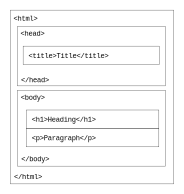
\includegraphics[keepaspectratio,width=\linewidth,height=\halfh]
    {diagrams/html-structure.pdf}

    \caption[Structure of HTML pages]{
        HTML pages are structured as a hierarchical tree of elements which enables the composition of complex structures.
        \imgcredit{Image drawn by the author of this thesis.}
    }
    \label{fig:HTMLStructure}
\end{figure}

A strong pillar of HTML's design is extensibility. There are multiple mechanisms in place to ensure applicability to a vast range of use cases. These mechanisms include:

\begin{itemize}
    \item Specifying classes of elements using the \lstinline{class} attribute. This effectively creates custom elements while still basing them on the most related, already existing elements.
    \item Using \lstinline{data-*} attributes to decorate elements with additional data that can be used by scripts. The HTML standard guarantees that these attributes are ignored by browsers.
    \item Embedding custom data using \lstinline{<script type="">} elements that can be accessed by scripts.
\end{itemize}


\section{Cascading Style Sheets (CSS)}

Cascading Style Sheets (CSS) is a style sheet language that is used to specify the presentation of a HTML document. It can either be embedded directly in HTML documents or it can be defined externally and linked into them. This characteristic of being able to externally describe the presentation of documents yields a lot of flexibility because multiple documents with different content can reuse the same presentation by linking to the same CSS file. 


It can not only be  used to describe the style of elements but also their layout. 

By not directly including presentation features in the HTML standard, a separation of concerns is achieved that improves accessibility and flexibility.

\subsection{Box Layout}
\subsection{Flexbox Layout}
\subsection{Grid Layout}

\section{JavaScript (JS)}

\section{TypeScript (TS)}

\section{Web Graphics}

\subsection{Raster Images}

\TODO{Describe raster images}

\TODO{Mention JPEG}

\TODO{Mention PNG}

\subsection{Scalable Vector Graphics (SVG)}

\TODO{Define detail in which to write about SVG}

\TODO{Describe SVG}

\TODO{Describe filters}

\TODO{Talk about issues with using CSS for styling}



SVG elements can be styled with CSS which is highly convenient as it brings all the benefits of CSS like allowing users to override parts of the styling in their own style sheets. SVG styles defined as CSS can also be animated using CSS animations and transitions. This is recommendable to manual animations using JavaScript because external configuration is inherently supported and the declarative syntax of CSS animations is powerful enough to define complex animations.

% However, SVG 1.1 \TODO{Cite spec} only supports configuration of presentation attributes via CSS and it is not possible to . Other types of attributes, like geometric attributes, can't be styled using CSS and require actual configuaration via HTML attributes. SVG 2 will support styling and animating non-presentation attributes with CSS. \TODO{Add (partial?) list of presentation attributes}\TODO{Add (partial?) list of presentation attributes}

% https://css-tricks.com/svg-properties-and-css/#svg-2
% https://stackoverflow.com/a/14258103


\subsection{Canvas}

\subsection{WebGL}

\section{Layout Engines}

\subsection{Yoga Layout}
\subsection{FaberJS}

\section{Visualization Libraries}

\subsection{Chartist}
\subsection{Highcharts}
\subsection{ECharts}
\subsection{...?}
\subsection{D3}
\TODO{Mention that D3 is successor of Protovis}

\section{Tools}
\subsection{Node}
\subsection{Rollup}
\subsection{Gulp}

         

\cleardoublepage

\chapter{Information Visualization}
\label{chap:InfoVis}

Information visualization seeks to use interactive graphics to assist
in the analysis and presentation of abstract information. Information
visualization builds on capabilities of human visual perception,
including the rapid scanning, recognition, and recall of visual
information, as well as the automatic detection of visual patterns. In
contrast to textual representations of data, the processing of
well-designed visualizations requires less cognitive effort,
because it leverages features of the human visual processing
system. One of these features is \emph{preattentive processing},
whereby certain visual attributes can be processed very quickly and
without conscious effort \parencite{PreattentiveProcessing}.
% KA give an example of a pre-attentive feature


In addition to visuals being easier to assimilate by humans, a purely
textual and statistical view of data can also lead to erroneous
assumptions. This is demonstrated in Anscombe's famous example of four
completely different datasets (variables in $x$ and $y$) having
identical summary statistics (mean and standard deviation), called
Anscombe's Quartet \parencite{AnscombesQuartet}, shown in
Table~\ref{tab:AnscombeTable}. An observer trying to understand these
datasets from their summary statistics alone might mistakenly deem
them to be identical. Their inequality only becomes obvious after
carefully examining and comparing the individual entries in the
datasets themselves.
%
However, the differences in the four datasets are immediately obvious
when plotted graphically, as can be seen in
Figure~\ref{fig:AnscombePlot}. Even though Anscombe's Quartet is
likely the most famous example demonstrating this characteristic, it
is certainly not the only example, as has been shown by
\textcite{GenDataIdenticalStatisticsDissimilarGraphics}.



\begin{table}[tp]
\centering
\tablestretch
\rowcolors{3}{tablerowcolour}{}
\begin{small}
\begin{tabular}{>{\kern-\tabcolsep}rcrrcrrcrrcrr<{\kern-\tabcolsep}}
\toprule
\hiderowcolors
  & \phantom{i} &
  \multicolumn{2}{c}{$\mathbf{v_1}$} & \phantom{a} &
  \multicolumn{2}{c}{$\mathbf{v_2}$} & \phantom{a} &
  \multicolumn{2}{c}{$\mathbf{v_3}$} & \phantom{a} &
  \multicolumn{2}{c}{$\mathbf{v_4}$} \\
\cmidrule(l{1em}r){3-4}\cmidrule(l{1em}r){6-7}\cmidrule(l{1em}r){9-10}\cmidrule(l{1em}r){12-13}
  & & $x_1$ &  $y_1$ & &  $x_2$ & $y_2$ & & $x_3$ &  $y_3$ & &  $x_4$ &  $y_4$ \\
\midrule
\showrowcolors
  & & 10.00 &   8.04 & &  10.00 &  9.14 & &  10.00 &   7.46 & &   8.00 &   6.58 \\
  & &  8.00 &   6.95 & &   8.00 &  8.14 & &   8.00 &   6.77 & &   8.00 &   5.76 \\
  & & 13.00 &   7.58 & &  13.00 &  8.74 & &  13.00 &  12.74 & &   8.00 &   7.71 \\
  & &  9.00 &   8.81 & &   9.00 &  8.77 & &   9.00 &   7.11 & &   8.00 &   8.84 \\
  & & 11.00 &   8.33 & &  11.00 &  9.26 & &  11.00 &   7.81 & &   8.00 &   8.47 \\
  & & 14.00 &   9.96 & &  14.00 &  8.10 & &  14.00 &   8.84 & &   8.00 &   7.04 \\
  & &  6.00 &   7.24 & &   6.00 &  6.13 & &   6.00 &   6.08 & &   8.00 &   5.25 \\
  & &  4.00 &   4.26 & &   4.00 &  3.10 & &   4.00 &   5.39 & &  19.00 &  12.50 \\
  & & 12.00 &  10.84 & &  12.00 &  9.13 & &  12.00 &   8.15 & &   8.00 &   5.56 \\
  & &  7.00 &   4.82 & &   7.00 &  7.26 & &   7.00 &   6.42 & &   8.00 &   7.91 \\
  & &  5.00 &   5.68 & &   5.00 &  4.74 & &   5.00 &   5.73 & &   8.00 &   6.89 \\
\hiderowcolors
\addlinespace[0.5em]
\textbf{mean} & &
  \textbf{9.00} & \textbf{7.50} & &
  \textbf{9.00} & \textbf{7.50} & &
  \textbf{9.00} & \textbf{7.50} & &
  \textbf{9.00} & \textbf{7.50} \\
\textbf{sd} & &
  \textbf{3.3166} & \textbf{2.0316} & &
  \textbf{3.3166} & \textbf{2.0317} & &
  \textbf{3.3166} & \textbf{2.0304} & &
  \textbf{3.3166} & \textbf{2.0306} \\
\bottomrule
\end{tabular}
\end{small}

\caption[Anscombe's Quartet in Tabular Form]
{
The four datasets (variables) in Anscombe's Quartet look identical if
only standard summary statistics like mean and standard deviation are
considered. The difference between the datasets is only apparent after
careful examination of the numbers.
}
\label{tab:AnscombeTable}
\end{table}



\begin{figure}[tp]
\centering
\includegraphics[keepaspectratio,width=\linewidth,height=\halfh]
{diagrams/anscombe.pdf}
\caption[Anscombe's Quartet]{
When plotted graphically, it is immediately apparent that
the four datasets in Anscombe's Quartet are very different.
\imgcredit{Image extracted from \textcite{IVISCourseNotes}.
Used with kind permission by Keith Andrews.}
}
\label{fig:AnscombePlot}
\end{figure}







This thesis adheres to the characterization of the field of
visualization as having three main subfields, as defined by
\textcite{IVISCourseNotes}:
\begin{enumerate}
\item \liintro{Information Visualization (InfoVis)}: Deals with
  abstract data, which has no inherent geometry or visual form and for
  which a suitable type of visualization has to be chosen.

\item \liintro{Geographic Visualization (GeoVis)}: Deals with
  map-based data which has inherent 2d or 3d spatial geometry.

\item \liintro{Scientific Visualization (SciVis)}: Deals with
  real-world objects having inherent 2d or 3d geometry, which
  is used as the basis for visualization.
\end{enumerate}
The often-used term \enquote{data visualization} (\emph{DataVis}) is
defined as the combination (union) of information visualization and
geographic visualization.


Visualizations presented in an interactive medium do not merely
consist of visual representations. It is equally important to provide
means for interacting with these representations to analyze more
complex datasets. Without interactions, a visualization is just a
static image and has only very limited use when dealing with large and
multidimensional datasets. Even though the majority of attention in
the field of information visualization has been directed towards the
presentational aspect of visualizations, research has also been done
on their interactive aspects. Numerous taxonomies have been formulated
with the goal of defining the design space of interactions to support
analytic reasoning, but they vary greatly depending on the concepts
they are focusing on. Some taxonomies have been defined on the concept
of low-level interaction techniques
\parencite{TheEyesHaveIt,GrammarOfGraphics}, providing a very
system-centric view on interaction. Other taxonomies focus on user
tasks \parencite{LowLevelComponentsOfAnalyticActivity}, which are not
necessarily strongly related to interacting with visualizations.
\textcite{RoleOfInteractionInInformationVisualization} aims to provide
a view in between the purely system-centric and purely user-centric
extremes by defining a taxonomy based on what a user wants to achieve,
also known as \emph{user intent}. The categories of this taxonomy are
shown in Table~\ref{tab:UserIntentCategories}. They provide a good
framework for the discussion of interactivity in the context of
information visualization.


\begin{table}[tp]
\tablestretch
\rowcolors{2}{}{tablerowcolour}
\centering
\begin{small}
\begin{tabularx}{\linewidth}{>{\kern-\tabcolsep}lL{0.35\linewidth}X<{\kern-\tabcolsep}}
\toprule
Category & Description & Examples \\
\midrule
Select &
  Mark something as interesting. &
  Highlighted selections, placemarks, assigning classes. \\
Explore &
  Show me something else. &
  Different subset of data, panning, direct-walk. \\
Reconfigure &
  Show me a different arrangement. &
  Sorting, rearranging columns, plotting different dimensions, using an alternative projection. \\
Encode &
  Show me a different representation. &
  Changing visual encoding (color, size, shape), or even chart type. \\
Abstract / Elaborate &
  Show me more or less detail. &
  Details-on-demand, drill-down and roll-up, tooltips, zooming in and out. \\
Filter &
  Show me something conditionally. &
  Dynamic queries, range sliders, toggle buttons, query by example. \\
Connect &
  Show me related items. &
  Brushing across views, highlighting connected items on mouseover. \\
\bottomrule
\end{tabularx}
\end{small}
\caption[Categories of Interaction Based on User Intent]{
Categories of interaction with visualizations based on what
a user wants to achieve (user intent).
\imgcredit{From \textcite{RoleOfInteractionInInformationVisualization}}
}
\label{tab:UserIntentCategories}
\end{table}






\section{History of Information Visualization}

The history of information visualization goes back a long time. One of
its earliest examples dates back to the \nth{10} Century, when an
unknown astronomer created the chart about the movement of prominent
planets \parencite{CommentariiInSomniumScipionis} shown in
Figure~\ref{fig:PlanetaryMovements}.
% KA: 1175 is the 12th Century not the 10th
Other noteworthy early visualizations include the first occurrence of
the principle which \textcite{VisualDisplayOfQuantitativeInformation}
later called \enquote{small multiples} in the 1626 chart by
\textcite{RosaUrsina} demonstrating sunspot changes shown in
Figure~\ref{fig:SunspotChanges}, and the 1644 chart displaying
longitudinal distance determinations between Toledo and Rome by
Michael Florent van Langren shown in
Figure~\ref{fig:RomeToledoLongitude}.


\begin{figure}[tp]
\centering
\includegraphics[keepaspectratio,width=\linewidth,height=\thirdh]
{images/planetary-movements.png}
\caption[Chart of Planetary Movements from the \nth{10} Century]{%
A line chart created by an unknown astronomer in the \nth{10} Century,
depicting the movements of seven prominent planets.
\imgcredit{Image extracted from \textcite{BriefHistoryOfDataVis}.
Original appearance in \textcite{CommentariiInSomniumScipionis}.}
}
\label{fig:PlanetaryMovements}
\end{figure}
% KA Original appearance in Macrobius [1175] ??
% Funkhouser 1936 says 10th or 11th Century



\begin{figure}[tp]
\centering
\includegraphics[keepaspectratio,width=\linewidth,height=\thirdh]
{images/sunspot-changes.png}
\caption[Chart of Changes in Sunspots from 1626]{%
The observed changes in sunspots based on recordings
of two months of data from 1611. It is the first occurrence of the
principle later called \enquote{small multiples} by
\textcite{VisualDisplayOfQuantitativeInformation}.
\imgcredit{Image extracted from \textcite{BriefHistoryOfDataVis}.
Original appearance in \textcite{RosaUrsina}.}
}
\label{fig:SunspotChanges}
\end{figure}

% https://cudl.lib.cam.ac.uk/view/PR-QQ-AST-00002-00158-B-00003/1

% Tufte, Edward R. and Peter R. Graves-Morris [1983].
% The Visual Display of Quantitative Information.
% Graphics Press, 1983. ISBN 1930824130 (cited on pages 19–20).
% KA: who is Graves-Morris ?



\begin{figure}[tp]
\centering
\includegraphics[keepaspectratio,width=\linewidth,height=\thirdh]
{images/rome-toledo-longitude.png}
\caption[Chart of Longitudinal Distance Determinations Between Toledo and Rome From 1644]{%
A comparison of the twelve known estimates in longitudinal
distance between Rome and Toledo by various astronomers. The correct
distance is marked by the arrow beneath. It is considered to be the
first visual representation of statistical data.
\imgcredit{Image extracted from \textcite{BriefHistoryOfDataVis}.
Original appearance in \textcite{VisualExplanations}.}
}
\label{fig:RomeToledoLongitude}
\end{figure}

% KA  how can it be the "first visual representation of statistical data"  ?

% Tufte, Visual Explanations, 1997, page 15





William Playfair (1759--1823) is considered by many to be one of the
forefathers of modern information visualization. His published works
contain the first occurrences of many graphical forms still widely
used today. In one of his earlier works
\parencite{CommercialAndPoliticalAtlas}, he introduced the concepts of
line charts (Figure~\ref{fig:PlayfairLineChart}), bar charts
(Figure~\ref{fig:PlayfairBarChart}), and area charts
(Figure~\ref{fig:PlayfairAreaChart}) to communicate economic factors
of England during the eighteenth century. In a related later work
\parencite{StatisticalBreviary}, he used the first ever published pie
and circle charts to show and compare the resources of states and
kingdoms in Europe. The charts he created are very similar to modern
ones, containing familiar concepts such as labeled axes, grids,
titles, and color-coding.



\begin{figure}[tp]
\centering
\includegraphics[keepaspectratio,width=\linewidth,height=\thirdh]
{images/playfair-line-chart.png}
\caption[Line Chart by William Playfair from 1786]{%
Line chart of the expenditure of the British Navy during the \nth{18}
Century. It was published in 1786 and is considered to be one of the
first occurrences of a line chart containing components found in
modern visualizations.
\imgcredit{Image extracted from Schoenberg Center for
Electronic Text and Image (SCETI).
Used under the terms of Creative Commons CC BY 2.5.}
}
\label{fig:PlayfairLineChart}
\end{figure}



\begin{figure}[tp]
\centering
\includegraphics[keepaspectratio,width=\linewidth,height=\thirdh]
{images/playfair-bar-chart.png}
\caption[Bar Chart by William Playfair from 1786]{%
Bar chart of England's exports and imports to and from Scotland in
1781. Published in 1786, it is considered to be one of the
first occurrences of a bar chart containing most components found in
modern visualizations.
\imgcredit{Image extracted from Schoenberg Center
for Electronic Text and Image (SCETI).
Used under the terms of Creative Commons CC BY 2.5.}
}
\label{fig:PlayfairBarChart}
\end{figure}



\begin{figure}[tp]
\centering
\includegraphics[keepaspectratio,width=\linewidth,height=\thirdh]
{images/playfair-area-chart.png}
\caption[Area Chart by William Playfair from 1786]{%
Area chart of annual revenues of England and France between
1550 and 1800. Published in 1786, it is considered to be one of
the first occurrences of an area chart
containing most components found in modern visualizations.
\imgcredit{Image extracted from Schoenberg Center
for Electronic Text and Image (SCETI).
Used under the terms of Creative Commons CC BY 2.5.}
}
\label{fig:PlayfairAreaChart}
\end{figure}




%% The dot map created by \textcite{ModeOfCommunicationOfCholera} in 1855
%% to trace cholera outbreaks in London (Figure~\ref{fig:CholeraDotMap})
%% is undoubtedly one of the most famous and influential visualizations
%% in history.  Even though it is not directly an information
%% visualization but rather a geographic one, it has been included here
%% because of its historic relevance.  This iconic dot map was used to
%% identify a cluster of cholera-related deaths near a contaminated water
%% pump on Broad Street, leading to the recognition of cholera as a
%% waterborne disease.
%% 
%% 
%% \begin{figure}[tp]
%% \centering
%% \includegraphics[keepaspectratio,width=\linewidth,height=\fullh / 3]{images/cholera-dot-map.png}
%% \caption[Dot Map Plotting Cholera Deaths in London From 1855]{%
%% This iconic chart was created by Dr. John Snow in 1855 to identify a
%% clustering of cholera-related deaths near Broad Street in London.  It
%% was used to identify a contaminated water pump and to illustrate the
%% waterborne nature of the disease.  Since the data is map-based, this
%% chart is an example of a geographic visualization rather than an
%% information visualization.
%% \imgcredit{Image extracted from \textcite{IVISCourseNotes}.
%% Original appearance in \textcite{ModeOfCommunicationOfCholera}.}
%% }
%% \label{fig:CholeraDotMap}
%% \end{figure}






It would be amiss not to mention Florence Nightingale (1820--1910)
\parencite{FlorenceNightingale} when talking about the history of
information visualization. She was a British statistician, social
reformer, and the founder of modern nursing and might be the first
person who used visualizations to persuade others of a need for
change. During her service as a superintendent of nurses in the
Crimean War, she realized that a large number of deaths in hospitals
resulted from preventable diseases which originated in poor sanitary
conditions. One of her contributions to the field of information
visualization was the creation of a new type of diagram, called a rose
diagram or polar-area chart, shown in
Figure~\ref{fig:NightingalePolarAreaChart}. She used these charts to
communicate data she collected on the mortality of soldiers during the
war and to grab the attention of politicians and the public.

\begin{figure}[tp]
\centering
\includegraphics[keepaspectratio,width=\linewidth,height=\thirdh]
{images/nightingale.png}
\caption[Polar-Area Chart by Florence Nightingale from 1859]{%
One of the polar-area charts created by Florence Nightingale in 1859
to convince people of a need for more sanitary conditions in
hospitals. It visualizes the causes of mortality for soldiers during
the Crimean War and demonstrates that a large percentage of patients
died from preventable diseases linked to unsanitary environments.
\imgcredit{Image extracted from Harvard Library.
Used under the terms of Creative Commons Attribution 4.0.}
}
\label{fig:NightingalePolarAreaChart}
\end{figure}




Modern visualizations benefit from the interactive nature of the
devices used to consume them. They can be more complex than static
visualizations, because various interaction techniques enable users to
navigate large amounts of data and make sense of it. High-D by
Macrofocus \parencite{HighD} is a representative example of a modern
interactive visual analytics tool, and is shown in
Figure~\ref{fig:HighD}.

\begin{figure}[tp]
\centering
\includegraphics[keepaspectratio,width=\linewidth,height=\thirdh]
{images/high-d.png}
\caption[High-D]{
High-D by Macrofocus is a visual analytics tool
specialized in analyzing multidimensional data.
\imgcredit{Screenshot of High-D \parencite{HighD} taken by the author of this work.}
}
\label{fig:HighD}
\end{figure}




It is out of the scope of this work to provide a full account of the
long and eventful history of information visualization. This section
only provides a brief and very selective view of the topic.  More
comprehensive works for further reading include
\textcite{BriefHistoryOfDataVis},
\textcite{HistoryOfDataVisAndGraphicCommunication}, and
\textcite{HistoryOfInformationGraphics}.









\section{Information Visualization Libraries for the Web}

There are many web-based libraries which simplify the rendering of
interactive visualizations.  The approaches used to create and update
visualization can be vastly different between libraries.  D3 is a
low-level library which enables data-driven transformations of
documents, Vega and Vega-Lite provide a declarative grammar which
enables the expression of visual and interactive characteristics of
visualizations, and template-based visualization libraries provide a
template-based interface which can easily be configured.  These
libraries and some of their characteristics will be summarized in the
following sections.



\subsection{Data-Driven Documents (D3)}

D3 \parencite{D3} is a free and open-source document manipulation
library built in JavaScript.  It is maintained by an active GitHub
community and its core maintainer Mike Bostock who is also the creator
of Observable \parencite{Observable} and the deprecated Protovis
visualization library \parencite{Protovis}.

D3 enables data-driven document transformations to allow developers to
describe documents as functions of data.  As an example, developers
can define transformations which receive a dataset and transform it
into a basic HTML table or into a more sophisticated visualization as
an SVG chart.  This focus on explicitly defining transformations is
better suited for dynamic visualizations because developers have
complete control over the creation, modification and removal of
elements.  It also sets D3 apart from other visualization libraries
where developers usually define the desired state of a representation
using a declarative domain specific language.

In contrast to other visualization libraries, D3 contains no
proprietary visual primitives and relies on well established web
standards like HTML, SVG and CSS to provide visual representations.
This yields great flexibility because developers work directly with
web standards that are implemented by their browsers and do not need
to wait for D3 to implement support for new features as standards
evolve.  If developers chose to switch to a different library, the
knowledge of web standards they gained during their work with D3 might
be applicable in their future work.  The reliance on web standards
also makes it possible to use debugging tools which are already
natively implemented in browsers.

Other important aspects of D3's design include immediate evaluation,
the principle of parsimony, and support for method chaining.
Immediately evaluating functions means that operations, such as
modifying attributes, are applied instantaneously at the time of
calling the respective functions.  This achieves a reduction in
internal complexity by handing control flow decisions over to invoking
code.  It also avoids common errors related to missing state changes
when state is being modified multiple times between rendering in
libraries that build on delayed evaluation.  The principle of
parsimony, also referred to as Occam's razor, is a problem-solving
principle which stems from the field of philosophy
\parencite{PrincipleOfParsimony}.  It is frequently paraphrased as
"entities should not be multiplied beyond necessity" and when applied
to API design it means that superfluous functions in an API should be
avoided.  As an example, the background color of a circle element can
already be set with the generic \lstinline{Selection.attr} method to
set the \attrname{background-color} attribute of all elements in a
Selection.  Adding an additional \lstinline{backgroundColor} method
would violate the principle of parsimony because it would introduce a
special method to achieve something that was already achievable.
Method chaining is a popular syntax which allows functions to be
chained after one another.  The use of method chaining avoids having
to store intermediate method results into variables which would
otherwise not be needed.  It is implemented in D3 by returning the
\lstinline{Selection} on which a modifying method is called as a
result of that method.  Methods that insert new elements into the DOM,
such as \lstinline{Selection.append} and \lstinline{Selection.insert},
return a Selection of the newly added elements to enable the creation
of nested structures.  This method chaining syntax is further aided by
the \lstinline{Selection.call} method, which invokes a callback
receiving the current Selection as a parameter and returns the
original Selection to further chain methods on it after the callback
has been executed.  The \lstinline{Selection.call} method enables the
creation of complex method chaining structures and is widely used by
developers.  A simple example of method chaining in D3 and the
application of the \lstinline{Selection.call} method can be seen in
Listing~\ref{list:D3MethodChaining}.


\begin{samepage}
\lstinputlisting[%
  float=tp,
  aboveskip=\floatsep,
  belowskip=\floatsep,
  xleftmargin=0cm,              % no extra margins for floats
  xrightmargin=0cm,             % no extra margins for floats
  %
  language=JavaScript,
  basicstyle=\footnotesize\ttfamily,
  frame=shadowbox,
  numbers=left,
  label=list:D3MethodChaining,
  caption={[D3 Method Chaining] 
    A simple example of method chaining in D3 which creates an \elname{h1} and \elname{p} element inside a \elname{body}.
  },
]{listings/d3-method-chaining.js}
\end{samepage}


Selections have already been mentioned in the previous paragraphs.
They are the atomic building blocks of D3 and are used to access
almost any functionality.  Selections are created using the
\lstinline{d3.select} or \lstinline{d3.selectAll} methods.  These
methods are built on the DOM Selectors API, namely the
\lstinline{querySelector} and \lstinline{querySelectorAll} methods,
which allow the selection of elements via CSS selectors (see
Section~\ref{sec:CSS}).  The \lstinline{d3.select} and
\lstinline{d3.selectAll} methods respectively create a Selection
containing either a single element matching the provided selector, or
multiple elements matching it.  A Selection acts as a wrapper
container around selected elements to perform frequently performed DOM
operations on them.  Among others, the element operations provided by
a Selection include the setting and getting of: Attributes using the
\lstinline{Selection.attr} method, styles using the
\lstinline{Selection.style} method, properties using the
\lstinline{Selection.property} method, text or HTML content using the
\lstinline{Selection.text} or \lstinline{Selection.html} methods, and
event listeners using the \lstinline{Selection.on} method.  Selections
also provide wrapper methods to insert additional elements using the
\lstinline{Selection.append} or \lstinline{Selection.insert} methods
as well as to remove them using the \lstinline{Selection.remove}
method.  Accessing the DOM via this wrapper is less tedious than
accessing it directly because the native DOM API is very verbose, and
also because the method chaining API provided by D3 does not require
the storage of unnecessary intermediate variables.

An additional feature that D3 adds is the ability to bind data to
elements using the \lstinline{Selection.data} and
\lstinline{Selection.datum} methods.  The \lstinline{Selection.datum}
method binds a single provided data record to all elements in the
Selection, whereas the \lstinline{Selection.data} method receives an
array of data records and binds each individual data record to exactly
one element.  The \lstinline{Selection.data} method performs a join
operation between data and elements to ensure that exactly one element
per data record exists.  This data join results in three separate
Selections: the enter Selection, containing the elements which were
newly created, the update Selection, containing the elements which
merely receive new data, and the exit Selection, containing the
elements which are being removed.  Each of these Selections can be
individually transformed using the \lstinline{Selection.join} method,
which can receive three callbacks each being respectively invoked with
the enter, update and exit Selections of the data join.  This ability
of individually controlling updates of entering, updating and exiting
elements is being referred to as the general update pattern in D3 and
a simple demonstration of how it is used can be seen in
Figure~\ref{list:D3GeneralUpdatePattern}.  All the previously
mentioned DOM wrapper methods can receive either constant values or
dynamic ones, which are defined as functions.  These functions receive
the bound element data, the element's index in the group of nodes
represented by the Selection, and the group of nodes themselves as
input and calculate a dynamic value based on these parameters, which
is then forwarded to the corresponding DOM methods.


\begin{samepage}
\lstinputlisting[%
  float=tp,
  aboveskip=\floatsep,
  belowskip=\floatsep,
  xleftmargin=0cm,              % no extra margins for floats
  xrightmargin=0cm,             % no extra margins for floats
  %
  basicstyle=\footnotesize\ttfamily,
  frame=shadowbox,
  numbers=left,
  label=list:D3GeneralUpdatePattern,
  caption={[D3 General Update Pattern] 
    A demonstration of D3's general update pattern and how it can be used to specify different transformations for entering, updating and exiting elements.
    This code is merely meant as an example of how the join selections can be transformed.
    The full utility of this pattern will only be appearant in more complex scenarios that involve transitions.
  },
]{listings/d3-join.js}
\end{samepage}



D3 also offers a convenient and optional API to perform
JavaScript-based animations via Transitions, which wrap a Selection
and allow the animation of various element characteristics.
Transitions are created using the \lstinline{Selection.transition}
method which creates a Transition wrapping the Selection on which it
has been called.  The duration of a Transition is defined using the
\lstinline{Transition.duration} method and its easing can be
configured using the \lstinline{Transition.ease} method.  There is
also the possibility of interrupting and chaining transitions, but
explaining these things would be to go into too many details.
Transitions provide an almost identical API to Selections.  The major
change is that the wrapping methods interpolate towards their target
values using the set easing function over the set duration instead of
setting the target value directly.  Using D3 Transitions is completely
optional and users can also choose to instead use other animation
technologies, like CSS transitions and animations.

At the core, D3 is simply a low-level library to perform data-driven
document transformations.  Even though this generic core technology is
applicable to a wide range of use cases, D3 has been created with a
focus on creating visualizations.  There are many additional modules
which simplify performing the higher-level tasks necessary for the
rendering of visualizations.  All modules follow the same patterns
inherent to D3, like method chaining and configurable functions.
Therefore, despite these higher-level functionalities being split on
multiple modules, a consistent experience is provided to developers.
Listing all available modules here would be out of the scope of this
work, but some noteworthy and characteristic ones include:
\modname{d3-shape} to create visual primitives like lines and areas,
\modname{d3-scale} to encode abstract data dimensions,
\modname{d3-axis} to render scales as human-readable axes, and many
more such as \modname{d3-array}, \modname{d3-layout} and
\modname{d3-zoom}.



\subsection{Vega and Vega-Lite}

Vega \parencite{Vega} is a library which consists of a grammar to
describe interactive graphics and a parser which translates
specifications written in this grammar into static images or web-based
views built on SVG documents or the Canvas Web API.  An interactive
visualization in Vega is fully described by a specification written in
Vega's grammar.  This grammar is essentially a domain specific
language designed for the declarative denotation of interactive
graphics.  Its syntax is based on the easy-to-read JavaScript Object
Notation (JSON), which is among the most frequently used textual
serialization formats.  Vega builds on previous research in the field
of declarative visualization design \parencite{GrammarOfGraphics}.
Compared to previous works, it contains powerful capabilities to
declaratively describe interactions \parencite{ReactiveVega} in
addition to describing visual appearances.

The visual aspects of a visualization are described in a grammar
similar to the one defined by \textcite{GrammarOfGraphics}.  At its
top level, a Vega specification contains properties to configure
sizing and padding of the container of a visualization.  Every
specification will also contain a data section which either defines
data or specifies where to load it from.  The Vega grammar also
supports various forms of data transformation which can successively
be applied to a dataset to perform various transformations like
filtering, deriving additional fields or deriving additional datasets.
In a majority of cases, the defined data will consist of abstract
information that requires being mapped to visual properties.  This
mapping is configured and performed using scales.  Vega already
contains a variety of scales to help with mapping abstract values to
visual properties.  They can broadly be categorized into quantitative
scales which map quantitative inputs to quantitative outputs, discrete
scales which map discrete inputs to discrete outputs, and discretizing
scales which map quantitative inputs to discrete outputs.  For
spatially encoded dimensions, these scales can be visualized as axes,
whereas non-spatial encodings such as encodings as colors, sizes or
shapes can be visualized as legends.  At the core of every
visualization lies the encoding of data as visual primitives, which is
achieved in Vega via marks.  Marks use scales to encode data fields as
properties of their shapes.  Based on the general update pattern of
the underlying D3 library, the encoding of marks can be separately
controlled for newly created (entering) marks, existing and not
exiting (updating) marks, and to-be-removed (exiting) marks.  In
addition to these basic visualization components, the Vega grammar
contains further capabilities to describe interactions (via signals,
triggers and event streams), cartographic projections, sequential or
layered views (via mark groups), layouts and color schemes.  To
demonstrate how the various aspects of a Vega specification are
defined, an example which represents a static bar chart can be seen in
Listing~\ref{list:VegaStaticBarChart}.


\begin{samepage}
\lstinputlisting[%
  float=tp,
  aboveskip=\floatsep,
  belowskip=\floatsep,
  xleftmargin=0cm,              % no extra margins for floats
  xrightmargin=0cm,             % no extra margins for floats
  %
  basicstyle=\footnotesize\ttfamily,
  frame=shadowbox,
  numbers=left,
  label=list:VegaStaticBarChart,
  caption={[Static Bar Chart in Vega] 
    The Vega specification of a static bar chart.
    Demonstrates the principle of data, scales, axes and marks.
  },
]{listings/vega-static-bar-chart.json}
\end{samepage}


In template-based visualization libraries, interactions are typically
defined by configuring premade interaction templates, which is easy
but limiting, or by manually modifying the visualization in various
callbacks, which is flexible but tedious and not serializable.  The
ability to describe custom interactions using a serializable,
data-driven grammar is what sets Vega apart from other declarative
visualization libraries.  This approach offers a comparable
flexibility to callback-driven interactions while still remaining
fully serializable and declarative.  The grammar to define
interactions is based on the syntax of event-driven functional
reactive programming \parencite{EventDrivenFRP}, a high-level grammar
which resembles mathematical equations to describe reactive systems.
In Vega, the primitives to express interactions are called signals.
Signals can be seen as dynamic variables which change their values
based on input events or other signals.  These signals and the way
their values change are declaratively defined, and they can be used as
dynamic variables throughout most places in a Vega specification to
change various characteristics of a visualization dynamically.  An
example of how the previously demonstrated static bar chart
specification can be extended with signals to display a tooltip when
hovering over bars can be seen in Listing~\ref{list:VegaBarChart}.


\begin{samepage}
\lstinputlisting[%
  float=tp,
  aboveskip=\floatsep,
  belowskip=\floatsep,
  xleftmargin=0cm,              % no extra margins for floats
  xrightmargin=0cm,             % no extra margins for floats
  %
  basicstyle=\footnotesize\ttfamily,
  frame=shadowbox,
  numbers=left,
  label=list:VegaBarChart,
  caption={[Bar Chart with Tooltip in Vega] 
    The necessary additions to the static bar chart specification in Listing~\ref{list:VegaStaticBarChart} to display a tooltip when hovering over bars.
    It demonstrates the basic functionality of signals in Vega.
    When the mouse hovers over a rect mark, the tooltip signal will receive the value of the rect's bound data record.
    The tooltip signal will be reset to an empty object when the mouse leaves the rect mark.
    It is then used in the newly added text mark section of the specification to define the position, text and visibility of it whenever an update occurs.
  },
]{listings/vega-bar-chart.json}
\end{samepage}



Visualizations created with Vega closely follow their specifications
and minimal assumptions are being made in the compilation process.
This results in very verbose specifications because all configurations
for all parts of the visualization need to be explicitly defined in
them.  It also means that specification authors have full control over
the resulting graphics, making Vega a good base on which to build
further libraries and tools.  Many tools
\parencite{Voyager,Lyra,CompassQL} have already been built on top of
Vega.  The tool worth mentioning most is Vega-Lite
\parencite{VegaLite}.  Vega-Lite is described as a "high-level grammar
of interactive graphics", which summarizes its difference to Vega
fairly well.  Vega-Lite is a higher-level grammar than Vega, which
allows authors to write specifications for common visualizations in a
much more concise form.  Specifications written in Vega-Lite are
compiled into Vega specifications.  During compilation, the compiler
automatically derives default configurations for axes, legends and
scales from a set of carefully designed rules.  This makes Vega-Lite
more convenient to use for quick authoring of visualizations because
many details which need to be explicitly stated in a Vega
specification can be omitted.  In those cases where the derived
default configurations are not suitable, Vega-Lite also offers the
possibility to override them.  Since Vega-Lite specifications are
simply being compiled into Vega ones, it is a sensible choice to use
Vega-Lite as a primary tool to describe visualizations, and switch to
Vega for more exotic cases which are not easily achievable in
Vega-Lite.  To properly compare the difference between Vega and
Vega-Lite specifications, a Vega-Lite version of the Vega bar chart
specification seen in Listing~\ref{list:VegaStaticBarChart} combined
with Listing~\ref{list:VegaBarChart} can be seen in
Listing~\ref{list:VegaLiteBarChart}.


\begin{samepage}
\lstinputlisting[%
  float=tp,
  aboveskip=\floatsep,
  belowskip=\floatsep,
  xleftmargin=0cm,              % no extra margins for floats
  xrightmargin=0cm,             % no extra margins for floats
  %
  basicstyle=\footnotesize\ttfamily,
  frame=shadowbox,
  numbers=left,
  label=list:VegaLiteBarChart,
  caption={[Bar Chart with Tooltip in Vega-Lite] 
    This is a Vega-Lite specification of the Vega bar chart specification seen in Listing~\ref{list:VegaStaticBarChart} combined with Listing~\ref{list:VegaBarChart}.
  },
]{listings/vega-lite-bar-chart.json}
\end{samepage}




\subsection{Template-Based Visualization Libraries}

Template-based visualization libraries work by providing templates for
possible types of visualizations and allowing users to customize them.
These types of visualization libraries are easier to use than D3 or
Vega because they offer a concise form of configuration which does not
require users to have detailed knowledge over the underlying rendering
technology or complex, non-standardized domain specific languages.
Even though these types of libraries are usually flexible enough to
create a huge range of visualizations, at one point users may run into
limitations.  Some of these limitations can not be worked around and
require the writing of custom source code which requires a deep
understanding of the underlying library.  This effectively eliminates
the ease-of-use benefit of these types of libraries for users that run
into these limitations.

For this thesis, a total of 20 template-based JavaScript visualization
libraries have been collected and compared by different factors such
as their rendering technology, usage popularity, open-source
popularity, license, and recent development activity.  In terms of
rendering technology, most libraries render visualizations as either
SVG documents or canvas elements, though some implement a hybrid
renderer which can be configured to render as either one of them.
Usage popularity has been measured by the cumulative package downloads
from the npm package manager over the last twelve months.  This has
been deemed one of the most relevant metrics for the comparison
because it reflects actual user behavior and gives an indication on
how widespread a library is used in practice.  The 20 libraries found
in the initial collection phase were filtered by their usage
popularity and recent development activity to remove those which were
not sufficiently used or maintained anymore.  This filtering step
yielded the following ten libraries: (1) ChartJS \parencite{ChartJS},
(2) Highcharts \parencite{Highcharts}, (3) ECharts
\parencite{ECharts}, (4) ApexCharts \parencite{ApexCharts}, (5)
PlotlyJS \parencite{PlotlyJS}, (6) C3JS \parencite{C3JS}, (7) Chartist
\parencite{Chartist}, (8) amCharts \parencite{amCharts}, (9)
billboardJS \parencite{billboardJS}, and (10) D3FC \parencite{D3FC}.
These libraries have been selected for deeper evaluation because they
are heavily used and, for the most part, still actively maintained.
The focus of this more detailed analysis is on summarizing these
libraries based on high-level features and responsive capabilities.

Eight of those ten libraries are completely free to use without
restrictions, amCharts has a free license for users who are
comfortable with an attribution logo on their visualizations, and
Highcharts offers a free license option for non-profit, educational
and personal applications.  Nine libraries implement an SVG-based
renderer, two of which (ECharts, D3FC) offer alternative rendering to
canvas elements for high-performance scenarios, and only ChartJS
purely targets canvas-based rendering.  Eight libraries are very
actively maintained with most of them showing development activity
within the last month.  Only C3JS and Chartist do not seem to be
actively maintained anymore, but they nonetheless have been included
in the deeper evaluation because of their historic and thematic
relevance and because they are still widely used.

Template-based visualization libraries have a strong inclination
towards designing their APIs according to principles of declarative
programming.  APIs following these principles allow users to describe
a desired state they want the underlying system to be in.  This is in
strong contrast to the typical imperative way of designing APIs in
which users are instead given a set of tools to query and modify a
system's state.  The difference can be summarized in simple terms as:
Using declarative APIs, users specify what state shall be achieved,
whereas when using imperative APIs, users specify how a certain state
is achieved.  Declarative APIs are typically built on top of
lower-level imperative APIs and can therefore be seen as a higher
level of abstraction over them.  They are popular among developers
because they are expressive, easy to use and effectively encapsulate
complexity which would otherwise have to be handled by users.  An
often overlooked disadvantage of declarative APIs is that they
frequently only provide high-level access to a system and that more
specific use cases might not be achievable if they can not be
expressed in the domain specific language defined by the API.  In many
cases it makes sense to provide additional imperative APIs for users
which require a lower level of access to the system to implement
functionality not achievable via the declarative parts of the
interface.

All evaluated libraries, except D3FC, expose declarative interfaces in
the form of nested configuration objects which are used to specify the
characteristics of individual visualizations.  Apart from Chartist,
all those libraries feature generic high-level creation functions.
These functions create charts from declarative configuration objects,
which allow the specification of different forms of visualization for
different data dimensions.  This type of interface is demonstrated by
the Highcharts code seen in Listing~\ref{list:Highcharts}.  Generic
chart creation functions seem to be correlated with the ability of
dynamically changing the type of visualization.  In Chartist, for
instance, which provides separate chart creation functions for each
type of chart, it is not possible to alter the type of chart after it
has been created.  Another limitation which may originate in this
interface partitioning via chart types is that mixed charts which
combine multiple forms of visualization in one composite visualization
can not be expressed.  The only library in the deeper evaluation which
does not provide a high-level declarative configuration API is D3FC.
The design philosophy of D3FC is based on the idea of "unboxing" D3.
Even though many visualization libraries are implemented on top of D3,
it is usually hidden behind public APIs which are easier to work with
but do not provide the full flexibility of D3.  D3FC exposes a
component-based interface which closely follows design patterns
frequently encountered when working with D3.  These components form
higher-level building blocks on which advanced visualizations can be
built.  They are also highly configurable and in those cases where the
options for configuration are not sufficient, a decorator pattern is
used to allow users to hook into the underlying D3 functionality and
inject custom code into the various stages of the general update
pattern at the core of D3.  Code which demonstrates the usage of D3FC
can be seen in Listing~\ref{list:D3FC}.  The only evaluated library
which exposes a hybrid API with the possibility of configuring
visualizations using both declarative configuration objects and
manually composing higher-level visualizations from lower-level
components, such as axes and series, is amCharts.  Its component-based
interface is still rather declarative, with most options being
configurable by modifying certain properties on the components.
However, modifying only the properties which require changing instead
of processing a full configuration object and figuring out the
necessary changes from it is less costly in terms of performance.  In
addition to these performance benefits, the components provide
additional functions to perform operations which would not be
available using a purely declarative API.



\begin{samepage}
\lstinputlisting[%
  float=tp,
  aboveskip=\floatsep,
  belowskip=\floatsep,
  xleftmargin=0cm,              % no extra margins for floats
  xrightmargin=0cm,             % no extra margins for floats
  %
  basicstyle=\footnotesize\ttfamily,
  frame=shadowbox,
  numbers=left,
  label=list:Highcharts,
  caption={[Bar Chart in Highcharts] 
    This example demonstrates how a basic column (vertical bar) chart is defined using the generic chart creation API provided by Highcharts.
  },
]{listings/highcharts.js}
\end{samepage}



\begin{samepage}
\lstinputlisting[%
  float=tp,
  aboveskip=\floatsep,
  belowskip=\floatsep,
  xleftmargin=0cm,              % no extra margins for floats
  xrightmargin=0cm,             % no extra margins for floats
  %
  basicstyle=\footnotesize\ttfamily,
  frame=shadowbox,
  numbers=left,
  label=list:D3FC,
  caption={[Bar Chart in D3FC] 
    This example demonstrates how a basic bar chart is defined using the component-based API provided by D3FC.
  },
]{listings/d3fc.js}
\end{samepage}



When comparing the evaluated libraries by their responsive
configurability, most libraries offer similar capabilities albeit in
slightly different ways.  Six libraries (Highcharts, C3JS, Chartist,
amCharts, billboardJS, D3FC) support the styling of elements in their
created visualizations with CSS, which requires rendering as SVG
documents because only document-based visualizations can be affected
by CSS.  The styling of visualizations with CSS is powerful because it
leads to a separation of concerns and designers can make use of
CSS-inherent mechanisms to configure responsive styles.
Unfortunately, CSS-based styling is only of limited applicability
because not all CSS properties affect SVG elements, which has already
been described in Section~\ref{sec:SVG}.  To responsively configure
other visualization characteristics, such as their type, data, and
layout, designers have to resort to configuration mechanisms offered
by the libraries.  Four libraries (Highcharts, ApexCharts, Chartist,
amCharts) provide the possibility to specify rule-based responsive
configurations as part of their declarative interfaces, demonstrated
in the Highcharts example in Listing~\ref{list:HighchartsResponsive}.
These declarative rules consist of a condition part which specifies
when to apply the rule, and a configuration part which specifies the
configuration options which should be set when applying the rule.
Even though this is a convenient form of responsive configuration, if
the desired conditions can not be expressed via the provided
declarative properties, designers have to fall back to more generic
mechanisms which are also applicable to other libraries.  The
mechanisms for responsive configuration in the other libraries are
more generic because they do not offer these configurations as part of
their declarative interfaces.  This means that developers need to
trigger responsive configurations themselves by manually reconfiguring
visualizations via their APIs in custom resize or media query event
listeners.  Nearly all libraries provide means to dynamically resize
visualizations and update their data, type and options.  The
exceptions from this are C3JS, which only supports dynamic changes of
some options, and Chartist, which does not support changing of a
visualization's type.



\begin{samepage}
\lstinputlisting[%
  float=tp,
  aboveskip=\floatsep,
  belowskip=\floatsep,
  xleftmargin=0cm,              % no extra margins for floats
  xrightmargin=0cm,             % no extra margins for floats
  %
  basicstyle=\footnotesize\ttfamily,
  frame=shadowbox,
  numbers=left,
  label=list:HighchartsResponsive,
  caption={[Responsive Rules in Highcharts] 
    This example demonstrates how responsive rules can be declared to configure various aspects of a visualization in relation to the size of the viewport.
  },
]{listings/highcharts-responsive.js}
\end{samepage}


          

\cleardoublepage

\chapter{Responsive Information Visualization}
\label{chap:ResponsiveInformationVisualization}

A \emph{responsive} visualization is a visualization which adapts
itself to the available display space and properties of the device
used to access it. Analogous to responsive web design, the need for
responsive visualizations arises from the growing variety of devices
used to consume content and the physical differences between them.
Visualizations and charts often form significant blocks of content
embedded inside web pages. For a web page to be responsive, any
embedded content such as visualizations and charts must also be
responsive.

Visual elements require proper sizing and spacing to be of
value. Merely scaling visualizations to fit into their allocated space
is insufficient to provide a seamless experience to users, as has
already been discussed in Section~\ref{sec:RWD}. Even more elaborate
automated visualization scaling techniques \parencite{ViSizer,
MobileVisFixer, SemanticResizing} only lead to minor improvements
compared to the more laborious approach of manually adapting a
visualization's design. Another factor which is often ignored is the
different methods of interaction inherent to specific types of
devices, such as touch and keyboard interaction. For example, to
ensure that data points remain selectable on less precise input
devices such as touchscreens, a visualisation might adapt by reducing
the data density and increasing the size of individual elements. The
goal of responsive visualizations is that they should adapt themselves
to the characteristics of the consuming device and context so as to
remain as effective and usable as possible
\parencite{DesignPatternsTradeOffsRespVis}.


The topic of responsive visualization only gained prominence in recent
years, as responsive web design became mainstream.
\textcite{BuildingRespDataVisForTheWeb} used the term responsive
visualization, but only descibed how to implement scalable
visualizations. \textcite{LearningRespDataVis} covered scalable
visualizations, but also considered interactive selection and touch
events. The work by Andrews
\parencite{RespVisTalk,RespVisPage,RespVis} was possibly the first
academic work to address design patterns for responsive visualization.
%
More recently, \parencite{TechniquesForFlexibleRespVisDesign} surveyed
the design space of responsive visualizations, created a taxonomy of
currently used techniques and recurring patterns, and presented a tool
to help design responsive visualisations side-by-side. In addition to
surveying design patterns, \textcite{DesignPatternsTradeOffsRespVis}
also consider issues around different forms of \enquote{message loss}
when reducing chart complexity, and define optimization of the
density-message trade-off as one of the main challenges when designing
responsive visualizations.

One of the most current works summarizing much of the research
surrounding responsive visualizations is
\textcite{Lee-2021-Mobile-Vis}. Chapter~2 about responsive
visualization design \parencite{Horak-2021-Responsive-Vis} is of a
particular interest for this work as it gives a quite complete summary
on the research in this field. It discusses the differences between
responsive web design and responsive visualization design and stresses
that visualizations must not be seen as mere images embedded in a
website but that they must adapt to device characteristics to deliver
a satisfactory user experience. Furthermore,
\textcite{Horak-2021-Responsive-Vis} continue to go into details about
various factors affecting a visualization's responsive design and give
an overview of high-level design strategies (called design patterns in
this work) for responsive visualizations. Lastly, unique challenges
and opportunities for responsive visualization design are summarized
to guide researchers to potentially interesting topics for future
research in this area.


\section{Responsive Visualization Patterns}

Patterns are templates for solving recurring problems.
\textcite{TechniquesForFlexibleRespVisDesign} created a comprehensive
taxonomy of responsive techniques, as well as a tool to help design
responsive visualisations side-by-side. They proposed describing
responsive techniques according to five \emph{actions}, which are
applied to different components. These actions are: (1) resize, (2)
reposition, (3) add, (4) modify and (5) remove. A sixth action refers
to leaving a component unchanged, but this is deemed a non-technique
and therefore left out here. They also described a non-exhaustive set
of eleven \emph{components}, upon which these actions can be
performed: (1) axis, (2) axis labels, (3) axis ticks, (4) gridlines,
(5) legend, (6) data, (7) marks, (8) labels, (9) title, (10) view, and
(11) interaction. It should be noted that some combinations of actions
and components do not make sense and therefore do not occur in
practice. It is, for example, not possible to resize interactions or
reposition data.  \textcite{TechniquesForFlexibleRespVisDesign}
performed their research following a desktop-first approach of
responsive design, because the interviews they conducted with
visualization authors revealed a strong inclination towards this
approach. They found that when adapting desktop visualizations for
narrow screens, it was much more common to remove elements (37.7\%)
than to add them (11.3\%). Another interesting finding was that most
visualizations (88.7\%) implemented no change at all for their
interactions, while some (10\%) even removed interactive capabilities
completely. Only very few visualizations (5.6\%) improved the
experience of mobile users by adapting interactions accordingly.



The most detailed research on patterns in responsive visualization
design was performed by \textcite{DesignPatternsTradeOffsRespVis}.
Following \textcite{TechniquesForFlexibleRespVisDesign}, they
characterised the responsive visualization strategies according to
(the same) two dimensions: \emph{targets}, representing what entity is
changed, and \emph{actions}, representing how entities are changed.
However, the targets and actions are more finely grained, having a
number of sub-categories.
%
Targets are grouped into five distinct categories (Data, Encoding,
Interaction, Narrative, and References/Layout), with four of the five
categories further divided into sub-categories, as shown in
Table~\ref{tab:PatternsTargets}.
%
Actions are also grouped into five distinct categories (Recompose,
Rescale, Transpose, Reposition, and Compensate), with four of the five
top-level categories again having sub-categories, as shown in
Table~\ref{tab:PatternsActions}. The actions are defined as operations
with distinct input and output states to ensure they can be inverted,
and thus can be applied to either desktop-first or mobile-first design
approaches
%
Categorizing techniques using these dimensions, the authors identified
a total of 76 viable strategies, whereby some of them are not used in
the visualizations they studied. Their explorable online gallery
\parencite{DesignPatternsTradeOffsRespVisGallery} contains examples
demonstrating all the patterns they discovered.


\begin{table}[tp]
\tablestretch
\rowcolors{2}{}{tablerowcolour}
\centering
\begin{tabularx}{\linewidth}{>{\kern-\tabcolsep}l>{\raggedright}p{0.2\textwidth}X<{\kern-\tabcolsep}}
\toprule
Category & Targets & Description \\
\midrule
Data & Records, Fields, Level & Data is the information which is encoded in a visualization. \\
Encoding & & Encodings are the visual forms in which data is represented. \\
Interaction & Feature, Trigger, Feedback & Interactions define how users can engage with visualizations. \\
Narrative & Sequencing, Annotations, Emphases, Text & This category groups targets based on the story a visualization should convey. \\
References/Layout & Labels, References, Layout, Size & References represent additional information which makes visualizations easier to understand, and a layout describes how the individual visual components are placed. \\
\bottomrule
\end{tabularx}
\caption[Targets of Responsive Visualization Patterns]{
The targets of responsive visualization patterns identified by
\textcite{DesignPatternsTradeOffsRespVis}.
\imgcredit{Table adapted from \textcite{DesignPatternsTradeOffsRespVis}.}
}
\label{tab:PatternsTargets}
\end{table}




\begin{table}[tp]
\tablestretch
\rowcolors{2}{}{tablerowcolour}
\centering
\begin{tabularx}{\linewidth}{>{\kern-\tabcolsep}l>{\raggedright}p{0.3\textwidth}X<{\kern-\tabcolsep}}
\toprule
Category & Actions & Description \\
\midrule
Recompose & Remove, Add, Replace, Aggregate & Actions which affect the existence of targets. \\
Rescale &  & Actions which affect the size of targets. \\
Transpose & Serialize, Parellelize, Axis-Transpose & Actions which affect the orientation of targets. \\
Reposition & Externalize, Internalize, Fix, Fluid, Relocate & Actions which affect the position of targets. \\
Compensate & Toggle, Number & Actions which compensate for loss of information. \\
\bottomrule
\end{tabularx}
\caption[Actions of Responsive Visualization Patterns]{%
The actions of responsive visualization patterns identified by
\textcite{DesignPatternsTradeOffsRespVis}.
\imgcredit{Table adapted from \textcite{DesignPatternsTradeOffsRespVis}.}
}
\label{tab:PatternsActions}
\end{table}



\section{Responsive Visualization Examples}

The goal of this section is to provide the reader with some
demonstrative examples of responsive visualizations. Due to the
complexities of using images from commercial websites, the figures in
this section were taken from external academic sources from which
permissions are more straightforward to procure. These responsive
visualizations put most of their effort into demonstrating responsive
patterns rather than communicating messages in their data, and owing
to this, some of them lack essential features, such as titles and axes
descriptions, usually present in practice. For more real-life examples
of responsive visualizations,
\textcite{DesignPatternsTradeOffsRespVisGallery} should be consulted. 

The examples in this section are organized by chart type. It would be
an immense endeavor to bring examples for every pattern used for all
types of charts, so only a subset which demonstrates some of the most
frequently encountered patterns for frequently used types of charts is
summarized here. The popularity of chart types was judged using the
responsive visualization corpus collected in
\textcite{DesignPatternsTradeOffsRespVisGallery} and the visualization
corpora from the Quarz news website and academic papers collected by
\textcite{ReverseEngineeringVisualizations}. Both of these sources
lead to the conclusion that line charts, bar charts, and point charts
are the most frequenly occuring types of visualizations.





\subsection{Bar Charts}
\label{sec:BarChartExamples}

Bar charts are usually used to visualize two-dimensional data, with
one categorical dimension and one quantitative dimension. Two variants
of bar charts support the visualization of categorical datasets having
subdimensions: grouped bar charts \parencite{GroupedBar} compare
subdimensions with each other, and stacked bar charts
\parencite{StackedBar} compare part-to-whole relationships of the
subdimensions. Even though responsive design of visualizations is
slowly becoming more common, most charts found in today's web articles
are still created as static images
\parencite{HBar,VBar,HVBar,MapBarLine}.

A good example of a responsive bar chart can be seen in
Figure~\ref{fig:RespBarExample} \parencite{RespVis}. Bar charts are
freely scalable by adjusting the width of individual bars
\parencite{RespHBar,RespHBarHLine,RespHBars}, so they all can fit into
their allocated space. When reducing the width of any type of chart
past a certain point, the tick labels of the horizontal axis may start
to overlap. This is why the reducing width pattern usually occurs
together with the recompose axis ticks and simplify/elaborate axis
labels patterns \parencite{RespHBars,RespHBarHLine,RespVBar}. Another
effective pattern for avoiding overlapping tick labels is to rotate
the labels by up to 90 degrees so they take up less horizontal space
\parencite{RespVis}. If there is too much data to fit into the
available width, the chart can be transposed and grown to as much
height as is required necessary \parencite{RespVis}. Doing this is
more advisable than simply extending the width of the chart past the
viewport, since vertical scrolling is easier than horizontal
scrolling. When reducing the width of charts containing annotations, a
number of patterns can be applied to avoid annotations
overlapping. For example, annotations can be removed
\parencite{RespHStackedBar,RespHLineHStackedBar}, simplified, or
relocated \parencite{RespVBar}.



\begin{figure}[tp]
\newlength{\respbarwidth}
\setlength{\respbarwidth}{0.95mm}
\centering
\subfloat[][%
70rem
]
{%
\includegraphics[width=70\respbarwidth]
{diagrams/resp-bar-1.pdf}%
\label{fig:RespBarExample1}%
}
\hfill
\subfloat[][%
50rem
]
{%
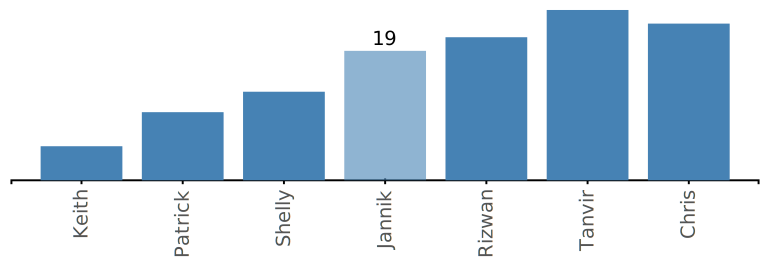
\includegraphics[width=50\respbarwidth]
{diagrams/resp-bar-2.pdf}%
\label{fig:RespBarExample2}%
}
\hfill
\subfloat[][%
30rem
]
{%
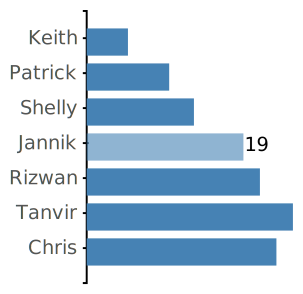
\includegraphics[width=30\respbarwidth]
{diagrams/resp-bar-3.pdf}%
\label{fig:RespBarExample3}%
}
\caption[Responsive Bar Chart Example]
{
A responsive bar chart at different display widths.
\subref{fig:RespBarExample1} At 70rem, axis tick labels are aligned
horizontally. \subref{fig:RespBarExample2} At 50rem, axis tick labels
are aligned vertically. \subref{fig:RespBarExample3} At 30rem, the
chart is transposed.
\imgcredit{Screenshots of \textcite{RespVisPage} created by the author of
  this thesis. Used with kind permission by Keith Andrews.}
}
\label{fig:RespBarExample}
\end{figure}






\subsection{Line Charts}
\label{sec:LineChartExamples}

Line charts are used to show trends in two-dimensional
datasets by plotting them as points connected by lines (a polyline).
They can be extended to compare trends in an additional categorical
dimension by drawing additional polylines for each category. Many line
charts on the web are published in non-responsive forms
\parencite{HLine,HLine2}, although some authors take the extra effort
to make their charts responsive. The minimum which can be done to make
a line chart responsive is to reduce their width
\parencite{RespRadialScatterHLine} on narrower screens by shrinking
the horizontal distance between neighboring points. This usually
occurs together with the recomposition and simplification of
horizontal ticks. If the chart contains annotations, it may also be
necessary to recompose, relocate, and simplify them as well
\parencite{RespHLines,RespHLine,RespHBarHLine,RespHLineHStackedBar}.

A good demonstration of which responsive patterns can be applied to
make a line chart responsive is shown in the responsive line chart
created by \textcite{RespVis} which can be seen in
Figure~\ref{fig:RespLineExample}. In addition to the recomposition of
ticks, tick labels are rotated to reduce their required horizontal
space. For exceptionally limited space, it can make sense to remove
the axes of a line chart entirely and turn it into a sparkline.
However, it should be noted that by doing this, the consumer of the
visualization loses information about the type and scale of the
chart's dimensions. This technique should therefore only be applied in
cases where no other pattern is applicable or if the trend in the data
is the most important message to convey. It is rare to encounter
transposed versions of line charts, although transposition could
sometimes benefit heavily annotated line charts \parencite{VLine}.
Applying a transpose pattern would allow the chart to take up as much
vertical space as necessary to neatly accomodate annotations without
requiring the consumer to scroll horizontally.



\begin{figure}[tp]
\newlength{\resplinewidth}
\setlength{\resplinewidth}{1.15mm}
\centering
\subfloat[][%
65rem
]
{%
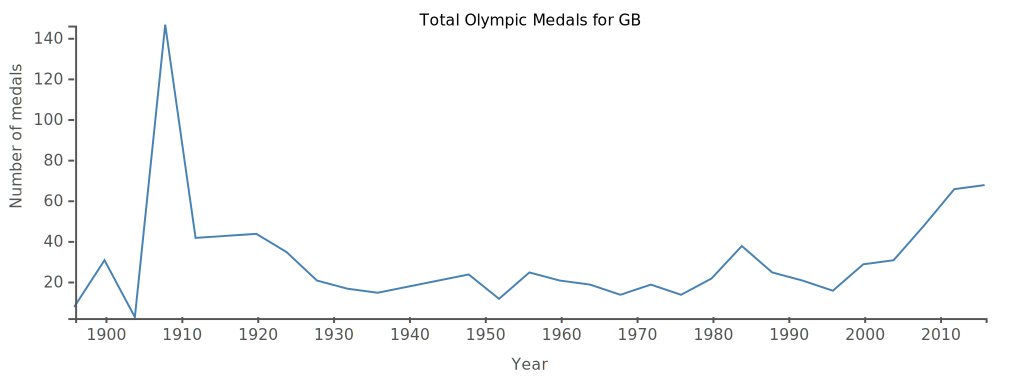
\includegraphics[width=65\resplinewidth]
{diagrams/resp-line-1.pdf}%
\label{fig:RespLineExample1}%
}
\hfill
\subfloat[][%
40rem
]
{%
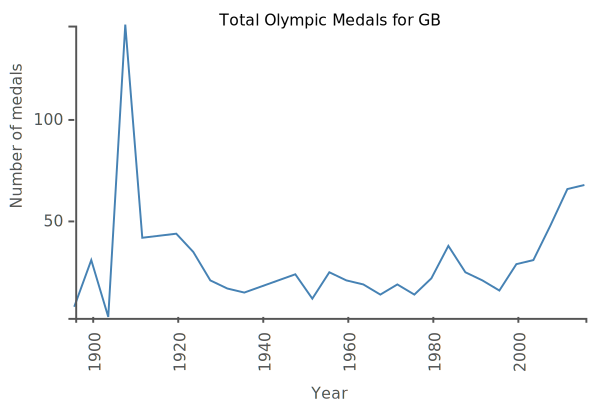
\includegraphics[width=40\resplinewidth]
{diagrams/resp-line-2.pdf}%
\label{fig:RespLineExample2}%
}
\hfill
\subfloat[][%
20rem
]
{%
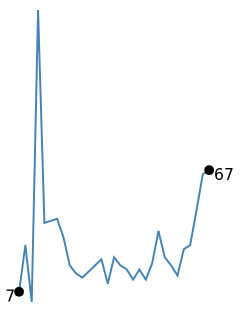
\includegraphics[width=20\resplinewidth]
{diagrams/resp-line-3.pdf}%
\label{fig:RespLineExample3}%
}
\caption[Responsive Line Chart Example]
{
A responsive line chart at different display widths.
\subref{fig:RespLineExample1} At 65rem, the x axis labels are
horizontal.  \subref{fig:RespLineExample2} At 40rem, the x axis ticks
have been thinned out and the labels fully rotated by 90\textdegree.
\subref{fig:RespLineExample3} At 20rem, both axes have been removed,
and the chart has become a sparkline.
\imgcredit{Screenshots of \textcite{RespVisPage} created by the author of
  this thesis. Used with kind permission by Keith Andrews.}
}
\label{fig:RespLineExample}
\end{figure}









\subsection{Point Charts}
\label{sec:ScatterplotExamples}

Point charts, also known as scatterplots, represent data as points in
2d Cartesian coordinate systems. There are many examples of
point charts published as static images \parencite{Scatter,Scatter2},
with responsive versions starting to emerge. The first step to making
point charts responsive is to reduce their width to fit them into the
space available. As for other types of charts, care must be taken to
avoid overlapping of labels and annotations by applying recomposition,
relocation and simplification patterns
\parencite{RespScatter,RespScatter2}. To counteract the increased
density of points when reducing the size of their container, various
interaction features are usually implemented in point charts to aid
consumers in interpreting the represented data. The most useful
interaction features in these charts are elaborative zooming
interactions and the explorative panning interactions. In addition to
zooming and panning, \textcite{RespVis} employs additional methods to
ameliorate the overlapping of individual points, including fisheye
distortion, Cartesian distortion, and temporary displacements of
points.

An interesting technique for responsive point charts based on the
visualization's density (data points per pixel) rather than its width
was introduced by \textcite{NickRabinowitzRDV}. The benefit of this
approach is that charts adapt to changing amounts of data and
reconfigure their appearance accordingly. The patterns applied in the
responsive point chart shown in Figure~\ref{fig:RespScatterExample}
are the recomposition of annotations to only show annotations for
selected data records, and the switching of the encoding from a point
chart to a heatmap for high point densities. Other techniques, such as
the recomposition of data records, would also be applicable to
responsive point charts, but no examples for such patterns could be
found. If the data to be encoded is inherently cyclic, a radial point
chart, using polar coordinates, can be used to better reflect the
cyclic nature of the data \parencite{RespRadialScatterHLine}.



\begin{figure}[tp]
\centering
\subfloat[][%
Low density % (0.00005 points per pixel).
]
{%
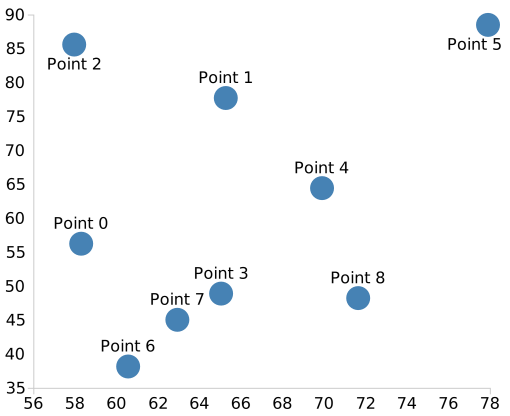
\includegraphics[width=0.3\linewidth]
{diagrams/resp-scatter-1.pdf}%
\label{fig:RespScatterExample1}%
}
\hfill
\subfloat[][%
Medium density % (0.0007 points per pixel).
]
{%
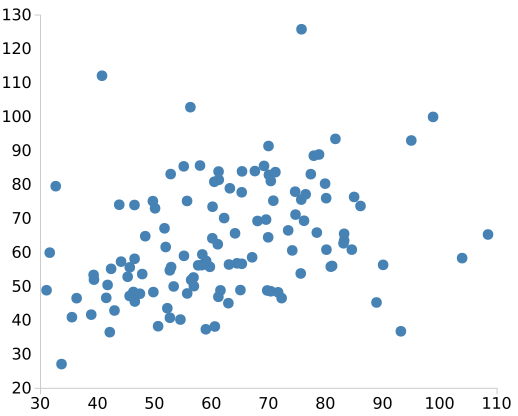
\includegraphics[width=0.3\linewidth]
{diagrams/resp-scatter-2.pdf}%
\label{fig:RespScatterExample2}%
}
\hfill
\subfloat[][%
High density % (0.017 points per pixel).
]
{%
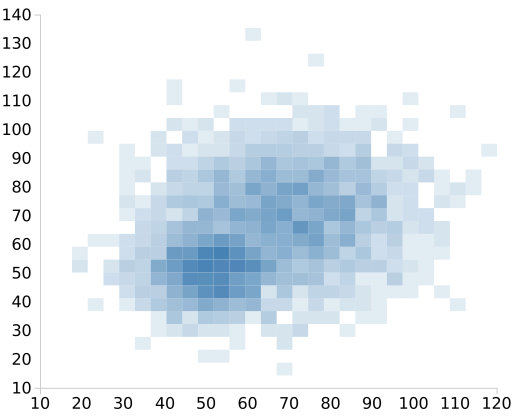
\includegraphics[width=0.3\linewidth]
{diagrams/resp-scatter-3.pdf}%
\label{fig:RespScatterExample3}%
}
\caption[Responsive Point Chart Example]
{
A responsive point chart based on data density (data
points per pixel). \subref{fig:RespScatterExample1} With a small
number of data points, all points and their corresponding labels are
shown. \subref{fig:RespScatterExample2} At a certain density, labels
are only shown for selected points. \subref{fig:RespScatterExample3}
At very high densities, the point chart is replaced by a heatmap to
more efficiently display the large amount of data.
\imgcredit{Screenshots created by the author of this thesis.
Visualization created by \textcite{NickRabinowitzRDV}}
}
\label{fig:RespScatterExample}
\end{figure}


\subsection{Parallel Coordinates}

Even though parallel coordinates charts
\parencite{ParallelCoordinates} are rarely encountered in
non-technical contexts, they are quite popular when it comes to
visualizing multidimensional data in visual analytics systems
\parencite{HighD}. In these kinds of charts, multiple dimensions are
rendered as parallel axes, upon which points are connected via paths
(polylines). Each polyline represents a data record and its values at
the corresponding dimensions. The axes of a parallel coordinates chart
are typically laid out horizontally, meaning that the chart can be
made narrower by reducing the distance between individual axes.
Previously mentioned axis-related responsive patterns, such as
rotating labels and recomposing ticks, can also be applied.

Another technique is to temporarily hide some dimensions, based on
some criteria. When automatically hiding dimensions, it is necessary
to apply compensation patterns, giving the user additional controls to
configure which dimensions are displayed and override the system's
hiding behavior. An example of a responsive parallel coordinates chart
incorporating some of these patterns can be seen in
Figure~\ref{fig:RespParCoordExample}.
%
If reducing the chart's complexity is not appropriate, an alternative
is to transpose the chart, so its dimensions are laid out vertically
and vertical scrolling can be used to explore the full chart.




\begin{figure}[tp]
\newcommand{\respparcoordscale}{0.36}
\centering
\subfloat[][%
61rem
]
{%
\includegraphics[valign=b,scale=\respparcoordscale]
{images/resp-parcoord-1.png}%
\label{fig:RespParCoordExample1}%
}
\hfill
\subfloat[][%
50rem
]
{%
\includegraphics[valign=b,scale=\respparcoordscale]
{images/resp-parcoord-2.png}%
\label{fig:RespParCoordExample2}%
}
\newline
\subfloat[][%
40rem
]
{%
\includegraphics[valign=b,scale=\respparcoordscale]
{images/resp-parcoord-3.png}%
\label{fig:RespParCoordExample3}%
}
\hfill
\subfloat[][%
30rem
]
{%
\includegraphics[valign=b,scale=\respparcoordscale]
{images/resp-parcoord-4.png}%
\label{fig:RespParCoordExample4}%
}
\hfill
\subfloat[][%
30rem, user-configured dimensions
]
{%
\includegraphics[valign=b,scale=\respparcoordscale]
{images/resp-parcoord-5.png}%
\label{fig:RespParCoordExample5}%
}
\caption[Responsive Parallel Coordinates Chart Example]
{
A responsive parallel coordinates chart at different display widths.
\subref{fig:RespParCoordExample1} At larger widths, all dimensions are
shown. \subref{fig:RespParCoordExample2} Dimensions are removed based
on their priority, dimension labels are rotated by 45 degrees, and a
dimensions toggle is shown which enables the configuration of
dimensions. \subref{fig:RespParCoordExample3} Further dimensions are
removed. \subref{fig:RespParCoordExample4} Further dimensions are
removed, and dimension labels are rotated by 90 degrees.
\subref{fig:RespParCoordExample5} The dimension configuration panel
has been opened, and the user has taken control over which dimensions
to show.
\imgcredit{Screenshots of \textcite{RespVisPage} created by the author of this thesis.
Used with kind permission by Keith Andrews.}
}
\label{fig:RespParCoordExample}
\end{figure}

       

\cleardoublepage

\chapter{The RespVis Library}
\label{chap:RespVis}

RespVis is an open-source D3 extension library for creating responsive
SVG charts \parencite{RespVisGitHub,RespVisLive}. It enables the use
of CSS for the responsive styling and layout of
visualizations. RespVis renders visualizations as pure and complete
SVG documents, meaning that the whole visualization is contained in
one SVG document and includes no elements of other XML namespaces.
RespVis is designed as an extension to D3, rather than a wrapper
around it. Unlike most other visualization libraries built on top of
D3, RespVis does not hide D3 behind a custom API. Rather,
visualization authors invoke RespVis functionality by binding
specially structured data to D3 Selections, which render visualization
components using render functions to transform the bound data into
some form of visual representation. Furthermore, RespVis espouses the
strong separation between data and code and applies strong static
type-checking through the use of TypeScript.






\section{Design}
\label{sec:Design}

The design of the RespVis library is guided by six principles:
\begin{enumerate}
\item Style and Layout via CSS.
\item Pure and Complete SVG Documents.
\item Extend D3.
\item Separate Data and Code.
\item Strong Static Type-Checking with TypeScript.
\item Layered Component Hierarchy.
\end{enumerate}




\subsection{Style and Layout via CSS}

Every part of a visualization that can be configured with CSS should
be configured with CSS. The visual appearance and layout of HTML
elements can already be configured by CSS. Many presentation
attributes of SVG elements can also be styled with CSS. However,
CSS-based layouting cannot be applied to SVG elements, which seriously
limits the responsive capabilities of using CSS for SVG charts.
Without powerful CSS layout technologies like Flexbox and Grid, all
the individual components of an SVG chart have to be positioned
manually via JavaScript.

The RespVis Layouter enables the layouting of visualization components
using powerful standard CSS-based layout mechanisms such as Flexbox
and Grid, by calculating the bounding boxes of SVG elements from the
CSS configuration of a shadow \elname{<div>} hierarchy. The Layouter
offers visualization authors comparable configurability to what they
are used to when laying out HTML elements. For example, a legend can
be configured to be placed to the right of a chart in a wider view,
and beneath the chart in a narrower view, using familiar CSS
constructs.





\subsection{Pure and Complete SVG Documents}

Every RespVis visualization should be rendered as a pure and complete
SVG document. An SVG document is considered \emph{pure}, if it
contains only elements defined in the SVG namespace. This means that
it must not contain any \elname{<foreignObject>} elements, which embed
elements of an XML namespace other than SVG, for example to embed HTML
elements inside an SVG. RespVis does not support rendering to HTML
canvas elements, because graphics rendered there cannot be styled by
CSS.

An SVG document representing a visualization is considered
\emph{complete}, if it contains the entire visualization within
it. Splitting visualization components across multiple SVG documents
is considered bad practice, because these components conceptually
belong together and should be represented as a whole. Having
a full visualization enclosed in a complete SVG document allows the
whole visualization to be exported and stored as a standard-compliant
SVG file, which can be further processed using a wide range of tools.




\subsection{Extend D3}

RespVis is designed as a library which extends D3, rather than a
wrapper around D3. Compared to other visualization libraries which
wrap a layer around D3, it does not provide an entirely new interface
to visualization authors, but uses D3 Selections as the core interface
with which to interact. The typical workflow of invoking RespVis
functionality is to bind data objects of a specific structure to the
elements of a Selection and then to visualize this data by calling a
render function to transform it into visual marks. If D3 were hidden
behind a custom API, its powerful capabilities would not be directly
accessible to users of the library, and would need to be exposed
manually through special mechanisms. By designing RespVis as an
extension of D3, visualization authors can continue to leverage its
expressive and concise API and author their documents using data joins
and the general update pattern.



\subsection{Separate Data and Code}

In RespVis, data and code are decoupled from each other. Everything in
RespVis is built from functions and objects without using any classes.
Classes were avoided, since they are not common when working with D3,
and also because they lead to a tight coupling between data and
functionality, which was deemed undesirable. The decoupling of data
and code results in various benefits compared to the prevalent
object-oriented way of building software. Among these benefits are
easier reuse and testing of functions and a software system which
requires less cognitive effort to understand.

Functions are easier to reuse because they only require well-shaped
input data to perform their task. Mechanisms like inheritance or
composition, which tend to increase the complexity of a system, are
unnecessary. Compared to class-based code, where an object needs to be
instantiated before testing its methods, it is easier to test
functions in isolation when they are not coupled to their data. The
reason for this is that the instantiation of an object might be a
complex operation dependent on other methods which could affect the
results of a test case.

Possibly the main benefit of decoupling data and code lies in the
reduced complexity of the resulting system. A software system which
treats data and code as different entities might be composed of more
entities than a system which does not, but the individual entities
have fewer dependencies between one another. The reduced number of
dependencies between entities results from separating entities into a
data entities group and a function entities group, with no
relationships between them. The research related to software
complexity is hard to convey in simple terms, but one rule of thumb is
well summarized by \textcite{DataCodeSeparation} as \enquote{A system
  made of disjoint simple parts is less complex than a system made of
  a single complex part.} Of course, there are also drawbacks when
designing a system adhering to this concept, but they are not too
severe and are therefore not listed here. For further reading on this
topic, the reader is directed to Moseley and Marks' classic workshop
paper \parencite{OutOfTarPit} and Sharvit's forthcoming book
\parencite{Sharvit-Book}.




\subsection{Strong Static Type-Checking with TypeScript}

The RespVis library is written in TypeScript, with everything being as
strongly-typed as possible. For the most part, interfaces are used to
describe the structure of data objects, and function parameters are
annotated with types. Whenever working with D3 Selections, their
contents are typed as strongly as possible using the generic type
variables available on Selections. Most of the time, it is sufficient
to specify only the type of elements contained in a Selection and the
structure of the data bound on them. If the element and data types of
a Selection are declared, the various functions can assume that
parameters passed to them have specific types, and they do not have to
worry about dynamic type checking. Applying a strongly typed system
has many advantages, such as better development tooling and
compile-time identification of type-related bugs. These advantages are
described in Section~\ref{sec:TS}.







\subsection{Layered Component Hierarchy}

Components in RespVis are structured in four layers with increasing
levels of abstraction, as shown in Figure~\ref{fig:Layers}. Components
in higher layers make more assumptions about their content than
components in lower layers. The bottom-most layer with the lowest
level of abstraction consists of visual Primitives, represented by
basic SVG elements like \elname{<rect>}, \elname{<circle>}, and
\elname{<text>}. These Primitives do not require any data to be bound to
them and are simply rendered by setting their attributes to the
desired values.


\begin{figure}[tp]
\centering
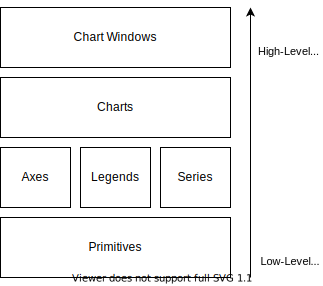
\includegraphics[keepaspectratio,width=\linewidth,height=7.5cm]
{diagrams/respvis-layers.pdf}
\caption[Component Layers of RespVis]{
The four layers of components in the RespVis library. Higher layers
contain increasingly higher-level components.
\imgcredit{Image created by the author of this thesis.}
}
\label{fig:Layers}
\end{figure}


The second layer comprises composite components such as Axes, Legends,
and Series. These are usually rendered as \elname{<svg>} or \elname{<g>}
elements containing only primitive elements. The components in this
layer are the lowest-level components which are configured using
structured data bound to their elements. Series components are
composite elements which render a collection of underlying elements
using a data join and the general update pattern.

The third layer consists of Chart components. Charts are composite
components which can also include other composite components. They are
the visual entities which represent complete visualizations and are
usually composed of axes, series, and legends.

In many other visualization libraries, charts are the highest-level
components visualization authors can work with, but RespVis contains
an additional layer above them, formed by Chart Window components.
Chart Windows are wrapper components around Charts. Unlike the
previously discussed lower layers, Chart Windows are not rendered as
SVG elements but as HTML \elname{<div>} elements. Their purpose is to
nest Charts into a Layouter component, render them in a three-phased
rendering process, and provide an optional toolbar for them. Toolbars
are customizable and can hold different tools for different types of
chart.








\section{Naming Conventions}
\label{sec:NamingConventions}

The naming of entities in RespVis follows the same naming conventions
used in D3 modules. The names of entities usually start with the name
of the group to which an entity belongs and are then further narrowed
down by successively adding more words until the exact entity is
accurately described. This convention is referred to as
\enquote{top-down naming} in this thesis. An example of the top-down
naming convention can be seen in the D3 Scale
\parencite{D3Scale} and D3 Axis \parencite{D3Axis} packages, in
which entities are called things like \code{scaleLinear},
\code{scaleOrdinal}, \code{axisBottom}, and \code{axisLeft} rather
than \code{linearScale}, \code{ordinalScale}, \code{bottomAxis}, and
\code{leftAxis}. Since this is the exact opposite of how these
entities would be called in natural English, using such names
can feel odd for the uninitiated. However, experience shows working
with APIs which follow such a naming convention is easier than with
those which do not, since users of such APIs can easily discover
specialized entities by inputting the general entity type and browsing
through code completion suggestions provided by their development
tools. Hence, entity names in RespVis also follow this convention.

The RespVis public interface is made up of types and functions. Types
are usually written as interfaces and represent the shape of an
object. Type names are written in \code{PascalCase}
\parencite{PascalCase} and adhere to the top-down naming
convention. They always start with the group a type belongs to, and
further words are appended to distinguish ever more specialized
types. The naming of types can best be demonstrated by the different
names given to interfaces describing data objects to configure
different kinds of Bar Charts. Data objects for the configuration of
Basic Bar Charts are described by the \code{ChartBar} interface, those
of Grouped Bar Charts are described by the \code{ChartBarGrouped}
interface, and those of Stacked Bar Charts are described by the
\code{ChartBarStacked} interface.

The API of RespVis is largely composed of functions. Function names
are always written in \code{camelCase} \parencite{camelCase} and also
follow the top-down naming convention. Function names always start
with the type of object on which they operate, followed by the
operation they perform. A component in RespVis always consists of a
data object which describes it, an element to which the data object is
bound, and a render function which transforms the bound data into some
form of visual representation. The names of functions to create data
objects for the configuration of components are always in the form of
\code{componentNameData}, such as \code{chartBarData} or
\code{chartBarGroupedData}. Functions which transform bound data into
a visual representation are always named in the form of
\code{componentNameRender}, such as \code{chartBarRender} or
\code{chartBarGroupedRender}.






\section{Project Structure}
\label{sec:ProjectSetup}

RespVis is a NodeJS \parencite{NodeJS} project hosted as an
open-source project on GitHub \parencite{RespVisGitHub}. It is
implemented in TypeScript and grouped into different packages by
thematic affinity. The TypeScript source files are compiled
(transpiled) to JavaScript and bundled into one combined library
package, which visualization authors can then import into their
projects.
%
The Rollup module bundler \parencite{Rollup} is used to perform
compilation and bundling. In addition to the bundled JavaScript
library, visualization authors are required to import an accompanying
CSS file containing default styling for the generated visualizations.
The project also contains examples demonstrating usage of the library
to create various charts. These examples are HTML files which import
the required files and contain JavaScript to invoke RespVis
functionality to create and update visualizations.
%
The Gulp \parencite{Gulp} task runner is used to automate the build
process of the library, including the preparation of the output
directory, the bundling of library code, and the copying of various
files to the correct locations in the output directory.




The RespVis project contains configuration files for various tools, a
\code{src/} directory containing the source code for the whole library
and accompanying examples, a \code{node_modules} directory containing
the project's cached NodeJS dependencies, and a \code{dist/} directory
containing built versions of the library and examples ready for
distribution. The configuration files are only discussed broadly here,
later sections go into more detail about the setup of the various
tools. An overview of the most important files and directories can be
seen in Figure~\ref{fig:RespVisDirTree}.

\begin{figure}[tp]
\centering
\framebox[\textwidth]{%
\begin{minipage}{0.9\textwidth}
\begin{footnotesize}
  \dirtree{%
  .1 /.
  .2 dist/.
  .3 examples/.
  .4 data/.
  .4 vendor/.
  .4 bar.html.
  .4 \dots.
  .3 index.html.
  .3 respvis.css.
  .3 respvis.[m]js.
  .3 respvis.[m]js.map.
  .3 respvis.min.[m]js.
  .3 respvis.min.[m]js.gz.
  .3 respvis.min.[m]js.map.
  .2 node\_modules.
  .2 src/.
  .3 lib/.
  .4 bars/.
  .4 core/.
  .4 legend/.
  .4 lines/.
  .4 points/.
  .4 tooltip/.
  .3 examples/.
  .4 data/.
  .4 vendor/.
  .4 bar.html.
  .4 \dots.
  .3 index.html.
  .3 respvis.css.
  .2 gulpfile.js.
  .2 package.json.
  .2 tsconfig.json.
  }
\end{footnotesize}
\end{minipage}
}
\caption[RespVis Directory Structure]{
  The most important files and directories of the RespVis project. 
  \imgcredit{Figure created by the author of this thesis.}
}
\label{fig:RespVisDirTree}
\end{figure}



The root directory of the RespVis project contains the necessary
project configuration files for NodeJS, TypeScript, and Gulp. The
NodeJS configuration file, \code{package.json}, describes the
meta-data of the NodeJS package. It is used to specify the project's
dependencies to other packages, and is required for every NodeJS
package, so that it can be uploaded to the npm package registry
\parencite{npm}. The TypeScript configuration file,
\code{tsconfig.json}, specifies the configuration the TypeScript
compiler uses to compile the library's TypeScript source files into
their JavaScript counterparts. The Gulp configuration file,
\code{gulpfile.js}, is used to describe atomic, recurring tasks and
compositions of them. These tasks can then be invoked via the Gulp
command-line tool to automate otherwise tedious workflow processes.

The \code{src/} directory at the root of the project contains all the
implementation files of the library in the \code{src/lib/} directory
and examples in the \code{src/examples/} directory. The
\code{src/lib/} directory contains all TypeScript source files of the
library. They are partitioned into packages formed around the thematic
affinity of the various components. The Core package
contains the core functionality of the library and is a prerequisite
for all the other packages. It includes the Layouter, Chart base
functionality, Chart Window base functionality, and various utility
functions. The Legend package contains modules to render
legends consisting of a title and configurable labeled symbols. The
Tooltip package contains functions to show and hide
tooltips, modify their contents, and position them. It also contains
helper functions for Series to prevent the replication of
tooltip-related code in their data creation and rendering functions.
The Bars, Lines, and Points packages
contain the necessary modules to render Series, Charts, and Chart
Windows for bar, grouped bar, stacked bar, line, and point
visualizations. At the moment, all these packages are built into a
combined one, but there are plans to also distribute them separately
to allow users of the library to import only the packages they need.

The \code{src/examples/} directory holds the source files of the
developed examples. These examples are distributed alongside the
library files, and are copied over to the \code{dist/examples/}
directory when building the project. Every example consists of an HTML
file which imports all the requirements such as \code{respvis.js} and
\code{respvis.css} as well as external dependencies such as D3. It
then invokes the necessary RespVis functionality within a
\elname{<script>} tag embedded in the body of the HTML document. In
addition to individual example files, the \code{examples} directory
also contains a \code{vendor} directory, which contains third-party
dependencies, and a \code{data} directory containing data imported by
individual examples.

In addition to configuration files and the \code{src/} directory, the
root directory also contains two directories which are automatically
generated during the build process. These are the \code{node_modules/}
and \code{dist/} directories. The \code{node_modules/} directory
exists in every NodeJS package. It is created when installing the
dependencies of a package and contains a cached copy of every
direct and indirect dependency. The \code{dist/} directory is
generated by the Gulp build tasks and contains all the files necessary
to distribute a built version of the RespVis library.

The code of the RespVis library is distributed as JavaScript bundles
in both the older IIFE (Immediately Invoked Function Expressions)
format and the more modern ES modules format. These formats are
explained in more detail in Section~\ref{sec:Rollup}. Bundles
containing the \code{.js} extension in their file name contain IIFE
source code, whereas bundles containing the \code{.mjs} extension
contain ES module source code. Furthermore, these bundles are also
distributed in minimized versions. The \code{dist/respvis.[m]js} file
contains the unmodified JavaScript bundle that can be used by library
consumers who require readable code, \code{dist/respvis.min.[m]js}
contains the minified JavaScript bundle, and
\code{dist/respvis.min.[m]js.gz} contains the minified JavaScript
bundle that has additionally been compressed in the GZIP format
\parencite{GZIP}. Alongside these code bundles, Rollup creates source
maps for the \code{dist/respvis.[m]js} and
\code{dist/respvis.min.[m]js} bundles: \code{dist/respvis.[m]js.map}
and \code{dist/respvis.min.[m]js.map}, respectively. These source maps
are interpreted by developer tools in browsers to map from certain
instructions in the bundled JavaScript code to the exact instruction
in the original TypeScript code and are immensely helpful for
debugging.


Since RespVis aims to perform all possible styling in CSS, the
distribution also contains a \code{dist/respvis.css} file with the
default styles for visualizations created with RespVis. Currently,
this file is written manually as a whole in the \code{src/} directory
and merely copied to the \code{dist/} directory during the build
process. In the future, this process could be improved by employing a
CSS preprocessing tool such as SASS \parencite{SASS}, so that the
styles can be split into multiple files during development. Besides
the bundled library source code and stylesheet, the \code{dist/}
directory also contains usage examples of RespVis in the
\code{dist/examples/} directory, copied over from the
\code{src/examples/} directory.






\section{NodeJS}

NodeJS is a standalone JavaScript runtime \parencite{NodeJS}, built on
top of the V8 JavaScript engine \parencite{V8}, which is an
open-source and multi-platform runtime for the execution of JavaScript
code. NodeJS allows JavaScript code to be run outside of web browsers.
NodeJS is heavily used for server-side development to unify the
technology stack of web developers and allow them to use JavaScript
for both client-side and server-side development. However, with the
appropriate project setup, NodeJS can be used for any kind of
development, and it can be set up as a powerful framework to develop
client-side applications as done in this project. One of the most
important tools in the NodeJS environment is the npm package manager
\parencite{npm}, which exists to simplify the sharing of packages and
their dependency management. The npm package registry hosts a huge
number of packages that can easily be imported and used to create new
ones.

RespVis is developed as an npm package. Every npm package is
configured via a \code{package.json} file. This file contains all the
necessary meta-data for a package to make it identifiable and provide
information about what the package contains. The \code{package.json}
file also lists all the dependencies of a package, so they can
automatically be updated and downloaded during an installation
process. A package can rely upon both normal dependencies and
development dependencies. Normal dependencies of a package are
required for it to work at run time and need to be installed alongside
it. Development dependencies are only required during development and
are only installed when installing a local package. The
\code{package.json} file is located in the root directory of the
RespVis package and can be seen in Listing~\ref{list:PackageJSON}.


\begin{samepage}
\lstinputlisting[%
  float=tp,
  aboveskip=\floatsep,
  belowskip=\floatsep,
  xleftmargin=0cm,              % no extra margins for floats
  xrightmargin=0cm,             % no extra margins for floats
  %
  basicstyle=\footnotesize\ttfamily,
  frame=shadowbox,
  numbers=left,
  label=list:PackageJSON,
  caption={[RespVis \code{package.json} File]%
    The \code{package.json} file of the RespVis library.
    This file contains all the meta-data describing the package and its dependencies.
    Keywords and type dependencies have been omitted for readability.
  },
]{listings/package.json}
\end{samepage}






\section{Rollup}
\label{sec:Rollup}

The Rollup module bundler \parencite{Rollup} is used to bundle the
source code of the RespVis library into bundles of different
kinds. Bundling combines code written as multiple smaller modules into
one combined package to make it easier to distribute. Developers do
not have to worry about the details of how their code will be
packaged, as Rollup takes care of all the necessary
transformations. In addition to bundling source code, Rollup also
performs \emph{tree shaking} on the bundled code, eliminating unused
code from the resulting bundle by statically analyzing dependencies
between modules.
%
Rollup supports the creation of bundles in several common module
formats, such as CommonJS, Asynchronous Module Definition (AMD),
Universal Module Definition (UMD), Immediately Invoked Function
Expressions (IIFE), and ES. RespVis is distributed as both IIFE and ES
modules.

IIFE modules have been used for a long time. They were used to support
modular software designs in JavaScript before more elaborate module
formats were defined. IIFE modules are anonymous functions which are
executed directly after declaring them. These functions contain the
full logic of the module and return an object representing its
publicly accessible interface. This object is usually stored in a
variable to allow interaction with the module after its creation.
IIFE modules are plain JavaScript and do not require any modern
features to be supported by browsers. They are simply loaded into web
documents like any other JavaScript resource via a \elname{<script>}
element. The example in Listing~\ref{list:IIFE} illustrates the IIFE
module format.



\begin{samepage}
\lstinputlisting[%
  float=tp,
  aboveskip=\floatsep,
  belowskip=\floatsep,
  xleftmargin=0cm,              % no extra margins for floats
  xrightmargin=0cm,             % no extra margins for floats
  %
  basicstyle=\footnotesize\ttfamily,
  frame=shadowbox,
  numbers=left,
  label=list:IIFE,
  caption={[IIFE Module Format]%
IIFE (Immediately Invoked Function Expression) modules wrap the module
code inside a function, which is executed immediately after declaring it
and returns the public interface of the module.
\code{do-something.js} contains the original code that should be
wrapped as an IIFE module, \code{module.js} contains the code of the
IIFE module, and \code{application.js} demonstrates usage of the
module.
},
]{listings/iife.js}
\end{samepage}



ES modules are a more recent addition to JavaScript, introduced in
ECMAScript 6 \parencite{ECMAScript6}. They are a native module system
built around the \code{import} and \code{export} statements, which are
widely supported by modern browsers. Since the individual modules of
the RespVis library are built as ES modules anyway, Rollup mostly only
has to merge them to create a valid, combined ES module. ES modules
are natively supported in browsers, so they can be loaded directly in
a HTML document using a \elname{<script>} element. However, it is
necessary to mark them as modules by setting the \attrname{type}
attribute to \code{module} on the loading \elname{<script>} element,
so that browsers can interpret them accordingly.


The core package of Rollup is only able to create mostly unmodified
bundles from JavaScript source files. Various plugins add
frequently required additional functionality. There are two kinds of
Rollup plugins: bundle plugins, which affect the bundling process, and
output plugins, which transform the already bundled code.

The Rollup bundle plugins used for the bundling of RespVis are
\code{@rollup/plugin-node-resolve}, \code{@rollup/plugin-commonjs},
and \code{@rollup/plugin-typescript}. The
\code{@rollup/plugin-node-resolve} plugin is used to resolve imports
from other NodeJS packages that reside in the \code{node_modules}
directory. Since many NodeJS packages are still implemented as
CommonJS modules, which are not natively supported by Rollup, the
\code{@rollup/plugin-commonjs} plugin is used to interpret them.
Lastly, the \code{@rollup/plugin-typescript} plugin is used to compile
TypeScript source files to JavaScript before bundling them. The
configuration for the TypeScript compiler is taken from the
\code{tsconfig.json} file at the root directory of the project.

The Rollup output plugins used during the bundling process are
\code{rollup-plugin-terser} and \code{rollup-plugin-gzip}. These
plugins do not affect every created bundle, but are used to
selectively transform the contents of specific bundles. The
\code{rollup-plugin-terser} plugin is used to create minified versions
of the RespVis bundles denoted by the term \code{.min} in their file
names. Logically, they are the same as the equivalent unminified
bundles, but are compressed as much as possible to reduce their file
size while still containing valid, but unreadable, JavaScript
code. The \code{rollup-plugin-gzip} plugin is used to create
compressed gzipped versions of the RespVis bundles denoted by the term
\code{.gz} in their file extensions \parencite{GZIP}.

Note that D3 is not included in any of the generated RespVis
bundles. RespVis is designed to be an extension of D3 and, most of the
time, an application wishing to use RespVis will already be using
D3. If D3 were to be included in the RespVis bundle, it would
unnecessarily be loaded a second time. To prevent D3 from being
included in the created bundles, all dependencies on D3-related
packages are marked as external.

The actual bundling is performed via the JavaScript API of Rollup in
the private \code{bundleJS} Gulp task. This task is executed in
various automation processes set up with Gulp, which are explained in
more detail in Section~\ref{sec:Gulp}. The code of the \code{bundleJS}
task can be seen in Listing~\ref{list:BundleJS}. The RespVis library
is bundled via the \code{Rollup.rollup} function which returns the
created bundle. This bundle is then written to one or more target
destinations via the \code{Bundle.write} method, which allows the
specification of the target bundle format and any plugins used to
transform the code before writing it.


\begin{samepage}
\lstinputlisting[%
  float=tp,
  aboveskip=\floatsep,
  belowskip=\floatsep,
  xleftmargin=0cm,              % no extra margins for floats
  xrightmargin=0cm,             % no extra margins for floats
  basicstyle=\footnotesize\ttfamily,
  frame=shadowbox,
  numbers=left,
  label=list:BundleJS,
  caption={[Gulp Task to Bundle RespVis]%
The private Gulp task which bundles the code of the RespVis libary.
The bundle is created once and then written to multiple targets.
}
]{listings/bundle-js.js}
\end{samepage}
  





\section{Gulp}
\label{sec:Gulp}

Gulp is a task runner which automates workflow processes via a set of
named tasks \parencite{Gulp}. It is used to automate processes like
building the library and serving examples on a development server.
Tasks are useful for automating operations which need to be carried
out repeatedly. They can perform an atomic operation or be composed of
other tasks. Composite tasks can execute tasks contained in them in
serial or in parallel. The tasks are implemented as JavaScript
functions in the Gulp configuration file, \code{gulpfile.js}, which
can be found in the root directory of the project. Gulp's approach of
favoring code over declarative configuration files means that the
person setting up process automation needs to be familiar with
JavaScript. In return, the possibilities for configuration are
endless.

Tasks in the \code{gulpfile.js} file are separated into private and
public tasks. Private tasks are simply asynchronous functions which
perform a certain action that does not necessarily have to be executed
by external entities. The private tasks in the RespVis project are
\code{bundleJS}, \code{bundleCSS}, \code{copyExamples},
\code{cleanDist}, \code{cleanNodeModules}, and \code{reloadBrowser}.
%
Public tasks are also asynchronous functions, but they are exported
and are therefore available to be executed via the Gulp command-line
interface. Most public tasks in the RespVis project are compositions
of other tasks. The public tasks in RespVis are \code{clean},
\code{cleanAll}, \code{build}, and \code{serve}. The default task,
\code{serve}, is executed when no other task is specified on the
command line. A hierarchical representation of all the tasks in the
\code{gulpfile.js} file is shown in Listing~\ref{list:GulpTasks}.

\begin{samepage}
\lstinputlisting[%
  float=tp,
  aboveskip=\floatsep,
  belowskip=\floatsep,
  xleftmargin=0cm,              % no extra margins for floats
  xrightmargin=0cm,             % no extra margins for floats
  %
  basicstyle=\footnotesize\ttfamily,
  frame=shadowbox,
  numbers=left,
  label=list:GulpTasks,
  caption={[Tasks Defined in \code{gulpfile.js}]%
A hierarchical representation of the tasks defined in the \code{gulpfile.js} file,
as output by the \code{gulp --tasks} command.
},
]{listings/gulp-tasks.txt}
\end{samepage}
  


Bundling the RespVis library's source code is implemented in the
private \code{bundleJS} task. It uses the JavaScript API of Rollup to
compile the TypeScript source files into JavaScript and bundle them
into IIFE and ES modules of varying levels of minification. This task
has already been described in detail in Section~\ref{sec:Rollup}, so
it won't be discussed further here. It is executed during the public
\code{build} and \code{serve} tasks.

The \code{bundleCSS} task is used to copy the \code{src/respvis.css}
file to the \code{dist/} directory. Since one of the design pillars of
RespVis is to style everything possible with CSS, this file contains
all the default styles for visualizations created with
RespVis. Currently, this file is one large single file in the
\code{src/} directory and is merely copied over to the \code{dist/}
directory, but there are plans to build this file from different
modules using a CSS preprocessor in the future, which will require an
additional bundling step. This task is executed as part of the public
\code{build} and \code{serve} tasks.

The private \code{copyExamples} task copies all the files from the
\code{src/examples/} directory to the \code{dist/} directory. This
task is required because the examples are developed inside the
\code{src/} directory, but need to be made available in the
distributable library packages. Another reason for the copying is that
the BrowserSync development server is initialized with the
\code{dist/} directory as its root, and every potentially viewable
file must reside somewhere in that directory. The \code{copyExamples}
task is executed during the public \code{build} and \code{serve}
tasks.

The private \code{cleanDist} and \code{cleanNodeModules} tasks are
used to delete the \code{dist/} and \code{node_modules/} directories,
respectively. The \code{cleanDist} task is additionally exported as
the public \code{clean} task. This task is necessary because without
cleaning the \code{dist/} directory before every rebuild, redundant
files from previous builds that might have disappeared in the meantime
would cause littering and confusion. Therefore, this task is executed
as the first step of the \code{build} task. The public \code{cleanAll}
task is composed of the private \code{cleanDist} and
\code{cleanNodeModules} tasks. It is manually executed by a developer
to delete the currently cached dependencies of the project, to then
reinstall them from scratch.

The public \code{build} task is responsible for building all parts of
the project. It is a composite task which executes the \code{clean},
\code{bundleJS}, \code{bundleCSS}, and \code{copyExamples} tasks. The
\code{clean} task is invoked before all of the other tasks, which are
then executed in parallel. After this task finishes, the \code{dir/}
directory will contain all distributable JavaScript and CSS files of
the library, as well as the distributable \code{examples/} directory.

To simplify the development of RespVis, a Browsersync
\parencite{Browsersync} development server is used to host the built
distributables. Browsersync is a useful tool for synchronized browser
testing during development. It has many features like simulated
network throttling, interaction synchronization, and file
synchronization, which enable simultaneous testing in multiple
environments. For RespVis, it is only used for its ability to
synchronize and hot-reload files on the fly. The public \code{serve}
task, which is also exported as the default task, initializes a
Browsersync development server which serves files from the
\code{dist/} directory. Automatic reloading of the development server
is implemented manually via the \code{Gulp.watch} function. This
function enables a task to be executed whenever a change to a watched
file (matched by the supplied glob pattern) is detected. The
\code{serve} task implements three different cases which cause the
development server to reload. Firstly, every time one of the
TypeScript files in the \code{src/lib/} directory changes, the
\code{bundleJS} task is executed, and the browser is
reloaded. Secondly, every time the \code{src/respvis.css} file
changes, the \code{bundleCSS} task is executed, and the browser is
reloaded. Thirdly, whenever a file in the \code{src/examples/}
directory is changed, the \code{copyExamples} task is executed, and
the browser is reloaded.


     

\cleardoublepage
\chapter{Modules}
\label{chap:Modules}

The source code of RespVis is structured into modules written in the ES module format.
Currently, all these modules are combined into a single, monolithic library bundle during the build process.
In the future, each module will be released on its own to allow users to import only the ones they need.
The reason for this is that most users will likely only require a subset of all the features included in the library and it would unnecessarily increase the size of their bundles to import all of them.
A good example of this is D3, which also separates its considerable amount of features into different modules that can be successively added to a project when the need arises.

At the time of writing, the RespVis library contains five different modules: the core, legend, tooltip, bar, and point modules.
Each of these modules contains submodules that have been grouped by thematic similarity.
The core module holds the core functionality of the library that all other modules depend on, which includes the layouter, axes, chart and chart window base components, and various utility functions and types.
The legend module contains the implementation of a legend component that is mostly meant to describe discrete data dimensions by rendering distinct values as labeled symbols.
The tooltip module holds functions to control the showing, placement, and content of tooltips, as well as utility functions that simplify the configuration and initialization of tooltips on series components.
% None of the modules listed so far contain components that render visual marks, which are characteristic for visualizations.
The bar module distinguishes between normal, grouped, and stacked bars and includes various low-level and high-level components to render each of those types.
Similarly, the point module contains low-level and high-level components to visualize point charts.
All of the different modules and the dependencies between them are shown in Figure~\ref{fig:Modules}.

\begin{figure}[tp]
  \centering
  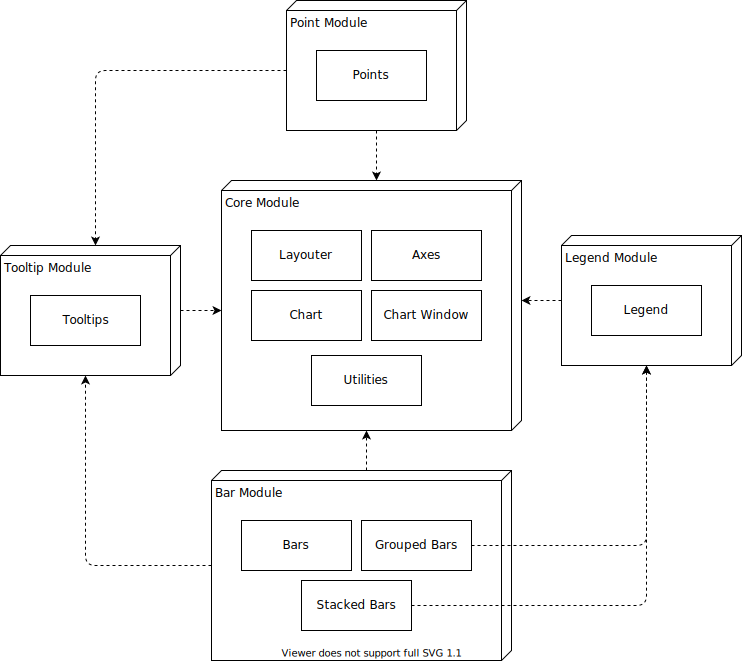
\includegraphics[keepaspectratio,width=\linewidth,height=\fullh]{diagrams/respvis-modules.pdf}
  \caption[Modules of RespVis]{
    This diagram shows the different modules of the RespVis library.
    It also shows the most important submodules contained in the individual modules.
    The directional arrows connecting modules indicate dependencies between them.
    \imgcredit{Image created by the author of this thesis using \href{https://www.diagrams.net/}{diagrams.net}.}
  }
  \label{fig:Modules}
\end{figure}


\section{Core Module}

The core module contains the necessary core functionality of the library.
It is the base module that all other modules depend on and includes various utility functions, the layouter, axes, chart base components, and chart window base components.
RespVis heavily relies on utility functions to reuse and structure recurring operations.
The core module contains utilities to deal with arrays, elements, selections, and texts, as well as geometric utilities that simplify the handling of positions, sizes, rectangles, circles, and paths.
The layouter is a custom component that enables controlling the layout of SVG elements with CSS.
% It achieves this by replicating the DOM tree of SVG elements that should be layed out with HTML \code{<div>} elements, applying the appropriate CSS configuration on the replicated elements, and storing their calculated layout information on the original SVG elements.
% Render functions can then use the stored layout information on layed out SVG elements to render their content so that it fits within the corresponding boundaries. 
Axis components have been included in the core module because they are important components that occur in nearly every visualization.
% However, since only cartesian charts have been implemented thus far, only cartesian axes can be found in the implementation.
Lastly, the chart and chart window components provide base functionalities that simplify the creation of more specialized charts and chart windows.
The core module implementation is located in the \code{src/lib/core/} directory of the project.

\subsection{Utilities}

The utilities provided by RespVis are split on multiple modules that are placed in the \code{utilities/} directory of the core module.
These modules include types and functions that perform array, element, selection and text operations as well as modules that simplify geometric operations with positions, sizes, rectangles, circles and paths.
Utility functions are grouped into modules by the type of entity they operate on.
This grouping is also reflected in the names of functions, which all begin with the type of entity a function is associated with.

\TODO{Capitalize "core module", "array utility module", ... ?}
Array utilities can be found in the \code{utilities/array.ts} module.
The \code{Array} class in the JavaScript base implementation already offers a wide variety of convenient methods to work with arrays.
These methods form a solid foundation that allows handling of a broad range of situations.
However, not everything is covered out of the box and some things require manual implementations, which is why the RespVis library offers additional functions that simplify commonly encountered tasks.
The \code{arrayEquals} function is used to verify equality of two arrays and also works if they contain nested arrays within them.
Type guard functions are used to determine the type of a variable at runtime.
For this purpose, two different array type guard functions are provided in the array utility module: \code{arrayIs}, which evaluates to true if the passed parameter is an array, and \code{arrayIs2D}, which evaluates to true if the passed parameter is a two-dimensional array.
The \code{arrayIs} function is merely a wrapper around the \code{Array.isArray} method.
Theoretically, the \code{Array.isArray} method could be used directly instead of the \code{arrayIs} function, but because the \code{arrayIs2D} function is required, the \code{arrayIs} function has also been added for consistency reasons.
The last function in the array utility module is the \code{arrayPartition} function.
This function receives an array and a partition size as parameters and returns a partitioned version of the input array with each chunk containing the number of items specified by the partition size parameter.


% elementRelativeBounds
% elementComputedStyleWithoutDefaults
% elementSVGPresentationAttrs

The element utilities module located at \code{utilities/elements.ts} in the core module contains functions and constants related to document elements.
The \code{elementRelativeBounds} function is used to calculate the bounding box of an element relative to the bounding box of its parent in viewport coordinates.
Internally, it uses the \code{getBoundingClientRect} function, which returns the actual bounding box of an element in viewport coordinates and, as opposed to other ways of accessing an element's position, it also takes transformations into account.
Every element has a set of CSS styles applied on them and the \code{Window.getComputedStyle} method can be used to access the active style of an element.
The style declaration object returned by this method contains all possible CSS properties and their values, regardless of whether or not they are set to default values.
Sometimes this behavior may be desired, but in this library, the computed style is used during the preparation of a downloadable SVG document to transform styles set in CSS to attributes on the individual elements.
If every possible style property on every element would be mapped to an attribute, the resulting SVG document would be unnecessarily bloated because only those properties that are not set to their default values actually have an effect.
For this reason, the \code{elementComputedStyleWithoutDefaults} function has been implemented to calculate the computed style of an element and remove all properties that are set to default values from the returned style declaration object.
This is implemented by adding a \code{<style-dummy>} element as a sibling of the element of interest, getting the computed styles of both elements, and calculating the difference between them.
To speed up these calculations, the \code{elementComputedStyleWithoutDefaults} function accepts an array of property names as its second parameter and will only consider the properties listed in this array.
The constant \code{elementSVGPresentationAttrs} array contains all names of the presentation attributes listed in the SVG 1.1 specification \parencite{SVG11}.
Since only these SVG attributes can be styled via CSS, only these properties need to be taken into account when preparing downloadable SVG documents.

% Transition default type variables
% Selection default type variables
% SelectionOrTransition default type variables
% Selection.attr add possible null return value
% Selection.dispatch allow Partial parameters
% isSelection
% isTransition

\TODO{When to write \code{Selection} and when to write Selection? What about plural? \code{Selections} or \code{Selection}s?}
Selection utilities are implemented in the \code{utilities/selection.ts} module.
They include typing improvements for the D3 \code{Selection}, \code{Transition}, and \code{SelectionOrTransition} interfaces and type guards to distinguish between \code{Selection}s and \code{Transition}s.
The \code{Selection}, \code{Transition}, and \code{SelectionOrTransition} interfaces allow the specification of four different type variables: the type of elements contained in the \code{Selection} or \code{Transition}, the type of data that is bound to those elements, the type of the parents of those elements, and the type of data that is bound to those parents.
In most cases, the type variables related to parent elements do not influence the logic of code using these interfaces and could be omitted to keep it more concise.
For this reason, these interface have been reexported with default types set on all of the type variables.
This means that whenever type variables need to be manually specified, only those that need to be set to specific types need to be explicitly stated.
Further typing improvements have been made to the \code{attr} and \code{dispatch} methods of the \code{Selection} interface.
The D3 type declarations of the \code{Selection.attr} method do not include \code{null} as a possible return value.
This is wrong because this method will actually result in a \code{null} value when reading an attribute that does not exist.
To fix this inconsistency and catch potential bugs related to this during compilation, the type declaration of the \code{Selection.attr} method has been overwritten in the Selection utility module to also include \code{null} as a possible return value.
A less important but nonetheless convenient improvement has been made to the type declaration of the \code{Selection.dispatch} method.
This method allows the dispatching of custom events with certain parameters that control different aspects of how this event is dispatched and the data that may be bound to it.
In practice, not all parameters need to be specified at every invocation because the implementation of the \code{Selection.dispatch} method will provide default values for all of them.
However, this is not reflected in the type declaration of the function, which requires every parameter to be provided every time the function is called.
To fix this, the Selection utility module provides a type declaration overwrite for the \code{Selection.dispatch} function that wraps the type of the parameters parameter into the \code{Partial} type.
Apart from these typing improvements, this module also provides the \code{isSelection} and \code{isTransition} type guard functions that are used to distiguish between \code{Selection}s and \code{Transition}s.


Utilities for dealing with \code{<text>} elements can be found in the \code{utilities/text.ts} module.
It contains rather basic functionalities that simply set specific data attributes to specific values on \code{<text>} elements.
The text utility module holds functions that set data attributes controlling the horizontal and vertical alignment of \code{<text>} elements, as well as their orientation.
Horizontal and vertical alignment is configured using the \code{textAlignHorizontal} and \code{textAlignVertical} functions.
These functions respectively set the \code{data-align-h} and \code{data-align-v} attribute on a Selection or Transition to the value passed into either function as a string enum parameter of type \code{HorizontalAlignment} or \code{VerticalAlignment}.
The \code{HorizontalAlignment} enum represents the string values \code{\"left\"}, \code{\"center\"} and \code{\"right\"}, while the \code{VerticalAlignment} enum represents the values \code{\"top\"}, \code{\"center\"} and \code{\"bottom\"}.
The distinct \code{data-align-h} and \code{data-align-v} attribute values are then used in the \code{respvis.css} file to declare different \code{text-anchor} and \code{dominant-baseline} values that control the alignment of \code{<text>} elements.
Text orientation is set using the \code{textOrientation} function.
This function sets the \code{data-orientation} attribute on a Selection or Transition to the value specified via the string enum parameter of type \code{Orientation}.
The \code{Orientation} enum represents the values \code{\"horizontal\"} and \code{\"vertical\"}.
These \code{data-orientation} attribute values are then used in CSS to set the \code{text-anchor}, \code{dominant-baseline}, and \code{transform} properties of a \code{<text>} element, in order to rotate it accordingly and position it correctly inside the bounding box calculated by the layouter.


% Position interface
% positionRound
% positionEquals
% positionToString
% positionFromString
% positionToAttrs (SelOrTrans)
% positionFromAttrs (SelOrTrans)
% positionToTransformAttr (SelOrTrans)

The core module also contains utilities that simplify geometric operations.
One of these utilities is the position utility module located at \code{utilities/position.ts}.
This module contains the \code{Position} interface and various functions to perform operations related to it.
The \code{Position} interface consists of the \code{x} and \code{y} number members.
Rounding these members is necessary to be able to correctly compare equality of two \code{Position}s and to not render unnecessarily long strings when transforming them into string representations.
This rounding is performed with the \code{positionRound} function, which allows the specification of the number of decimals the members variables should be rounded to.
Equality comparision between two \code{Position} variables can be performed with the \code{positionEquals} function, which evaluates to \code{true} if both \code{Position}s are equal and \code{false} if not.
To transform a \code{Position} into its string representation of the form \code{\"x, y\"}, the \code{positionToString} function can be used.
Its counterpart, the \code{positionFromString} function, can be used to transform a string in the correct format into a \code{Position}.
A large part of RespVis consists of modifying the attributes of elements.
Therefore, the \code{positionToAttrs} function can be used to set the \code{x} and \code{y} attributes of a \code{SelectionOrTransition} to the values of the \code{x} and \code{y} members of a \code{Position}.
Similarly, the \code{positionToTransformAttr} function can be used to set the \code{transform} attribute of a \code{SelectionOrTransition} to a translation representing a \code{Position}.
The position utility module also contains the \code{positionFromAttrs} function, which can be used to create a \code{Position} from the \code{x} and \code{y} attributes of a \code{SelectionOrTransition}.

% Size
% sizeRound
% sizeEquals
% sizeToString
% sizeFromString
% sizeToAttrs
% sizeFromAttrs

The size utility module is located at \code{utilities/size.ts} in the core module is very similar to the position utility module.
It contains the \code{Size} interface, which consists of the \code{width} and \code{height} number member variables.
The \code{sizeRound} function is used to round the member variables of a \code{Size} object to a certain number of decimals.
To compare two \code{Size} objects for equality, the \code{sizeEquals} function can be used.
Similar to the equivalent functions in the position utility module, the \code{sizeToString} and \code{sizeFromString} functions can be used to convert between \code{Size} objects and their string representations.
Moreover, the \code{sizeToAttrs} can be used to set the \code{width} and \code{height} attributes of a \code{SelectionOrTransition} to the values of a \code{Position} object and the \code{sizeFromAttrs} function can be used to create a new \code{Position} object from the values of these attributes.

% Rect
% rectRound
% rectEquals
% rectToString
% rectFromString
% rectToAttrs
% rectMinimized
% rectFitStroke
% rectPosition
% rectCenter
% rectLeft, rectRight, rectTop, rectBottom
% rectTopLeft, rectTopRight, rightBottomRight, rightBottomLeft

Utilities for dealing with rectangles can be found in the rectangle utility module, which is located under \code{utilities/rect.ts} in the core module.
This module contains the \code{Rect} interface, which is the union of the \code{Position} and \code{Size} interfaces and therefore describes an object with the number member variables \code{x}, \code{y}, \code{width}, and \code{height}.
Similar to the position and size utility modules, this module contains the \code{rectRound} function to round \code{Rect} objects, the \code{rectEquals} function to compare two of them for equality, the \code{rectToString} and \code{rectFromString} functions to convert between \code{Rect} objects and their string representations, and the \code{rectToAttrs} and \code{rectFromAttrs} functions to convert between objects and \code{x}, \code{y}, \code{width}, and \code{height} attributes.
Since the \code{Rect} interface is a combination of the \code{Position} and \code{Size} interfaces, most of the functions in this module internally use the functions provided by the position and size utility modules.
The \code{rectMinimized} function is used in transitions that grow or shrink a \code{<rect>} element from or to their center.
It creates a minimized version of the passed \code{Rect}, which is infinitely small and positioned at the original \code{Rect}'s center.
When declaring a stroke for SVG elements, it is drawn exactly on the outline of an element's silhouette.
This means that a stroke will extend outside the original bounds of an element by half the stroke width, which can lead to unwanted artefacts like the stroke of bars in a bar chart overlapping over the chart's axes.
To counteract this, the \code{rectFitStroke} function is provided to adjust the bounding box of \code{Rect} objects to account for a stroke of a certain width around them.
Lastly, the rectangle utility module provides functions to calculate specific positions inside of rectangles.
The most generic of these functions is the \code{rectPosition} functions.
This function enables the calculation of a position inside of a rectangle via a two-dimensional parameter that expresses a position as the percental width and height distance from a rectangle's top-left corner.
All other position-calculating rectangle utility functions are simply shorthand functions that internally call the \code{rectPosition} function.
The \code{rectCenter} function returns a \code{Position} object representing the center position of a \code{Rect} object.
The \code{rectLeft}, \code{rectRight}, \code{rectTop}, and \code{rectBottom} functions return \code{Position} objects that represent the middle position of a \code{Rect} object's edges.
Similarly, The \code{rectTopLeft}, \code{rectTopRight}, \code{rectBottomRight}, \code{rectBottomLeft} functions can be used to calculate the corner positions of a rectangle.

% Circle
% circleRound
% circleEquals
% circleToString
% circleFromString
% circleToAttrs
% circleFromAttrs
% circleMinimized
% circleFitStroke
% circlePosition
% circleInsideRect
% circleOutsideRect

The last geometric primitive whose handling is simplified by a RespVis utility module is a circle.
The circle utility module can be found at \code{utilities/circle.ts} in the core module.
It contains the \code{Circle} interface, which describes a circle object as a \code{center} property of type \code{Position} and a \code{radius} property of type \code{number}.
This module also contains equivalent functions to those found in previously mentioned utility modules: \code{circleRound}, \code{circleEquals}, \code{circleToString}, \code{circleFromString}, \code{circleToAttrs}, \code{circleFromAttrs}, \code{circleMinimized}, and \code{circleFitStroke}.
Furthermore, the \code{circlePosition} function can be used to calculate positions using an angle that defines the direction and an optional parameter that defines the distance from the circle's center as a percentage of the circle's radius.
The circle utility module also contains functions to create circles from rectangles.
These functions are the \code{circleInsideRect} function to calculate the largest circle that can fit inside of a rectangle and the \code{circleOutsideRect} function to calculate the smallest circle that encloses a rectangle.

% pathRect
% pathCircle

The purpose of the path utility module is to provide functions that simplify the creation of path definitions that can be set on \code{<path>} elements.
It is located at \code{utilities/path.ts} in the core module and only contains a small number of functions.
The \code{pathRect} function creates a path definition that represents a rectangle. 
A \code{<path>} element with a path definition representing a rectangle can be used instead of a \code{<rect>} element. 
Similarly, the \code{pathCircle} function creates a path definition that represents a circle.
Such a path definition is used on a \code{<path>} element to render a circle instead of using a \code{<circle>} element.
The reason for using \code{<path>} elements rather than more descriptive shape elements is that path elements can change their shape dynamically without replacing elements.
Since only the \code{d} attribute of a path needs to change when the path's shape is altered, it is also possible to smoothly transition between shapes by interpolating the path definition strings.

\subsection{Layouter}
\label{sec:Layouter}

The Layouter is the most novel contribution of this work.
It is a component that is wrapped around an SVG document and allows to configure the layout of elements in this document with CSS.
Instead of implementing a custom layout algorithm, the Layouter builds on layout engines integrated in browsers, which have already been summarized in Section~\ref{sec:BrowserEngines}.
Earlier proof of concept implementations used the FaberJS \parencite{FaberJS} and Yoga \parencite{Yoga} layout engines to calculate layouts, but these implementations were not further pursued because they limited layouting to either Grid or Flexbox-based constraints.
Furthermore, the use of already existing browser functionality in the current implementation leads to a reduced bundle size and to visualization authors being able to use all the layouting capabilities natively offered by browsers.

CSS has always been the foundation of responsive web design for HTML-based websites because of its ability to adapt the presentation of elements and the possibility of defining different presentations for different contexts via media queries.
A large part of the responsive power that CSS offers comes from its ability to change the positioning and layout of elements.
As already mentioned in previous chapters, CSS can be used to style certain aspects of SVG documents, but it is not possible to use CSS layouting techniques to position SVG elements.
Even though there are already other visualization libraries such as Chartist \parencite{Chartist} and Highcharts \parencite{Highcharts} that allow the use of CSS to style visualizations, none of them offer the possibility to modify the layout of visualizations via CSS.
This means that visualization authors have to learn and use custom APIs to position elements, which limits the range of possible layouts to those supported by the individual libraries. 

The Layouter distinguishes between laid-out and non-laid-out elements because not every element in a visualization profits from being laid out by it. 
Laid-out elements are elements whose position and size are being calculated by the Layouter, whereas non-laid-out elements are ignored during the layout process. 
Theoretically, the layouter could be used to position all elements of a visualization since it is only necessary to determine a good mapping that maps a rectangular bounding box to the desired SVG shape for each element.
However, the positioning of elements in a visualization is constrained more strictly than the positioning of elements in typical HTML documents.
The content of a visualization is communicated more through visual features such as position, size, and shape of elements rather than simply through text which can be positioned much more freely.  
For this reason, many elements of a visualization must be positioned at specific locations with specific dimensions, which means there is very little profit in laying them out with an elaborate layout algorithm.
These exactly-positioned elements like the \code{<rect>} elements of bar series and the \code{<circle>} elements of point series are usually positioned directly via their SVG attributes.
Positioning them via the Layouter would be rather pointless and only cause unnecessary overhead.

The layout process can be seen in Figure~\ref{fig:LayoutProcess} and consists of three phases that have been implemented in the \code{layouterCompute} function:
\begin{enumerate}
\item Replication:
The structure of the SVG document that shall be laid out must be replicated with HTML \code{<div>} elements. These elements are referred to as \enquote{layout elements} and they have the same classes and \code{data-*} attributes as the original SVG elements they are replicating.
This replication of the SVG document with HTML documents is necessary because CSS-based positioning can only affect HTML elements.

\item Layout:
The replicated layout elements are affected by CSS rules that configure their positioning and are automatically laid out by browsers. 
If the Selectors of CSS rules used to style SVG elements only select them using classes and \code{data-*} attributes, the layout of these elements can be directly configured in these rules because they will also be applied to the corresponding layout elements.

\item Synchronization:
The positions of the layout elements are synchronized with their respective SVG elements.
This means that the calculated bounding boxes of layout elements are set as \code{bounds} attributes on SVG elements, which can be used in subsequent renderings.
In addition to that, the Layouter sets different default attributes on different types of SVG elements that aim to represent the boundaries of individual elements.
\end{enumerate}

\begin{figure}[tp]
\centering

\includegraphics[keepaspectratio,width=\linewidth,height=\fullh]{diagrams/respvis-layout-process.pdf}
\caption[Layout Process of the Layouter]{
  This diagram shows the three phases of the layout process of the RespVis Layouter. 
  During the replication phase, the SVG document that shall be laid out is replicated with HTML \code{<div>} elements. 
  Afterward, these HTML elements are laid out by the browser in the layout phase, and the positions of the laid-out HTML elements are applied to their respective SVG elements during the synchronization phase.
  \imgcredit{Image created by the author of this thesis using \href{https://www.diagrams.net/}{diagrams.net}.}
}
\label{fig:LayoutProcess}
\end{figure}


During the replication process, the structure of an SVG document is replicated with HTML \code{<div>} elements. 
This replication was implemented using a hierarchical D3 data join in which the original SVG elements are bound as data objects to layout elements.
This hierarchical data join results in a counterpart in the hierarchy of layout elements for each SVG element that should be affected by the layouter.
Since not every SVG element should be positioned via the Layouter, the Layouter must know which to ignore.
For this, the \code{data-ignore-layout} and \code{data-ignore-layout-children} attributes have been introduced.
Elements that have the \code{data-ignore-layout} attribute or are children of elements that have the \code{data-ignore-layout-children} attribute will not be replicated.

To configure the layout of layout elements in CSS, it must be possible to select them uniquely with a CSS Selector.
This Selector should be as similar as possible to the Selector of the original SVG element to make it as easy as possible to configure the CSS properties of layout elements.
For this purpose, the class attributes and all data-* attributes of SVG elements are copied to their corresponding layout elements.
In addition to the classes of the replicated SVG element, the layout class is set on all layout elements.
By doing this, it is possible to specifically select the layout element of an SVG element via the same Selector by adding the layout class to the same Selector. 
If CSS rules of SVG elements use only classes and data attributes in their Selectors, the properties of corresponding layout elements can directly be configured in the same rules.
An example of how the replicated layout element tree of an SVG document looks can be seen in Listing~\ref{list:LayouterStructure}.
Furthermore, an example of CSS rules that set various properties of SVG elements and their layout elements can be seen in Listing~\ref{list:LayouterCSS}.  

\begin{samepage}
\lstinputlisting[%
  float=tp,
  aboveskip=\floatsep,
  belowskip=\floatsep,
  xleftmargin=0cm,              % no extra margins for floats
  xrightmargin=0cm,             % no extra margins for floats
  %
  basicstyle=\footnotesize\ttfamily,
  frame=shadowbox,
  numbers=left,
  label=list:LayouterStructure,
  caption={[Replicated Layout Structure of an SVG Document]%
    The replicated layout element structure of an SVG document.
    Every SVG element has a corresponding layout element that has the same classes and \code{data-*} attributes.
    In addition to the classes of the original SVG element, every layout element also has the \code{layout} class to allow specific targeting of layout elements via CSS Selectors.
  },
]{listings/layouter-structure.html}
\end{samepage}

\begin{samepage}
\lstinputlisting[%
  float=tp,
  aboveskip=\floatsep,
  belowskip=\floatsep,
  xleftmargin=0cm,              % no extra margins for floats
  xrightmargin=0cm,             % no extra margins for floats
  %
  basicstyle=\footnotesize\ttfamily,
  frame=shadowbox,
  numbers=left,
  label=list:LayouterCSS,
  caption={[CSS Rules to Style SVG]%
    These CSS rules are used to configure the layout and style of an SVG document that is being laid out by the Layouter.
    Since the Selectors of these CSS rules only use \code{class} and \code{data-*} attributes to match elements, the same rule can be used to configure the properties of an SVG element and its corresponding layout element.  
    The structure of the SVG document and its replicated layout elements can be seen in Listing~\ref{list:LayouterStructure}.
  },
]{listings/layouter-css.css}
\end{samepage}

The size of dynamically-sized elements depends on the size of their content.
Since layout elements exist separately from their SVG elements and can not access their content, a manual solution had to be implemented that sets the size of layout elements to the content size of their SVG elements when required.
An example of dynamically-sized elements is \code{<text>} elements because their size is rarely declared in absolute units and usually depends on the size of their text contents. 
The custom \code{--fit-width} and \code{--fit-height} CSS properties were introduced to activate the manual copying of dimensions from SVG elements to their layout elements. 
These boolean properties can be set in CSS rules and are being checked during the replication phase via the \code{window.getComputedStyle} method.
If at least one of these properties is set to true, the dimensions of the SVG element are calculated with the \code{Element.getBoundingClientRect} method and respectively set as \code{width} or \code{height} properties of the \code{style} attribute on the corresponding layout element.
By doing this, layout elements will have the same size as their svg elements and can be properly used in the calculation of the overall layout. 

Layout elements are automatically laid out by the browser during the layout phase of the layout process. 
Since the layout elements are simply \code{<div>} elements that have been styled in CSS rules, the browser can position them automatically via its integrated layout engine.
This positioning happens as soon as the layout elements have been rendered.
After this, the final bounding boxes of layout elements can be calculated and used for further operations.  

In the synchronization phase of the layout process, the Layouter iterates over all the layout elements, calculates their bounding boxes, and set this boundary information as attributes on the corresponding SVG elements.
Bounding boxes of layout elements are calculated relative to their parent elements using the \code{elementRelativeBounds} utility function.
This bounding box is then converted to its string representation via the \code{rectToString} utility function and set as the \code{bounds} attribute on the corresponding SVG elements. \TODO{Rename bounds attr to data-bounds}
The \code{bounds} attribute can then be deserialized to a \code{Rect} object whenever the bounding box of an SVG element is needed in subsequent renderings of SVG components. 
In addition to setting the \code{bounds} attribute of SVG elements, the Layouter also sets specific attributes on different types of SVG elements that make them fit into their calculated bounding boxes.
These attributes can, of course, be overwritten in later renderings, but they represent sensible defaults that express the boundaries of laid-out elements.
If the Layouter would not set these default attributes, they would have to be set manually on every laid-out element during the rendering process, which would be less convenient and lead to duplicated code in various places.
For SVG elements that can be mapped directly to rectangular areas, such as \code{<svg>} and \code{<rect>} elements, the Layouter sets the \code{x}, \code{y}, \code{width}, and \code{height} attributes to the values of their bounding boxes.
SVG shape elements that have explicit sizes and positions but are not rectangular, such as \code{<circle>} and \code{<line>} elements, also receive attributes that make them fit into their boundaries. 
Other SVG elements that are not explicitly sized, such as \code{<g>} and \code{<text>} elements, are merely moved to the correct position by setting their \code{transform} attribute to a translation so that their top-left corners aligns with the top-left corners of their bounding boxes. 
The Layouter does not automatically recalculate the dimensions of exactly-positioned elements based on the changed dimensions of the composite \code{<svg>} or \code{<g>} element containing them.
This has to be manually implemented in the render functions of the various components.

Using the Layouter requires a more complex rendering process than would be needed if the boundaries of elements would already be known before rendering them.
The way the Layouter works, some elements need to be rendered before calculating the layout, and afterward, when the positions and sizes of all elements are known, the visualization needs to be rendered in its final form. 
This visualization rendering process when using the Layouter consists of three phases and is shown in Figure~\ref{fig:RenderProcess}.
The three phases of the render process are the first rendering phase to render elements affecting the layout, the layouting phase, and the second rendering phase to render elements affected by the layout.
In the first rendering phase, all elements and attributes that affect the layout of a visualization need to be rendered.
This mostly includes laid-out container \code{<svg>} and \code{<g>} elements that contain exactly-positioned child elements, but it also means that the contents of dynamically-sized elements, such as \code{<text>} elements and axes, need to be fully rendered in this phase too.
The layouting phase is where all the operations of the already-described layout process are being performed.
During this phase, the bounding boxes of laid-out elements are calculated and persisted as attributes that can be accessed during the second rendering phase.
In the second rendering phase, the desired bounding box position and size of every element is known and can be used to perform a second rendering of the complete visualization.
Here, every element affected by the layout, which is every element, is rendered at its final position with its final dimensions.
In theory, the first and second rendering phases of components could be implemented in separate functions.
However, it is more convenient to invoke the same render function twice and perform some operations only if the appropriate \code{bounds} attribute has already been set.


\begin{figure}[tp]
\centering
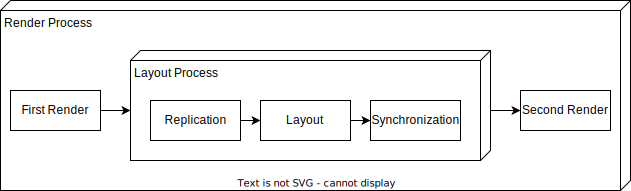
\includegraphics[keepaspectratio,width=\linewidth,height=\fullh]{diagrams/respvis-render-process.pdf}
\caption[Render Process When Using the Layouter]{
  This diagram shows the three phases of the render process when using the RespVis Layouter. 
  During the first render phase, every element that affects the layout needs to be rendered.
  The layout phase of the render process is equivalent to the layout process described in Figure~\ref{fig:LayoutProcess}.
  In this phase, the Layouter calculates the final positions and sizes of laid-out elements and stores them as attributes on the SVG elements.
  During the second render phase, all elements of the visualization are rendered at their final positions with their final dimensions by using the boundary information calculated in the layout phase.
  \imgcredit{Image created by the author of this thesis using \href{https://www.diagrams.net/}{diagrams.net}.}
}
\label{fig:RenderProcess}
\end{figure}


\subsection{Axes}

% axisData
%   scale
%   title
%     orientation
%   subtitle
%     orientation
%   configureAxis
%     d3 axis
%   default values
% axisRender
%   structure
%     .title (dynamically sized wh)
%     .subtitle (dynamically sized wh)
%     .ticks-transform (dynamically sized w or h) warum?
%       .ticks
%     laid out with CSS Grid
%   d3 axis function to render ticks
%     delete attributes and use data attributes and css to configure presentation of axis
% axisBottomRender
%   .axis-bottom
%   CSS grid with 3 rows and 1 full width column
%   title and subtitle orientations
%   tick text alignment
% axisLeftRender
%   .axis-left
%   CSS grid with 3 columns and 1 full height row
%   title and subtitle orientations
%   tick text alignment


Axes are used to visualize scales representing the mapping of abstract values to two-dimensional positions.
The implementation of all available axis components can be found in the \code{axis.ts} file in the core module.
Currently only cartesian axes are provided by the RespVis library since so far only cartesian charts have been implemented.
These cartesian axis components are distinguished by their position relative to the draw area of a visualization and at the time of writing only left and bottom axis components have been implemented in the RespVis library.
These are by far the most commonly encountered positions of cartesian axes and have been chosen because they cover most use cases. 
An axis consists of ticks, which are the actual visualization of a scale, and an optional title and subtitle, which can be rendered to additionally describe the configuration of the visualized scale. 
An example of what a rendered left and bottom axis might look like can be seen in Figure~\ref{fig:Axes}. 

\begin{figure}[tp]
\centering
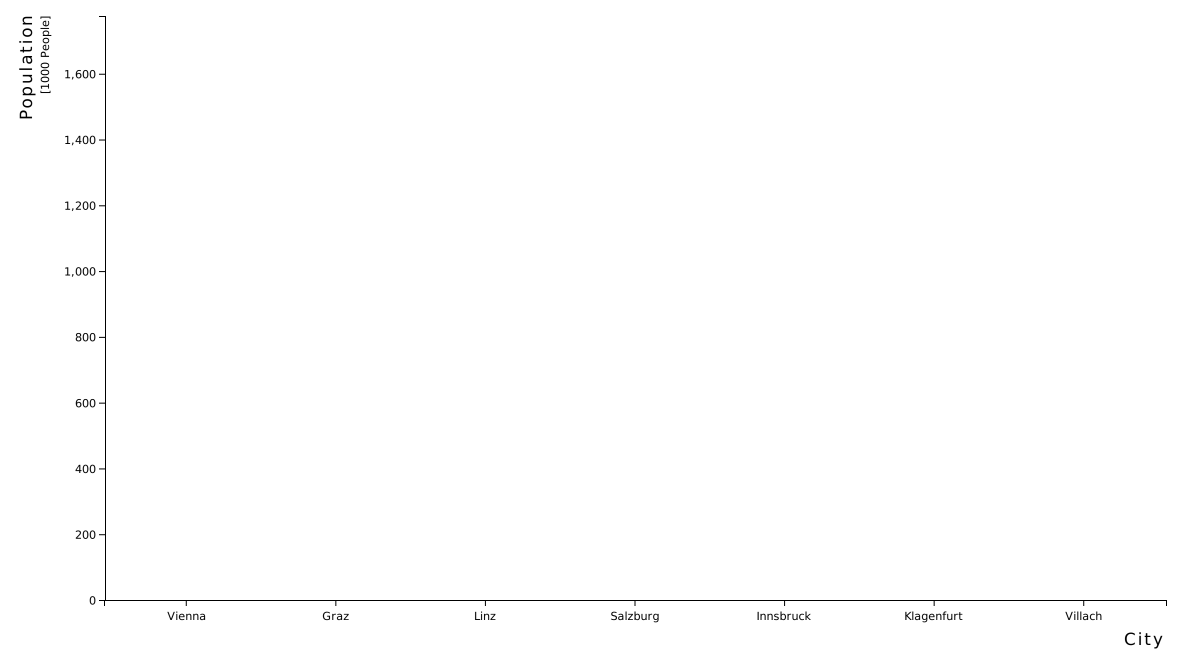
\includegraphics[keepaspectratio,width=\linewidth,height=\fullh]{diagrams/axes.pdf}
\caption[RespVis Axis Components]{
  This figure shows how a rendered left and bottom axis may look like.
  The left axis consists of a title, subtitle, and ticks, whereas the bottom axis only consists of ticks and a title. 
  \imgcredit{Image created by the author of this thesis using RespVis and \href{https://inkscape.org/}{Inkscape}.}
}
\label{fig:Axes}
\end{figure}
  

The \code{Axis} interface describes the shape of a data object with which the rendering of an axis can be configured.
It includes a \code{scale} property, which represents the scale that has to be visualized, the \code{title} and \code{subtitle} string properties, and the \code{configureAxis} function property, which can be used to configure the underlying D3 axis before rendering it.  
Like most other components, axis components consist of two main functions: a data creation function and a render function.
The \code{axisData} function is used to create a data object in the form of the \code{Axis} interface.
It is called with a \code{Partial<Axis>} object as parameter and returns a new object with all non-set but required properties of the parameter object filled with default values.
The \code{axisBottomRender} and \code{axisLeftRender} functions are used to render a left and bottom axis in a composite element on which an axis has been configured using a bound \code{Axis} data object. 
These two render functions use the non-exported \code{axisRender} base function to avoid duplicate code.
All axes have the same structure of elements which are positioned and styled as much as possible using CSS.
The root of an axis is a CSS Grid container and defines the layout of the title, subtitle and ticks elements.
The default configuration of a left axis positions these elements in a three-column layout in which the title, subtitle and ticks elements are placed in this order from left to right.
For a bottom axis, the default configuration positions the same elements in a three-row layout in which the ticks, title and subtitle elements are placed in this order from top to bottom.
Furthermore, the title and subtitle elements of a left axis are vertically oriented to save horizontal space using the \code{textOrientation} utility function.
The RespVis axis components internally use the \code{axisBottom} and \code{axisLeft} functions from the D3 axis module \parencite{D3Axis} to render the ticks of an axis.
Since these D3 functions use attributes to position and style the individual elements of the ticks of an axis, as many of these attributes as possible must be removed directly after the ticks have been rendered to allow configuration via CSS. 

\subsection{Chart}

% higher-level components that render lower-level components such as axes, legends, and series. 
% chart
%   chartRender
%     default attributes of every chart
%     .chart
%     xmlns
% chart cartesian
%   ChartCartesian
%     xAxis, Axis, data object
%     yAxis, Axis, data object
%     flipped, boolean, flipping of x and y axes
%   chartCartesianData
%     input
%       Partial<ChartCartesian> with Partial<Axis> as xAxis and yAxis type
%     default values
%   chartCartesianRender
%     chart
%     .chart-cartesian
%       .draw-area
%         .background, invisible, for capturing events
%   chartCartesianAxesRender
%      left axis with either xAxis or yAxis data depending on value of flipped
%      bottom axis with either xAxis or yAxis data depending on value of flipped
%      .x-axis
%      .y-axis
%   contents laid out with CSS grid
%     left axis, bottom axis, draw area, potential legend
%     dynamic draw-area size to fill available space

\TODO{Capitalize "Chart Component" or "Chart component"? How about only "chart" without "component"? Capitalize "Chart" everytime it's used?}
charts sind higher-level components die eine vollstaendige visualisierung inklusive achsen, legenden und series representieren.
ein beispiel eines gerenderten RespVis charts der zwei achsen, eine grouped bar series, eine label series und eine legend beinhaltet kann in Figure~\ref{fig:Chart} gesehen werden.
Ein chart wird typischerweise in dem root \code{<svg>} element eines SVG dokumentes gerendert welches zumindest die \code{chart} klasse im \code{class} attribute und den angemessenen SVG namespace im \code{xmlns} attribute gesetzt hat.
Diese attribute koennen in spezifischeren chart komponenten entweder manuel oder ueber die \code{chartRender} funktion aus der \code{chart.ts} datei im core module, welche nur diese attribute setzt, gesetzt werden.

\begin{figure}[tp]
  \centering
  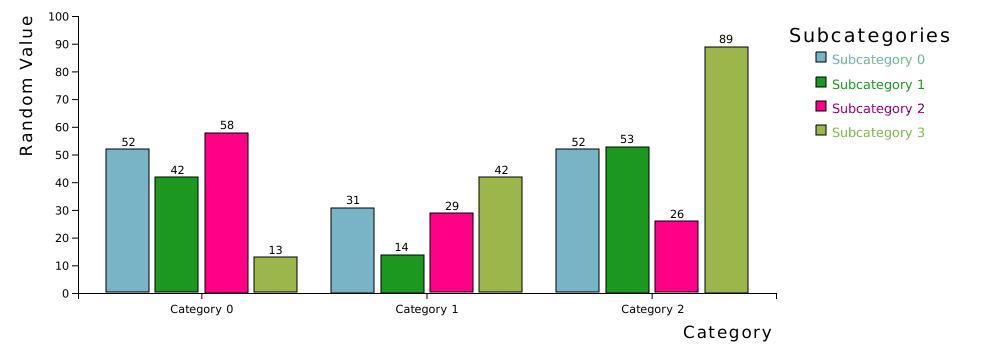
\includegraphics[keepaspectratio,width=\linewidth,height=\fullh]{diagrams/chart.pdf}
  \caption[Chart Example]{
    An example of a chart that contains two axes, a grouped bar series, a label series and a legend.
    This chart has been rendered with the RespVis library.
    \imgcredit{Image created by the author of this thesis.}
  }
  \label{fig:Chart}
\end{figure}

wie bereits erwaehnt beinhaltet die RespVis library aktuell nur die implementationen von kartesischen charts welche daten in einem kartesischen koordinatensystems visualisieren.
die implementierung der basis funktionen von kartesischen charts befindet sich in der \code{chart-cartesian.ts} datei im core module. 
das \code{ChartCartesian} interface beschreibt ein data object fuer die konfiguration von kartesischen charts.
diese data objects beinhalten die \code{xAxis} und \code{yAxis} \code{Axis} properties mit welchen jeweils die X und Y achsen des charts beschrieben werden.
das transponieren von achsen ist ein nuetzliches pattern um die responsiveness von visualisierungen zu verbessern und wird mittels des \code{flipped} boolean properties konfiguriert.
wenn das \code{flipped} property auf \code{false} gesetzt ist, wird das \code{xAxis} object fuer die konfiguration der bottom axis und das \code{yAxis} object fuer die konfiguration der left axis verwendet. 
wenn es auf \code{true} gesetzt ist, ist es genau umgekehrt.

die \code{chartCartesianData} funktion wird verwendet um ein data object in der form des \code{ChartCartesian} interface zu erzeugen.
diese funktion erhaelt ein partielles data object bei welchem nur jene properties gesetzt sind welche fuer den aufrufenden code von interesse sind.
alle nicht gesetzten properties werden mit standardwerten befuellt.
die standardwerte der \code{xAxis} und \code{yAxis} properties werden ueber die \code{axisData} funktion aus dem axis submodule gesetzt.
das \code{flipped} property wird, falls es nicht ueber den input parameter spezifiziert wird, auf \code{false} gesetzt.

das rendern von kartesischen charts ist auf zwei funktionen aufgeteilt die seperat voneinander aufgerufen werden muessen.
diese aufteilung wurde gemacht weil nicht alle teile eines kartesischen charts zum selben zeitpunkt gerendert werden koennen.
die generelle struktur eines charts muss gerendert werden bevor irgendetwas anderes gerendert werden kann da dies das draw area container element beinhaltet in welches individuelle series componenten gerendert werden muessen.
die achsen eines charts benoetigen eine vollstaendig initialisierte scale um korrekt gerendert werden zu koennen.
die range einer scale, also der wertebereich in welchen abstrakte werte gemappt werden, haengt allerdings von den dimensionen der draw area boundary ab und wird erst waehrend der render funktion der individuellen series components, welche in die draw area gerendert werden, initialisiert.    
aus diesem grund duerfen achsen erst nach allen series components gerendert werden um eine vollstaendig initialisierte scale zu gewaehrleisten.

die struktur eines kartesischen charts wird mit der \code{chartCartesianRender} funktion gerendert.
diese fuktion setzt die notwendigen chart attribute und die \code{chart} klasse mit der \code{chartRender} funktion.
Weiters wird mit dieser funktion die \code{chart-cartesian} klasse auf den root elementen der Selection gesetzt mit welcher die funktion aufgerufen wurde.
die \code{chartCartesianRender} funktion fuegt fuegt ausserdem noch ein \code{<svg>} element mit der \code{draw-area} klasse als child element des component root elementes ein.
die draw area ist das container element in welches die individuellen series components eines charts gerendert werden.
standardmaessig wird das \code{overflow} CSS property der draw area auf \code{visible} gesetzt um eventuell ueberlappende elemente nicht zu clippen.
ein \code{<svg>} element ohne tatsaechlichen content ist nicht in der lage input events abzufangen.
das bedeutet dass es zum beispiel nicht moeglich waere mittels scroll events eine zoom interaktion zu steuern wenn der cursor sich ueber der leeren flaeche der draw area befindet.
um dem entgegenzuwirken erzeugt die \code{chartCartesianRender} funktion fuer jede draw area ein transparentes \code{<rect>} background element welches die gesamte flaeche der draw area fuellt und welches es ermoeglicht input events auch in bereichen zu generieren in welchen sich keine series elemente befinden.

die \code{chartCartesianAxesRender} funktion wird verwendet um die achsen eines kartesischen charts zu rendern.
diese funktion darf nur auf elementen mit einem gebundenen \code{ChartCartesian} data object und nach der vollstaendigen initialisierung der scales, welche mit den achsen visualisiert werden sollen, aufgerufen werden.
meist bedeutet dies fuer die reihenfolge an operationen einer spezifischerer kartesischen chart component, dass zu beginn die struktur des charts mittels der \code{chartCartesianRender} funktion erzeugt werden muss, gefolgt von dem rendern der gewuenschten series components, und erst danach duerfen die achsen mittels der \code{chartCartesianAxesRender} funktion gerendert werden.
die \code{chartCartesianAxesRender} function erzeugt zwei \code{<g>} elemente und rendert eine left und eine bottom axis auf ihnen.
je nachdem ob das \code{flipped} property im gebundenen data object auf \code{true} oder \code{false} gesetzt ist, wird das \code{xAxis} data object fuer die konfiguration der bottom oder left axis verwendet und das \code{yAxis} data object jeweils fuer die andere achse.
nachdem die achsen gerendert wurden wird auf der achse auf welcher das \code{xAxis} data object gebunden ist die \code{x-axis} klasse und auf der anderen achse die \code{y-axis} klasse gesetzt. 
diese klassen werden gesetzt um die auswahl der konkreten achsen welche die jeweilige konfiguration representieren ueber CSS Selectors zu ermoeglichen.

wie es in der RespVis library ueblich ist, wird alles moegliche an positionierung und styling ueber CSS konfiguriert.
die elemente eines kartesischen charts werden ueber ein CSS Grid layout positioniert.
standardmaessig wird ein grid erzeugt welcher die \code{axis-left}, \code{axis-bottom}, \code{draw-area}, und \code{legend} areas definiert.
die groesse der meisten zeilen und spalten dieses grids ist auf \code{auto} gesetzt, was bedeutet dass deren groesse von der groesse ihres inhaltes abhaengt. 
die ausnahme hiervon sind die zeile und spalte in welchen sich die draw area befindet.
deren groesse ist auf \code{1fr} gesetzt um zu erreichen dass die draw area den gesamten restlichen horizontalen und vertikalen platz einnimmt der nicht von den anderen zeilen und spalten eingenommen wird.
die standardkonfiguration der \code{chart-cartesian} klasse sieht eine positionierung einer eventuellen legende rechts von der draw area vor.
um die position der legende zu veraendern kann entweder direkt der grid ueber CSS angepasst werden oder eine der vorkonfigurierten positionen kann ueber das \code{data-legend-position} attribut aktiviert werden.
um das setzten des \code{data-legend-position} attributes zu vereinfachen kann die \code{chartLegendPosition} funktion, welche dieses attribut auf den wert eines mitgegebenen \code{LegendPosition} enum parameters setzt, verwendet werden.


\subsection{Chart Window}

% wrappers around charts that handle the render process and add a toolbar to configure charts and perform various operations.
% chartWindowRender
%   div.chart-window
%     div.toolbar, toolbarRender
%       div.menu-tools, menuToolsRender
%         menuDropdownRender
%         no chevron
%         text unicode burger menu, trigram for heaven, https://graphemica.com/%E2%98%B0, U+2630
%     div.layouter
%   resizeEventListener
% menuDropdownRender
%   .menu
%     span.chevron, unicode, left pointing,
%     span.text
%     ul.items
%       positioning and styling via CSS
%       showing via CSS
%       highlighting via CSS

% toolFilterNominal
%   one of the tools provided by the library is the nominal filtering tool that can be used to filter a nominal dimension of the rendered data.
%   nominal data is simply labeled data where no quantitative value is assigned to the individual values.  
%   text, options, keys
%   menuDropdownRender
%   .item, seriesCheckboxRender
%     container, labels, keys
%     containerElement.checkbox
%       input[type=checkbox][id=uuid()]
%       label[for=input.id]
% tool download svg
%   dont describe in too much detail as it will be included in selected topics chapter
% resize event dispatcher

\TODO{Capitalize "Chart Window"?}
chart windows sind wrapper komponenten um charts die einen chart innerhalb eines Layouter container elementes rendern und mit einer toolbar dekorieren.
ein beispiel eines chart windows mit einem ausgeklappten tool menue in welchem sich zwei nominale filtering tools und ein svg download tool befinden kann in Figure~\ref{fig:ChartWindow} gesehen werden.
die implementierung der chart window komponente befindet sich in der \code{chart-window.ts} datei im core module.
diese komponenten stellen einen noch higher-level layer als charts dar und werden verwendet um den render prozess und die konfiguration von charts zu managen.
in den meisten anderen visualization libraries werden charts als der hoechste level an komponenten die konfiguriert werden koennen zur verfuegung gestellt.
typischerweise bedeutet das, dass zusaetzliche HTML elemente fuer die runtime configuration von charts von der einbettenden webseite selbst erzeugt und gemanaged werden muessen.     
ein chart window wird ausserhalb des SVG dokumentes eines charts auf einem HTML \code{<div>} element mit der \code{chartWindowRender} funktion gerendert.
ihre struktur besteht aus einem \code{<div>} element in welches die toolbar mit der \code{toolbarRender} funktion gerendert wird und aus einem weiteren \code{<div>} element auf welchem ein Layouter mit der \code{layouterRender} funktion initialisiert wird. 
das SVG dokument eines charts wird dann an das \code{<div>} element des Layouters als child angehaengt.

\begin{figure}[tp]
  \centering
  \includegraphics[keepaspectratio,width=\linewidth,height=\fullh]{images/chart-window.png}
  \caption[Chart Window Example]{
    An example of a chart that is wrapped in a chart window.
    The tool menue has been expanded by hovering over it and the menu entries of two nominal filtering tools and the download SVG tool can be seen inside.
    \imgcredit{Image created by the author of this thesis.}
  }
  \label{fig:ChartWindow}
\end{figure}


zum aktuellen zeitpunkt befindet sich in der toolbar nur das tool menu als einziges element.
das tool menu ist ein dropdown menue in welchem die einzelnen tools als menueeintraege oder als untermenues zu finden sind.
ein dropdown menu wird ueber die \code{menuDropdownRender} funktion auf den elementen der mitgegebenen Selection gerendert.
diese funktion setzt die \code{menu} klasse auf den root elementen auf welchen das dropdown menue gerendert wird.
ein dropdown menue besteht aus einem \code{<span>} element mit der \code{chevron} klasse dessen text content ein nach links zeigendes Unicode chevron symbol ist, einem zweiten \code{<span>} element mit der \code{text} klasse dessen text der titel des dropdown menues ist, und einem \code{<ul>} element mit der \code{items} klasse dass die unterelemente des dropdown menues beinhaltet.
die unterelemente eines dropdown menues werden ueber CSS absolut positioniert und angezeigt sowie highlighted solange eine hover interaktion auf dem menue stattfindet.
das tool menue wird ueber die \code{menuToolsRender} funktion erzeugt welche intern die \code{menuDropdownRender} funktion verwendet um das tool menue als dropdown menue zu initialisieren.
das root dropdown menue des tool menues wird ohne chevron symbol gerendert und enhaelt ein Unicode symbol in seinem \code{<span>} element mit der \code{text} klasse. 
das symbol dass fuer das tool menue verwendet wurde ist das \enquote{trigram for heaven} Unicode symbol mit dem code U+2630 welches haeufig fuer burger menues verwendet wird.

\TODO{Rename nominal filtering tool to categorical filtering tool}
% Categorical variables are those that have discrete categories or levels. Categorical variables can be further defined as nominal, dichotomous, or ordinal. Nominal variables describe categories that do not have a specific order to them. These include ethnicity or gender.
das core module stellt tools zur verfuegung die zu den tool menues von spezifischeren chart windows hizugefuegt werden koennen.
eines dieser tools ist das nominale filtering tool welches sich in der \code{tools/tool-filter-nominal.ts} datei im core module befindet.
dieses tool wird verwendet um eine nominale datendimension eines visualsierten datasets ueber ein dropdown menue dass eine checkbox series beinhaltet zu filtern.
nominale daten sind im gegensatz zu ordinalen daten nur gelabelte oder kategorische daten deren werten kein quantitativer wert zugewiesen ist und welche daher keine reihenfolge besitzen und auch nicht sortiert werden koennen.
das data object fuer die konfiguration eines nominalen filter tools wird durch das \code{ToolFilterNominal} interface beschrieben.
dieses interface enthaelt ein \code{text} string property welches den titel des dropdown menues definiert, ein \code{options} string array property welches die einzelnen optionen die gefiltert werden koennen definiert, und ein \code{keys} string array property welches die keys der einzelnen optionen definiert. 
die \code{toolFilterNominalData} funktion wird verwendet um ein data objekt vom typ \code{ToolFilterNominal} von einem partiellen input objekt zu erzeugen bei welchem die nicht definierten properties mit standardwerten befuellt werden.
das tool kann dann ueber die \code{toolFilterNominalRender} funktion auf einem element mit einem gebundenen \code{ToolFilterNominal} data objekt gerendert werden.
diese funktion verwendet intern die \code{menuDropdownRender} funktion um das tool als dropdown menue zu initialisieren.
die items des nominalen filter tool dropdown menues werden als eine checkbox series gerendert.

die implementierung einer checkbox series befindet sich in der \code{series-checkbox.ts} datei im core module.
eine checkbox series wird ueber ein data objekt in der form des \code{SeriesCheckbox} interfaces konfiguriert.
dieses interface beschreibt eine checkbox series ueber ein \code{container} string property mit welchem der element typ von checkbox container elementen gewaehlt werden kann, ein \code{labels} string array property mit welchem die labels der individuellen checkboxes konfiguriert werden koennen, und ein \code{keys} string array property mit welchem die keys der individuellen checkboxes definiert werden koennen.
ein data objekt von diesem typ kann mit der \code{seriesCheckboxData} funktion erzeugt werden, welche ein gueltiges objekt ausgehend von einem partiellen input objekt erstellt.
eine checkbox series wird ueber die \code{seriesCheckboxRender} funktion gerendert.
diese funktion setzt die \code{series-checkbox} klasse auf den Selection elementen, fuegt einen custom click listener hinzu welcher das toggling von checkboxes durch klicks irgendwo in ihrem container element ermoeglicht, und rendert die eigentlichen checkbox elemente durch einen D3 data join.
um den data join durchzufuehren wird ein data object pro zu rendernder checkbox benoetigt.
dies wird durch eine transformation des \code{SeriesCheckbox} data objektes in ein array von \code{Checkbox} data objekten erreicht.
jedes dieser \code{Checkbox} data objekte beinhaltet ein \code{container} property mit welchem der tag des container elementes definiert wird, ein \code{label} property und ein \code{key} property. 
alle dieser properties werden von den \code{container}, \code{labels}, und \code{keys} properties des \code{SeriesCheckbox} data objektes abgeleitet.
die \code{seriesCheckboxJoin} funktion wird mit der Selection, welche aus dem data join mit den \code{Checkbox} data objekten entsteht, aufgerufen.
diese funktion rendert die einzelnen checkboxes welche aus einem container element, einem \code{<input>} checkbox element, und aus einem \code{<label>} element bestehen.
die tags der container elemente haengen von dem werten der \code{container} properties in den gebundenen data objekten ab.
jedes container element erhaelt ausserdem die \code{checkbox} klasse und ein \code{data-key} attribut welches auf den wert des \code{key} property des data objektes gesetzt wird.
das checkbox \code{<input>} element und das \code{<label>} element werden als kinder des container elementes angehaengt.
um das \code{<label>} element dem \code{<input>} element semantisch zuzuweisen muss das \code{for} attribut am \code{<label>} element auf die id des \code{<input>} elementes gesetzt werden.
hierfuer muss jedoch zuerst jedem \code{<input>} element eine einzigartige id zugewiesen werden.
diese id wird beim erstmaligen erzeugen der checkbox ueber die die \code{uuid} funktion generiert und am \code{<input>} element als \code{id} attribut sowie auf dem \code{<label>} element als \code{for} attribut gesetzt.
die \code{uuid} funktion ist ein alias fuer die \code{v4} funktion aus dem \code{uuid} npm package \parencite{UUIDPackage}.
sie wird verwendet um UUIDs (Universally Unique IDentifiers) \parencite{UUIDRFC} der vierten version zu erzeugen welche mit enormer wahrscheinlichkeit eindeutig sind und welche daher bedenkenlos als werte fuer \code{id} attribute verwendet werden koennen.

ein weiteres tool welches vom core module zur verfuegung gestellt wird und welches von jedem chart window eingebunden wird ist das SVG download tool.
ein SVG dokument welches in ein HTML dokument einbettet ist kann nicht einfach wie ein eingebettes bild durch einen rechtsklick von benutzern heruntergeladen werden.
um ein SVG dokument zu downloaden muss dieses zuerst als string in einen \code{Blob} enkodiert werden welcher dann als object URL im \code{href} attribut auf einem \code{<a>} element gesetzt wird.
da die praesentation von RespVis visualisierungen allerdings hauptsaechlich ueber CSS konfiguriert wird, muessen die aktiven CSS properties zu attributen konvertiert werden bevor das SVG dokument gedownloaded werden kann.
um dies zu tun wird zuerst das ganze SVG dokument geklont um attribute auf den geklonten elementen setzen zu koennen ohne die gerenderte visualisierung zu beinflussen.
nachdem das dokument geklont wurde werden auf jedem geklonten element die notwendigen attribute gesetzt die den aktiven CSS properties des originalem objektes entsprechen.
die aktiven CSS properties des originalem objektes werden ueber die \code{elementComputedStyleWithoutDefaults} utility funktion berechnet.
nachdem alle notwendigen attribute auf den geklonten elementen gesetzt worden sind wird die string representation des gesamten geklonten dokumentes ueber das \code{Element.innerHTML} property berechnet und in einem \code{Blob} objekt mit dem typ \code{image/svg+xml} enkodiert.
zum aktuellen zeitpunkt wird die string representation des SVG dokumentes nicht weiter nachbearbeitet oder formatiert was zu einer recht schwer lesbaren SVG datei fuehrt und was in der zukunft verbessert werden soll. 
das \code{Blob} objekt wird dann ueber die \code{URL.createObjectURL} methode in eine URL konvertiert die ein downloadable \code{Blob} objekt representiert und im \code{href} attribut eines neu erzeugten \code{<a>} elementes gesetzt.
dieses neu erzeuge \code{<a>} element wird dann kurzzeitig an das \code{<body>} element des aktiven dokumentes angehaengt und ueber die \code{Element.click} methode geklickt was den dowload des fertig praeparierten SVG dokumentes initiiert.
die implementierung des SVG download tools befindet sich in der \code{tools/tool-download-svg.ts} datei im core module.
um dieses tool als menueeintrag des tool menues zu rendern wird die \code{toolDownloadSVGRender} funktion verwendet.
diese funktion initialisiert den menueeintrag mit der \code{tool-download-svg} klasse und einem angemessenen text content.
ausserdem setzt die \code{toolDownloadSVGRender} funktion einen click event listener auf dem menueeintrag welcher bei interaktion des benutzers den download des gerenderten SVG dokumentes ueber die \code{chartDownload} funktion initiiert.
die \code{chartDownload} funktion fuehrt dann alle bereits beschriebenen operationen aus die fuer die praeparation und den download des gerenderten SVG dokumentes notwendig sind.

\section{Legend Module}

das legend module besteht nur aus der \code{legend.ts} datei welche die implementierung einer legende beinhaltet.
eine legende wird verwendet um scales zu visualisieren deren werte nicht auf raeumliche werte in einem koordinatensystem gemappt werden.
stattdessen werden in den scales die durch eine legende visualisiert werden abstrakte werte auf visuelle eigenschaften wie zum beispiel farbe, form oder groesse abgebildet.
die legende die in diesem modul implementiert wurde visualisiert dieses mapping durch gelabelte konfigurierbare symbole.
ein beispiel welches die verwendung des legend modules demonstriert befindet sich in der \code{legend.html} datei im \code{src/examples/} ordner.
ein auszug dieses beispiels kann in Listing~\ref{list:Legend} und dessen rendering in Figure~\ref{fig:Legend} gesehen werden. 

\begin{samepage}
\lstinputlisting[%
  float=tp,
  aboveskip=\floatsep,
  belowskip=\floatsep,
  xleftmargin=0cm,              % no extra margins for floats
  xrightmargin=0cm,             % no extra margins for floats
  %
  basicstyle=\footnotesize\ttfamily,
  frame=shadowbox,
  numbers=left,
  label=list:Legend,
  caption={[Source Code of Legend Example]%
    The source code of the example website implemented in the \code{legend.html} file of the \code{src/examples/} directory that renders the three different legends seen in Figure~\ref{fig:Legend}.
    Non-essential parts of the source code have been removed to focus on the configuration of the individual legends.
    The horizontal legend has the same configuration in their data object as the rectangle symbol legend.
    The only difference between those two legends is that the items of the horizontal legend have been laid out horizontally via the \code{flex-direction: row} CSS property.
  },
]{listings/legend.html}
\end{samepage}

\begin{figure}[tp]
\centering
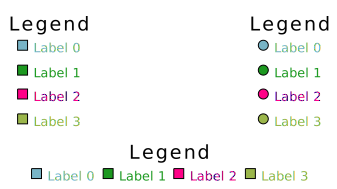
\includegraphics[keepaspectratio,width=\linewidth / 2,height=\fullh]{diagrams/legend.pdf}
\caption[Legend Example]{
  This is an example of three different legends that have been created from the source code in Listing~\ref{list:Legend}.
  One legend has been configured to have rectangles as symbols, one has been configured to have circles as symbols, and the last one has been configured with rectangle symbols but with horizontally laid out legend items.
  \imgcredit{Image created by the author of this thesis.}
}
\label{fig:Legend}
\end{figure}

ein data object mit welchem das rendering einer legende konfigurert werden kann wird durch das \code{Legend} interface beschrieben.
dieses interface beinhaltet ein \code{title} string property, ein \code{labels} string array property, ein \code{symbols} function oder function array property, ein \code{styleClasses} string oder string array property, und ein \code{keys} string array property.
der titel einer legende kann optional ueber das \code{title} property gesetzt werden.
das \code{labels} string array property definiert die labels neben den symbolen der einzelnen legend items.
die symbole der legend items werden ueber das \code{symbols} property bestimmt.
da die symbole einer legende komplett konfigurierbar sein sollen wird nicht einfach ein \code{<rect>} oder \code{<circle>} element als symbol gerendert sondern ein \code{<path>} element.
die verwendung eines \code{<path>} elementes ermoeglicht es beliebige symbole in der legende zu visualisieren.
der nachteil hiervon ist dass die konfiguration von \code{<path>} elementen aufwaendiger ist als die konfiguration von eingeschraenkteren SVG elementen.
das rendern eines symbols als \code{<path>} wird ueber eine funktion erledigt welche als input das jeweilige \code{<path>} element und die vom Layouter berechneten boundaries erhaelt.
in dem \code{symbols} property des \code{Legend} data objektes kann entweder eine einzelne solche funktion oder ein array von solchen funktionen gesetzt sein.
ist eine einzelne funktion gesetzt, erhaelt jedes symbol die selbe path konfiguration. 
sollte hier ein array an funktionen gesetzt sein, dann wird jedes symbol durch eine eigene path konfiguration visualisiert.
das \code{styleClasses} property erlaubt die konfiguration der style klassen von legend items.
eine style klasse wird in dem \code{data-style} attribut eines elementes gesetzt und dient der konfiguration von visuellen eigenschaften ueber CSS.
ein beispiel fuer verfuegbare style klassen sind die \code{categorical-0} bis \code{categorical-9} style klassen.
das setzen einer dieser klassen im \code{data-style} attribut eines elementes fuehrt dazu dass das CSS \code{fill} property auf die jeweilige kategorische farbe gesetzt wird.  
wird in dem \code{styleClasses} property eine einzelne style klasse deklariert, dann wird diese style klasse auf allen legend items gesetzt.
alternativ dazu akzeptiert dieses property auch ein array an style klassen, was dazu fuehrt das jedes legend item eine eigene style klasse gesetzt bekommt.
das \code{keys} property eines \code{Legend} data objektes bestimmt die werte der \code{data-key} attribute der einzelnen legend items.
ein data objekt das der form des \code{Legend} interface entspricht kann mit der \code{legendData} funktion erzeugt werden.
diese funktion erhaelt ein input objekt von dem selben typ wie jener den sie erzeugt bei welchem die werte die fuer den aufrufenden code nicht von interesse sind nicht gesetzt sein muessen und mit standardwerten befuellt werden.

eine legende wird mit der \code{legendRender} funktion auf elementen gerendert auf denen ein \code{Legend} data objekt gebunden ist.
diese funktion setzt die \code{legend} klasse auf den elementen der uebergebenen Selection.
innerhalb des root elementes der legende befindet sich ein \code{<text>} element mit der \code{text} klasse welches den titel der legende representiert, und ein \code{<g>} element mit der \code{items} klasse in welches die einzelnen legend items ueber einen data join gerendert werden.
um den legend item data join durchzufuehren benoetigt man ein data objekt pro legend item das gerendert werden soll.
dieses array an \code{LegendItem} data objekten, welche aus den \code{label}, \code{styleClass}, \code{symbol}, und \code{key} eigenschaften bestehen, wird durch transformation des \code{Legend} data objektes erzeugt.
ueber einen data join mit diesem array an data objekten wird fuer jedes legend item ein \code{<g>} element mit der \code{legend-item} klasse erzeugt.
an jedes dieser \code{<g>} elemente werden dann ein \code{<path>} element mit der \code{symbol} klasse und ein \code{<text>} element mit der \code{label} klassen angehaengt.
das \code{label} property des gebundenen \code{LegendItem} data objektes wird dann als textinhalt des \code{<text>} elementes gesetzt und das \code{symbol} property wird verwendet um die form des \code{<path>} objektes zu bestimmen.
ausserdem werden die \code{data-style} und \code{data-key} attribute auf dem \code{<g>} legend item element auf die werte der \code{styleClass} und \code{key} eigenschaften des data objektes gesetzt.
im kern kann eine legende auch als legend item series angesehen werden und wie auch alle anderen series components kann auch in den data join der legende direkt ueber die \code{enter}, \code{update}, und \code{exit} events, welche auf dem root element der legende gesendet werden, eingegriffen werden.
die event objekte dieser events beinhalten im \code{detail.selection} property jeweils die enter, update, und exit Selections des darunterliegenden data joins.
ueber diese properties koennen beliebige operationen in den verschiedenen phasen des data joins ausgefuehrt werden.


\TODO{Capitalize "Core Module", "Bar Module", "Chart", "Chart Component", "Axis", "Axis Component" according to Keith}




\section{Tooltip Module}
\label{sec:TooltipModule}

\TODO{Capitalize "Tooltip", "Tooltip Module", ...}

tooltips werden verwendet um zusaetzliche informationen eines elementes anzuzeigen die zu umfangreich sind um sie permanent anzuzeigen.
eine visualisierung die zu viele informationen zur selben zeit darstellt verliert an effektivitaet da ein groesserer kognitiver aufwand aufgebracht werden muss um sie zu interpretieren.
durch die verwendung von tooltips kann dieses problem dadurch geloest werden dass zu detailierte informationen erst durch interaktion der benutzter mit einem element in dessen kontext die information steht angezeigt werden.
ausserdem ist es fuer tooltips ok andere wichtige teile einer visualisierung zu ueberdecken da sie nicht permanent sichbar sind.
ein beispiel eines bar charts in welchem zusaetzliche informationen ueber einen tooltip angezeigt werden kann in Figure~\ref{fig:Tooltip} gesehen werden.

\begin{figure}[tp]
\centering
\includegraphics[keepaspectratio,width=\linewidth,height=\fullh]{images/tooltip.png}
\caption[Tooltip Example]{
  A bar chart with a tooltip showing additional information of the data record associated with an individual bar.
  Since the tooltip is only visible while the user interacts with the context element, it is ok that the tooltip covers other important parts of the visualization.
  \imgcredit{Image created by the author of this thesis.}
  }
  \label{fig:Tooltip}
\end{figure}
  
  
das tooltip module befindet sich im \code{src/lib/tooltip/} odner des projektes.
die hauptdatei welche die implementierung der tooltip funktionalitaet beinhaltet ist die \code{tooltip.ts} datei.
so wie tooltips hier implementiert wurden, wird die gleichzeitige anzeige mehrerer tooltips unterstuetzt.
um dies zu erreichen, erwarten alle funktionen die tooltip operationen ausfuehren, dass das tooltip element auf welchem die operation ausgefuehrt werden soll als erster parameter an die funktion uebergeben wird.
diese funktionen erlauben es allerdings auch ein \code{null} objekt in diesem parameter zu uebergeben, was zur verwendung eines standard tooltip elementes, welches an das \code{<body>} element des aktiven dokumentes angehaengt wird, fuehrt.
%
tooltips sind HTML \code{<div>} elemente mit der \code{tooltip} klasse und werden ueber CSS gestyled.
der inhalt eines tooltips wird mit der \code{tooltipContent} funktion gesetzt.
diese funktion erlaubt es den inhalt eines tooltips als string zu definieren welcher als HTML inhalt des tooltip elementes gesetzt wird.
%
die position eines tooltips wird ueber die \code{tooltipPosition} funktion gesetzt.
diese funktion erhaelt ein objekt als parameter mit welchem die position in viewport koordinaten und ein optionaler offset von dieser position bestimmt werden.
wird kein expliziter offset gefordert berechnet die \code{tooltipPosition} funktion einen welcher den tooltip so postioniert dass er immer in dem sichtbaren bereich des browsers positioniert wird.
tooltips werden ueber viewport koordinaten positioniert und die endgueltige position eines tooltips wird ueber die CSS \code{top}, \code{bottom}, \code{left}, und \code{right} eigenschaften gesetzt.
welche dieser eigenschaften verwendet wird haengt von der offset richtung des tooltips ab. 
%
tooltips werden mit der \code{tooltipShow} funktion angezeigt und mit der \code{tooltipHide} funktion versteckt.
diese funktionen setzen und enfernen jeweils die \code{show} klasse von dem tooltip element wodurch die CSS \code{opacity} eigenschaft des elementes beinflusst wird. 

neben der \code{tooltip.ts} datei beinhaltet das tooltip modul noch die \code{series-config-tooltips.ts} datei.
in dieser datei befindet sich keine eigene komponente sondern utility funktionen um die konfiguration und das handling von tooltips auf series komponenten zu vereinfachen.
die datenobjekt interfaces von series komponenten mit welchen tooltips konfiguriert werden sollen koennen von dem \code{SeriesConfigTooltips} interface erben.
dieses interface beinhaltet die \code{tooltipsEnabled}, \code{tooltips}, und \code{tooltipPositions} eigenschaften.
die \code{tooltipsEnabled} boolean eigenschaft ermoeglicht das aktivieren und deaktivieren von tooltips.
der inhalt der tooltips von individuellen series item elements wird ueber die \code{tooltips} eigenschaft konfiguriert.
in dieser eigenschaft wird eine funktion gesetzt die mit dem series item element aufgerufen wird fuer welches ein tooltip angezeigt werden soll und welche den tooltipinhalt als string zurueckliefert.     
die positionen der einzelnen tooltips werden ueber die \code{tooltipPositions} eigenschaft gesetzt.
der wert dieser eigenschaft ist ebenfalls eine funktion welche mit dem kontext series item element und der aktuellen mausposition in viewport koordinaten als parameter aufgerufen wird.
die gewuenschte position des tooltips kann dann ueber diese parameter berechnet werden.
%
zusaetzlich zu dem \code{SeriesConfigTooltips} interface kann die \code{seriesConfigTooltipsHandleEvents} funktion in der \code{series-config-tooltips.ts} datei gefunden werden.
diese funktion kann in series komponenten verwendet werden um \code{mouseover}, \code{mousemove}, und \code{mouseout} event listener an die root elemente einer series anzuhaengen die fuer das management von tooltips zustaendig sind.
diese event listener verwenden die \code{SeriesConfigTooltips} eigenschaften der an den series elementen gebundenen datenobjekte um die sichtbarkeit, den inhalt, und die position von tooltips zu modifizieren.
die verwendung dieser utility typen und funktionen ist optional.
es steht series komponenten frei eigene eigenschaften fuer die konfiguration von tooltips zur verfuegung zu stellen und das handling von tooltips selbst zu implementieren.
allerdings ist es aus konsistenzgruenden besser wenn sich die art der konfiguration von tooltips nicht zu sehr zwischen unterschiedlichen series komponenten unterscheidet.   



\section{Bar Module}

das bar modul befindet sich in dem \code{src/lib/bars/} ordner des projektes und beinhaltet komponenten um unterschiedliche arten von bar charts zu rendern.
bar charts werden zur visualisierung von kategorischen datensaetzen durch rectangles eingesetzt wobei die laenge der rectangles proportional zu den werten einer quantitativen datendimension ist.
in einem kategorischen datensatz ist eine kategorie eindeutig anderen dimensionen der einzelnen dateneintraege zuordenbar.
ein beispiel hierfuer waere ein datensatz in welchem unterschiedliche charakteristiken einzelner laender aufgelistet sind.
bar charts gehoeren zu den aeltesten arten von charts mit einem der ersten aufkommen in \textcite{CommercialAndPoliticalAtlas} und gehoeren auch heute noch zu den am haeufigsten vorgefundenen visualisierungen (~36\% der 378 studied charts by \textcite{DesignPatternsTradeOffsRespVisGallery}) im modernen web.
die bars einens bar charts koennen entweder horizontal oder vertikal ausgerichtet sein.
bei einem horizontalen bar chart, manchal auch row chart genannt, wird die quantitative dimension ueber die X achse ausgedrueckt.
diese variante von bar charts eignet sich besser fuer die darstellung in layouts mit eingeschraenkter breite, da die labels der kategorischen achse leichter ohne zu ueberlappen positioniert werden koennen und da ein horizontaler bar chart vertikal gescrollt werden kann was horizontalem scrollen zu bevorzugen ist.
im gegensatz zu horizontalen bar charts wird bei vertikalen bar charts, manchmal auch column charts genannt, die quantitative dimension ueber die Y achse ausgedrueckt. 
das bar modul beinhaltet komponenten fuer das rendering von basic, grouped, und stacked bar charts welche in unterschiedlichen visualisierungsszenarien eingesetzt werden koennen.
fuer jede art von bar chart wird eine Series Component, eine Chart Component und eine Chart Window Component zur verfuegung gestellt. 
die implementierung der unterschiedlichen arten von bar charts und wann welche art am besten zur anwendung kommt wird in den folgenden sections beschrieben.

\subsection{Basic Bars}

\TODO{Is "Basic Bars" a good name? Maybe "Single Bars" or "Bars" or something else?}

\TODO{Add figure of vertical and horizontal bar charts (subfigures?)}

basic bar charts, manchmal auch single-series bar charts genannt, werden verwendet um unterschiede einer quantitativen dimension verschiedener kategorien eines kategorischen datensatzes zu verdeutlichen.
von jedem dateneintrag wird jeweils eine kategorische und eine quantitative dimension als eine bar visualisiert, wobei die zu visualisierenden kategorien eindeutig auf einen quantitativen wert gemapped werden koennen muessen.
die kategorien eines bar charts werden ueber eine band scale auf raeumliche dimensionen gemapped.
eine band scale wird verwendet um werte gleichmaessig auf gleich grosse intervalle (baender) des verfuegbaren platzes aufzuteilen. 
der abstand zwischen den einzelnen intervallen ist konfigurierbar.
die breite der zu rendernden bars ergibt sich durch die anzahl der kategorien, dem bereich auf welchen sie ueber die band scale aufgeteilt werden sollen, und dem abstand zwischen den bars. 
die quantitativen werte, welche die laenge der individuellen bars bestimmen, werden ueber eine continuous scale auf raemliche dimensionen gemapped.
eine continuous scale bildet abstrakte quantitative werte ueber eine kontinuierliche interpolationsfunktion auf den bereich zwischen zwei extemen ab.
in den meisten faellen kommt eine lineare interpolation ueber eine linear scale zur anwendung.
es steht dem author einer visualisierung jedoch frei eine andere form der interpolation, wie zum beispiel eine logarithmische funktion ueber eine logarithmic scale, zu waehlen. 

die lowest-level komponente die fuer das rendern eines bar charts notwendig ist ist eine bar series.
eine bar series ist eine sammlung von \code{<rect>} elementen welche die bars innerhalb der draw area eines bar charts representieren.
die implementierung der bar series komponente befindet sich in der \code{series-bar.ts} datei des bar moduls.
das datenobjekt fuer die konfiguration einer bar series wird ueber das \code{SeriesBar} interface beschrieben.
diese interface beschreibt ein objekt mit den \code{categories}, \code{values}, \code{categoryScale}, \code{valueScale}, \code{flipped}, \code{styleClasses}, und \code{keys} eigenschaften.
zusaetzlich zu diesen eigenschaften wird die konfiguration von tooltips ueber die eigenschaften des \code{SeriesConfigTooltips} interface, welches in Section~\ref{sec:TooltipModule} beschrieben wird, ermoeglicht.
die \code{categories} und \code{values} eigenschaften sind arrays welche die individuellen kategorien und deren quantitative werte repraesentieren.
das mapping der kategorischen und quantitativen werte auf raeumliche dimensionen wird ueber die \code{categoryScale} und \code{valueScale} eigenschaften bestimmt.
ob vertikale oder horizontale bars gerendert werden haengt von dem wert der \code{flipped} eigenschaft ab, wobei ein wert von \code{false} fuer vertikale bars und ein wert von \code{true} fuer horizontale bars steht.
die \code{data-style} attribute, welche die farbe von bars bestimmen, und die \code{data-key} attribute, welche zur identifikation von zusammengehoerenden elementen verwendet werden, werden ueber die \code{styleClasses} und \code{keys} eigenschaften bestimmt.
ein mit standardwerten initialisiertes \code{SeriesBar} datenobjekt kann mit der \code{seriesBarData} funktion von einem partiellen input objekt erzeugt werden.
diese datenobjekte koennen an \code{<svg>} oder \code{<g>} elemente gebunden werden in welche dann eine bar series mit der \code{seriesBarRender} funktion gerendert werden kann.
die individuellen bar elemente werden ueber einen data join mit einem array an \code{Bar} datenobjekten erzeugt, welches durch transformation des gebundenen \code{SeriesBar} datenobjektes berechnet wird.
die position und groesse der bars wird mithilfe der beiden scales berechnet deren output values auf die dimensionen der bounding box des series elementes gemapped werden, welche vom Layouter berechnet und im \code{bounds} attribut gespeichert wurden.
jede bar hat eine enter und exit transition und ihre position und groesse wird ueber eine update transition zwischen aktuellen und neuen werten interpoliert.
diese transitions erleichtern es aenderungen in den visualisierten daten nachzuvollziehen und fuehren zu einer verbesserung der user experience.
wie bei alle anderen series komponenten, werden die enter, update, und exit events mit der jeweiligen Selection des bar data joins auf dem root element der series dispatched um das injezieren von eigenem verhalten in die verschiedenen phasen des data joins zu ermoeglichen. 

die implementierung von bar charts befindet sich in der \code{chart-bar.ts} datei im bar modul. 
bar charts sind kartesische charts die eine bar series mit optionalen labels in ihrer draw area rendern.
das \code{ChartBar} interface beschreibt die form von datenobjekten fuer die konfiguration von bar charts.
es beinhaltet alle eigenschaften der \code{ChartCartesian} und \code{SeriesBar} interfaces und fuegt zusaetzliche eigenschaften zur konfiguration von bar labels hinzu. 
ein mit standardwerten initialisiertes datenobjekt vom typ \code{ChartBar} kann mit der \code{chartBarData} funktion von einem partiellen input objekt erzeugt werden.
nachdem solch ein datenobjekt auf einem \code{<svg>} oder \code{<g>} element gebunden wurde, kann ein bar chart mit der \code{chartBarRender} funktion in dieses element gerendert werden.
diese funktion initialisiert einen kartesischen chart, initialisiert und rendert eine bar series und eine optionale label series in der draw area des charts, und rendert die scales mit welchen die bar series gerendert wurde als left und bottom axes des charts. 
weiters werden \code{mouseover} event listener an die bar series angehaengt die fuer das hervorheben von bars und den dazugehoerigen ticks auf der category axis zustaendig sind.

ein bar chart window ist die highest-level komponente die verwendet werden kann um einen bar chart zu rendern der in ein Layouter element eingebettet wird um dessen elemente ueber CSS zu positionieren.
ueber die toolbar des bar chart windows koennen die kategorien des bar charts gefiltert und das SVG dokument des bar charts gedownloaded werden.
das datenobjekt fuer die konfiguration eines bar chart windows wird durch das \code{ChartWindowBar} interface beschrieben.
dieses interface erbt vom \code{ChartBar} interface und beinhaltet dadurch alle eigenschaften die fuer die konfiguration des darunterliegenden bar charts benoetigt werden.
zusaetzlich zu diesen, werden weitere eigenschaften fuer das filtern von kategorien, wie etwa die derzeit aktiven kategorien und das verhalten der value scale, zur verfuegung gestellt.
die \code{chartWindowBarData} funktion kann verwendet werden um ein datenobjekt fuer die konfiguration eines bar chart windows von einem partiellen input objekt zu erzeugen bei welchem die nicht definierten werte mit standardwerten initialisiert werden.
mit der \code{chartWindowBarRender} funktion kann ein bar chart window in einem \code{<div>} element auf welchem ein angemessenes datenobjekt gebunden is gerendert werden.
diese funktion rendert die toolbar mit den kategorie filter und SVG download tools, initialisiert den eingebetteten chart mit den gefilterten werten des chart window datenobjektes, und rendert den chart, entsprechend des render prozesses definiert in Section~\ref{sec:Layouter}, zweimal mit einem layout computation schritt dazwischen.
standardmaessig wird das chart window nicht automatisch rerendert wenn sich die groesse des viewports aendert oder wenn die aktiven kategorien gefiltert werden.
das rerendern bei viewport groessenaenderungen kann ueber einen \code{resize} event listener auf dem chart window root element implementiert werden in welchem die chart window render funktion erneut aufgerufen wird nachdem das gebundene datenobjekt angemessen an die neuen dimensionen des viewports angepasst wurde.
das bar chart window sendet ein \code{categoryfilter} event mit den derzeit aktiven kategorien immer wenn kategorien ueber das filter tool aktiviert oder deaktiviert werden.
um den bar chart auf die neue filterkonfiguration anzupassen muss ein \code{categoryfilter} event listener implementiert werden welcher die aktiven kategorien im datenobjekt des chart windows aktualisiert und das chart window rerendert.
muessen keine speziellen konfigurationen bei aenderung der viewport groesse oder des kategoriefilters durchgefuehrt werden, koennen die \code{chartWindowBarAutoResize} und \code{chartWindowBarAutoFilterCategories} funktionen verwendet werden um \code{resize} und \code{categoryfilter} event listener an das chart window anzuhaengen die das standardverhalten implementieren.
ein simples beispiel dafuer wie ein skalierendes bar chart window erzeugt werden kann welches das filtern von kategorien erlaubt ist in Listing~\ref{list:BarChartWindow} ersichtlich.
die resultierende visualisierung dieses codes kann in Figure~\ref{fig:BarChartWindow} gesehen werden.

\begin{samepage}
\lstinputlisting[%
  float=tp,
  aboveskip=\floatsep,
  belowskip=\floatsep,
  xleftmargin=0cm,              % no extra margins for floats
  xrightmargin=0cm,             % no extra margins for floats
  %
  basicstyle=\footnotesize\ttfamily,
  frame=shadowbox,
  numbers=left,
  label=list:BarChartWindow,
  caption={[Basic Bar Chart Window Example]%
    The example source code that creates a basic Bar Chart Window.
    The Bar Chart Window is configured with the bound data object that is initialized via the \code{chartWindowBarData} function.
    After configuration, the Chart Window is rendered by the \code{chartWindowBarRender} function.
    Since no special responsive behavior is desired in this example, the default resize and category filter behavior is attached to the Chart Window via the \code{chartWindowBarAutoResize} and \code{chartWindowBarAutoFilterCategories} functions. 
  },
]{listings/bar-chart-window.js}
\end{samepage}
  

\begin{figure}[tp]
\centering
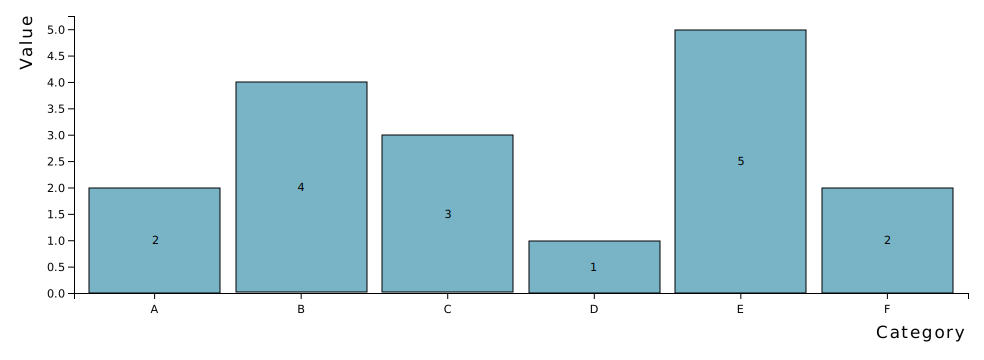
\includegraphics[keepaspectratio,width=\linewidth,height=\fullh]{images/bar-chart-window.png}
\caption[Basic Bar Chart Window Example]{
  The resulting Bar Chart of the example code in Listing~\ref{list:BarChartWindow}. 
  \imgcredit{Image created by the author of this thesis using RespVis and \href{https://inkscape.org/}{Inkscape}.}
}
\label{fig:BarChartWindow}
\end{figure}



\subsection{Grouped Bars}

ein grouped bar chart, manchmal auch clustered oder multi-series bar chart genannt, wird verwendet um mehrere quantitative dimensionen unterschiedlicher kategorien eines kategorischen datensatzes miteinander zu vergleichen.
in einem solchen chart wird fuer jede kategorie eine gruppe an bars gerendert deren laengen proportional zu den werten der unterschiedlichen quantitativen dimensionen sind.
die verschiedenen zu visualisierenden quantitativen dimensionen muessen miteinander vergleichbar sein und koennen als unterkategorien der einzelnen kategorien betrachtet werden.
wie bei basic bar charts werden auch hier die kategorien ueber band scales auf raeumliche dimensionen abgebildet.
der unterschied befindet sich darin dass bei grouped bar charts zwei verschiedene band scales zur anwendung kommen.
ueber die category scale wird der verfuegbare platz der draw area auf die anzahl der kategorien aufgeteilt und ueber die subcategory scale wird der platz innerhalb der daraus resultierenden gleich grossen intervalle auf die anzahl der unterkategorien aufgeteilt.
das abbilden von quantitativen werten auf raeumliche dimensionen wird wieder ueber eine continuous scale durchgefuehrt, wobei die selbe scale fuer jeden wert verwendet werden muss damit die werte miteinander vergleichbar sind.

fuer das rendering von grouped bar charts werden drei verschiedene komponenten zur verfuegung gestellt welche ihren gegenstuecken fuer das rendering von basic bar charts sehr aehnlich sind.
die grouped bar series ist die lowest-level komponente die dafuer gedacht ist eine sammlung an \code{<rect>} elementen, welche die jeweiligen werte und kategorien eines grouped bar charts representieren, in die draw area eines charts zu rendern.
der unterschied einer grouped bar series zu einer basic bar series ist dass zusaetzliche eigenschaften fuer die konfiguration der unterkategorien notwendig sind und dass manche bereits vorhandene eigenschaften hier zwei-dimensionale arrays erfordern um deren werte den hier zwei-dimensional (kategorie/unterkategorie) gruppierten bars zuzuordnen.
allen bars die der selben unterkategorie angehoeren werden die selben style klassen zugewiesen um die werte der einzelnen kategorien leichter miteinander vergleichen zu koennen.
ein grouped bar chart ist ein kartesischer chart mit einer grouped bar series und optionalen labels in seiner draw area, einer left und bottom axis die die scales der grouped bar series visualisieren, und einer legende die die unterkategorien des charts beschreibt.
ein solcher Chart implementiert ausserdem event listener auf unterschiedlichen elementen die das gemeinsame hervorheben von zusammengehoerenden bars, labels, category axis ticks, und legend items abwickeln.  
ein Grouped Bar Chart Window ist die highest-order komponente die verwendet werden kann um einen Grouped Bar Chart zu rendern.
diese komponente plaziert den Chart innerhalb eines Layouters und managed den render prozess der es erlaubt individuelle elemente ueber CSS zu positionieren.
weiters dekoriert ein solches Chart Window den Grouped Bar Chart mit einer toolbar in welcher sich ein SVG download tool und zwei filter tools befinden um die visualisierten kategorien und unterkategorien zu filtern.
die konfiguration des eingebetteten Charts mit den gefilterten eigenschaften des am Chart Window gebundenen datenobjektes wird von der render funktion des Grouped Chart Windows durchgefuehrt.
immer wenn der user mit den filter tools interagiert und die zusammenstellung der aktiven kategorien und unterkategorien veraendert werden die \code{categoryfilter} und \code{subcategoryfilter} events mit jeweils den neuen aktiven kategorien und unterkategorien ausgesandt.
der author der visualisierung kann entweder spezielles verhalten in eigenen resize und filter event listenern implementieren oder das standardverhalten ueber die zur verfuegung gestellten \code{chartWindowBarGroupedAutoResize}, \code{chartWindowBarGroupedAutoFilterCategories}, und \code{chartWindowBarGroupedAutoSubcategories} funktionen aktivieren.
der beispielcode um einen einfachen grouped bar chart zu erzeugen welcher sich an die groesse seines container elementes anpasst und in welchem die kategorien und unterkategorien ueber die toolbar gefiltert werden koennen befindet sich in Listing~\ref{list:GroupedBarChartWindow}.
die resultierende visualisierung dieses beispiels kann in Figure~\ref{fig:GroupedBarChartWindow} gesehen werden.  

\begin{samepage}
\lstinputlisting[%
  float=tp,
  aboveskip=\floatsep,
  belowskip=\floatsep,
  xleftmargin=0cm,              % no extra margins for floats
  xrightmargin=0cm,             % no extra margins for floats
  %
  basicstyle=\footnotesize\ttfamily,
  frame=shadowbox,
  numbers=left,
  label=list:GroupedBarChartWindow,
  caption={[Basic Grouped Bar Chart Window Example]%
    The example source code that creates a basic Grouped Bar Chart Window.
    The Grouped Bar Chart Window is configured with the bound data object that is initialized via the \code{chartWindowBarGroupedData} function.
    After configuration, the Chart Window is rendered by the \code{chartWindowBarGroupedRender} function.
    Since no special responsive behavior is desired in this example, the default resize, category filter, and subcategory filter behavior is attached to the Chart Window via the \code{chartWindowBarAutoResize}, \code{chartWindowBarAutoFilterCategories}, and \code{chartWindowBarAutoFilterSubcategories} functions. 
  },
]{listings/grouped-bar-chart-window.js}
\end{samepage}
    
  
\begin{figure}[tp]
\centering
\includegraphics[keepaspectratio,width=\linewidth,height=\fullh]{images/grouped-bar-chart-window.png}
\caption[Basic Grouped Bar Chart Window Example]{
  The resulting Grouped Bar Chart of the example code in Listing~\ref{list:GroupedBarChartWindow}. 
  The tool menu popup has manually been displaced to not cover the legend. 
  \imgcredit{Image created by the author of this thesis using RespVis and \href{https://inkscape.org/}{Inkscape}.}
}
\label{fig:GroupedBarChartWindow}
\end{figure}

\subsection{Stacked Bars}



\section{Point Module}     

\cleardoublepage
\chapter{Examples}
\label{chap:Examples}

\section{Bar Chart}

\section{Grouped Bar Chart}

\section{Stacked Bar Chart}

\section{Scatterplot}

\TODO{Write about application example (newspaper article?)} 

\cleardoublepage
%----------------------------------------------------------------
%
%  File    :  thesis-details.tex
%
%  Author  :  Keith Andrews, IICM, TU Graz, Austria
% 
%  Created :  17 Nov 2004
% 
%  Changed :  17 Nov 2004
% 
%----------------------------------------------------------------

\chapter{Selected Details of the Implementation
(and Test of Extremely
Long Chapter Titles to See How They Work or Not)
}

\label{chap:SelectedDetails}


\chapquote{
The devil is in the detail.
}
{
English proverb.
}


There are often specific details of a project, which involve
particularly much work to get right, but do not form a major part in
the whole scheme of things, so would not generally deserve a chapter
of their own. This chapter is for these details.



\section{First Selected Detail}

The context, the decision process, all the variations that were tried,
and the solution that was finally adopted.



\section{Second Selected Detail}

From some other part of the project. Explaining your reasoning and
choices will help some other poor student, who has to pick up your
work from where you left off.



\section{Using a Table}

An example of using a table can be seen in Table~\ref{tab:BestPubs}.

\begin{table}[tp]
\centering
\begin{tabularx}{\linewidth}{|llrX|}
\hline
Name & Type & Rating & Description \\
\hline
Flann O'Brien &
Irish &
***** &
In the centre of town and easy to find for
marauding tourists. Very smooth Guinness.
\\
\hline
The Office &
English &
***** &
Hidden in the narrow streets of the old town.
Erasmus student night every other Wednesday.
\\
\hline
O'Carolans &
Irish &
*** &
In the centre of town in a small side street next to Flann's.
Small, cosy, but hellishly smoky.
\\
\hline
O'Riginal &
pseudo Irish &
 &
Austrian dive pretending to be an Irish pub.
\\
\hline
\end{tabularx}

\caption[Best Pubs in Graz]
{
The best pubs in Graz.
}
\label{tab:BestPubs}
\end{table}





\section{Using Subfigures}

This example shows how to include vector graphics in the form of PDF
files. It also shows how to use subfigures within a figure.

\begin{figure}[tp]
\centering
\subfloat[][%  the % chars remove implicit spacing
An object has been composed to represent an
abstract version of the clock tower in Graz.
Here, the object is in its initial state.
]
{%
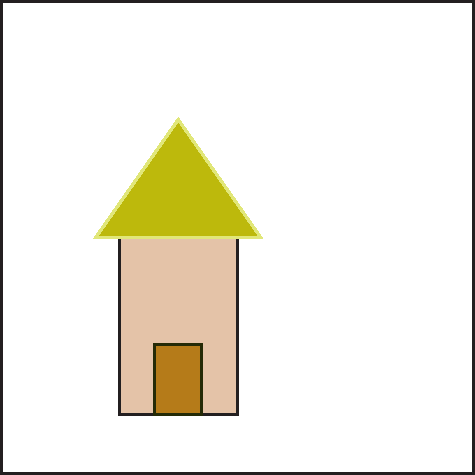
\includegraphics[width=0.45\linewidth]
{diagrams/multi1.pdf}%
\label{fig:Tower1}%
}
\hfill
\subfloat[][%
The object has been scaled and rotated, and now resembles
a leaning tower.
]
{%
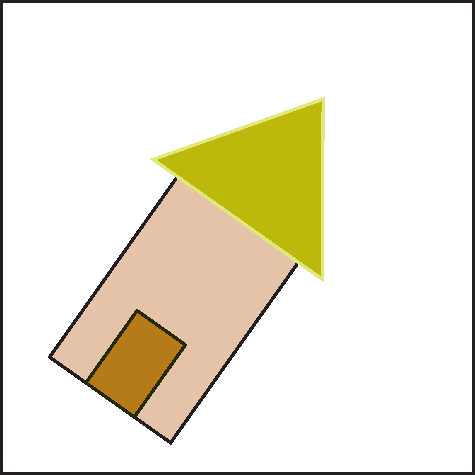
\includegraphics[width=0.45\linewidth]
{diagrams/multi2.pdf}%
\label{fig:Tower2}%
}

\caption[Abstract Clock Towers]
{
The leaning tower of Graz. An abstract model of the clock
tower in Graz leaning over time. \subref{fig:Tower1} shows
the initial state. \subref{fig:Tower2} shows the final state.
\imgcredit{Both images created by the author of this thesis.}
}
\label{fig:WholeFig}
\end{figure}


An example of using the \vname{subfig} package can be seen in
Figure~\ref{fig:WholeFig}. Figure~\ref{fig:Tower1} shows the polygons
before transformation, while Figure~\ref{fig:Tower2} shows them
afterwards.





\section{Including a Screenshot}

This example shows how to include a screenshot (or other raster
graphic) into a \LaTeXe\ figure.

\begin{figure}[tp]
\centering
\includegraphics[keepaspectratio,width=\linewidth,height=\halfh]
{images/pist.png}

\caption[VRwave in Flip Mode]
{%
VRwave in Flip mode displaying a textured model of a cavalry pistol
from the world-renowned Zeughaus (armoury) in Graz.
\imgcredit{Image extracted from \textcite[page~81]{Andrews-VRwave}
and used under the terms of the ACM Copyright Policy. \copyrightACM}
}
\label{fig:Pistol}
\end{figure}


An example of how to correctly cite the source when using an image
from someone else. In their 1998 paper, \textcite{Andrews-VRwave}
discuss the VRwave VRML browser. Figure~\ref{fig:Pistol} shows a VRML
model of a cavalry pistol from the Armoury in Graz displayed in the
VRwave VRML browser.





\section{Using Special Characters and Symbols}

You can use many (but not all) of the thousands of characters
available in the UTF-8 \parencites{Wikipedia-UTF8}{Unicode-Charts}
character encoding. For example, the German umlauts (äüö), the German
sharp s (ß), or the yen symbol (¥).

You can also try some of the \approxsym 100 symbols available
in the \vname{textcomp} package, such as the yen symbol (\textyen) and
a circled letter A (\textcircled{A}).



\section{Using Macros to Style Special Names}

Use the \vname{vname}, \vname{cname}, and \vname{fname} macros to
define the style for (say) variable names, class names, and file
names. You can also define your own macros. The is a very long file
name \fname{/usr/data/keith/travel/austria/vienna.txt} to see how they
are broken at a line end. A typical class name is
\cname{HVSInformationPyramidsInputFactory}.





\section{Using Macros as Shorthand}

Sometimes, a macro (new command definition) can be useful to define
the contents of table cells, particularly if these contain images. For
example, Table~\ref{tab:WinIconicLang} uses the macro called
\vname{iibox}, which takes a single parameter, the name of
the particular image.


\begin{table}[tp]

\newcommand{\iibox}[1]{\parbox[c][1cm][c]{1cm}{%
\includegraphics[scale=0.6]{./images/icons/#1.png}
}}

\begin{center}
\begin{tabular}[t]{|p{7cm}c|}
\hline
\multicolumn{2}{|l|}{\sffamily \bfseries Elementary Symbols}            \\
Document                            & \iibox{win-il-gen-doc}            \\
Assistant                           & \iibox{win-il-gen-ass}            \\
Template                            & \iibox{win-il-gen-tmpl}           \\
\hline
\multicolumn{2}{|l|}{\sffamily \bfseries Document Types}                \\
Text document                       & \iibox{win-il-text-doc}           \\
Spreadsheet document                & \iibox{win-il-spreadsheet-doc}    \\
Presentation document               & \iibox{win-il-presentation-doc}   \\
Database document                   & \iibox{win-il-database-doc}       \\
\hline
\multicolumn{2}{|l|}{\sffamily \bfseries Applications}                  \\
Word                                & \iibox{win-il-word-appl}          \\
Excel                               & \iibox{win-il-xls-appl}           \\
Powerpoint                          & \iibox{win-il-ppt-appl}           \\
Access                              & \iibox{win-il-mdb-appl}           \\
\hline
\multicolumn{2}{|l|}{\sffamily \bfseries Generated Icons}               \\
Word text document                  & \iibox{win-il-word-doc}           \\
Excel spreadsheet document          & \iibox{win-il-xls-doc}            \\
Powerpoint presentation document    & \iibox{win-il-ppt-doc}            \\
Access database document            & \iibox{win-il-mdb-doc}            \\[2ex]
%
Word template                       & \iibox{win-il-word-tmpl}          \\
Powerpoint template                 & \iibox{win-il-ppt-tmpl}           \\
Access template                     & \iibox{win-il-mdb-tmpl}           \\[2ex]
%
Word template assistant             & \iibox{win-il-word-ass}           \\
Powerpoint template assistant       & \iibox{win-il-ppt-ass}            \\
Access template assistant           & \iibox{win-il-mdb-ass}            \\[2ex]
%
\hline
\end{tabular}
\end{center}

\caption[Iconic language for Windows NT 4.0 documents]
{
Iconic language for Windows NT 4.0 documents.
\imgcredit{The icons are screenshots, captured and then
enlarged by the author of this thesis.}
}
\label{tab:WinIconicLang}
\end{table}







\begin{samepage}
\begin{lstlisting}[%
  float=tp,
  aboveskip=\floatsep,
  belowskip=\floatsep,
  xleftmargin=0cm,              % no extra margins for floats
  xrightmargin=0cm,             % no extra margins for floats
  basicstyle=\footnotesize\ttfamily,
  frame=shadowbox,
  numbers=left,
  language=HTML,
  label=list:HTML5Boilerplate,
  caption={[HTML5 Boilerplate Code]%
Some HTML5 boilerplate code, illustrating the typical structure
of a HTML5 web page.
},
]
<!DOCTYPE html>
<html xmlns="http://www.w3.org/1999/xhtml" lang="en" xml:lang="en">

<head>
<meta charset="UTF-8"/>
<meta name="viewport" content="width=device-width, initial-scale=1"/>
<link rel="stylesheet" href="./inm.css"/>

<title>Keith Andrews Web Page</title>
</head>

<body>

<header>
<img src="images/kalogo.svg" alt="KA Logo"/>
Keith Andrews Design
</header>

<h1>Keith Andrews</h1>

<p>
Keith lives in <a href="http://graz.at/">Graz</a>.
</p>

<p>
<img src="images/keith-s.jpg"
  alt="Photo of Keith Andrews"/>
</p>

<p>
Three desirable attributes:
</p>
<ol>
<li>cheap</li>
<li>fast</li>
<li>good</li>
</ol>
<p>
Choose any two.
</p>

<p>
<abbr title="Extensible HyperText Markup Language">XHTML</abbr>
is cool.
</p>

<table>
<tbody>
<tr><th>Beer</th><th>Price €</th></tr>
<tr><td>Puntigamer</td><td>2,60</td></tr>
<tr><td>Gösser</td><td>2,60</td></tr>
<tr><td>Guinness</td><td>4,35</td></tr>
</tbody>
</table>

<footer>
Copyright © Keith Andrews 2019.
</footer>

</body>
</html>
\end{lstlisting}
\end{samepage}



\section{Using Floating Listings}

Listing~\ref{list:HTML5Boilerplate} is floating. A floating listing is
a block of code treated like other \LaTeXe floats (such as figures or
tables). Use floating listings for longer blocks of code.
A floating listing is given a number and can be referred to
explicitly, like Listing~\ref{list:HTML5Boilerplate}. It can be given
a caption and short caption, and is listed in the List of Listings.





\section{Using Non-Floating Diplayed Listings}

The listing below shows some CSS:
\begin{samepage}
\begin{lstlisting}[%
  language=CSS,
]
body { color: black; background-color: silver; }
img { border: none; }
h1,h2 { font-family: Verdana, sans-serif; }
\end{lstlisting}
\end{samepage}
It is displayed (i.e. indented as a block) in-place, but is not
floating. It cannot be referred to by number and is not listed in the
List of Listings. As a rule of thumb, if listings have five or more
lines, make them floating.





\section{Using Inline Listings}

Inline listings are used for very short snippets of code embedded
within the flow of a paragraph. For example,
\lstinline|\lstinline!var i:integer;!|
produces
\lstinline!var i:integer;!, which can now be discussed further.
Do not break an inline listing over multiple lines (EOL).




\section{Using Lists}

A list should always be introduced by a sentence
which ends with a colon.
%
There are three kinds of standard lists in \LaTeXe:
\begin{itemize}
\item itemize
\item enumerate
\item description
\end{itemize}
% A blank line here would indicate a new (indented) paragraph
An enumerated list has numbered items:
\begin{enumerate}
\item Fast
\item Good
\item Cheap
\end{enumerate}
Choose any two!


A description list has named items with corresponding
definitions or descriptions:
\begin{description}
\item[Short] Each item has a label (name) and its description.

\item[Rather longer label] By default, if the description text
  is rather long, it will warp around to the following lines.
\end{description}



     

\cleardoublepage
\chapter{Outlook and Future Work}

\label{chap:Outlook}


\section{Outlook}

\section{Ideas for Future Work}

\subsection{Post-Processing SVG String Before Download}

% newlines
% remove data attributes?

\subsection{Relative Positioning of Series Items}

\TODO{Write about plans to use relative units (\%) to position series items which would most likely get rid of the need to update components on bound changes}

\subsection{Container Queries}        

\cleardoublepage
%----------------------------------------------------------------
%
%  File    :  thesis-concl.tex
%
%  Author  :  Keith Andrews, IICM, TU Graz, Austria
% 
%  Created :  22 Feb 96
% 
%  Changed :  19 Feb 2004
% 
%----------------------------------------------------------------


\chapter{Concluding Remarks}

\label{chap:Concl}


\chapquote{
Everything has an end, only a sausage has two \\
(Alles hat ein Ende nur die Wurst hat zwei).
}
{
German, Danish, and Dutch proverb.
}



This thesis presented research work in the field of writing a thesis.
The concluding remarks should summarise the contents of the thesis and
underline what is new and original (i.e. the thesis' contribution to
academic progress). This is the opportunity to ``market'' the thesis
and its contributions.

The first chapter introduced the field. Chapters~\ref{chap:Struc} and
\ref{chap:Academic} covered the topics of structuring and preparing an
academic thesis.
%
Chapter~\ref{chap:Style} discussed styles of writing in English. Of
particular note, Section~\ref{sec:EnglishUsage} includes a collated
collection of mistakes often made by non-native English speakers in
computer science Master's theses. Chapter~\ref{chap:Presentation}
provided guidance for giving academic presentations.
Chapter~\ref{chap:Tech} outlined requirements and issues for the
technical production of a thesis. Chapter~\ref{chap:SelectedDetails}
covered specific details of the project which warranted closer
examination.
%
Finally, in Chapter~\ref{chap:Outlook}, the thesis concluded with an
analysis of current trends, an outline of work in progress,
and some ideas for future research.

       

\appendix

\cleardoublepage
\chapter{User Guide}

\label{app:UserGuide}           % Appendix A

\cleardoublepage
\chapter{Developer Guide}
\label{app:DeveloperGuide}
      % Appendix B



\backmatter

% Ensure that certain references are listed in the bibliography,
% even if they are not cited anywhere in the text.
% \nocite{KeithMastersThesis}
% \nocite{KeithPhdThesis}


\cleardoublepage
% for now, switch to language english
% hack to force unix date for biblio, biblatex 3.11
\begin{otherlanguage}{english}
  \printbibliography[heading=bibintoc]
\end{otherlanguage}



% \cleardoublepage
% \input{glossary}      % Glossary

% \cleardoublepage
% \input{index}         % Index

\end{document}

